%%%%%%%%%%%%%%%%%%%%%%%%%%%%%%%%%%%%%%%%%%%%%%%%%%%%%%%%%%%%%%%%%%%%%%%%%%%%%%%%
%ACM TEMPLATE
%%%%%%%%%%%%%%%%%%%%%%%%%%%%%%%%%%%%%%%%%%%%%%%%%%%%%%%%%%%%%%%%%%%%%%%%%%%%%%%%
%% For double-blind review submission, w/o CCS and ACM Reference (max submission space)
%swap for TR version
%paper
% \documentclass[acmsmall]{acmart}\settopmatter{printfolios=true,printccs=true,printacmref=true}
% 2nd round (line numbers enabled)
%\documentclass[acmsmall,authorversion,nonacm]{acmart}\settopmatter{printfolios=true,printccs=true,printacmref=true}
%\documentclass[acmsmall,screen]{acmart}\settopmatter{printfolios=true,printccs=true,printacmref=true}
\documentclass[acmsmall,screen]{acmart}
%TR:
%\documentclass[manuscript]{acmart}\settopmatter{printccs=false,printacmref=false}

\newif\ifTR
%uncomment this line to enable TR version and swap \documentclass headers above
%\TRtrue

\begin{CCSXML}
<ccs2012>
   <concept>
       <concept_id>10003752.10003766.10003776</concept_id>
       <concept_desc>Theory of computation~Regular languages</concept_desc>
       <concept_significance>500</concept_significance>
       </concept>
   <concept>
       <concept_id>10002978.10003006.10011610</concept_id>
       <concept_desc>Security and privacy~Denial-of-service attacks</concept_desc>
       <concept_significance>500</concept_significance>
       </concept>
   <concept>
       <concept_id>10010405.10010497.10010498</concept_id>
       <concept_desc>Applied computing~Document searching</concept_desc>
       <concept_significance>300</concept_significance>
   <concept>
       <concept_id>10003752.10003766.10003773.10003775</concept_id>
       <concept_desc>Theory of computation~Quantitative automata</concept_desc>
       <concept_significance>300</concept_significance>
   </concept>
</ccs2012>
\end{CCSXML}

\ccsdesc[500]{Theory of computation~Regular languages}
\ccsdesc[300]{Theory of computation~Quantitative automata}
\ccsdesc[500]{Security and privacy~Denial-of-service attacks}
\ccsdesc[300]{Applied computing~Document searching}

\keywords{
regular epxression matching,
bounded repetition,
ReDos,
determinization,
Antimirov's derivatives,
counting automata,
counting-set automata
}

%%% The following is specific to OOPSLA '20 and the paper
%%% 'Regex Matching with Counting-Set Automata'
%%% by Lukáš Holík, Ondřej Lengál, Olli Saarikivi, Lenka Turoňová, Margus Veanes, and Tomáš Vojnar.
%%%
\setcopyright{rightsretained}
\acmPrice{}
\acmDOI{10.1145/3428286}
\acmYear{2020}
\copyrightyear{2020}
\acmSubmissionID{oopsla20main-p480-p}
\acmJournal{PACMPL}
\acmVolume{4}
\acmNumber{OOPSLA}
\acmArticle{218}
\acmMonth{11}

%% Copyright information
%% Supplied to authors (based on authors' rights management selection;
%% see authors.acm.org) by publisher for camera-ready submission;
%% use 'none' for review submission.
\setcopyright{none}
%\setcopyright{acmcopyright}
%\setcopyright{acmlicensed}
\setcopyright{rightsretained}
%\copyrightyear{2018}           %% If different from \acmYear

%% Bibliography style
\bibliographystyle{ACM-Reference-Format}
%% Citation style
%% Note: author/year citations are required for papers published as an
%% issue of PACMPL.

%\bibliographystyle{acm}
\citestyle{acmauthoryear}   %% For author/year citations
\synctex=1


%%%%%%%%%%%%%%%%%%%%%%%%%%%%%%%%%%%%%%%%%%%%%%%%%%%%%%%%%%%%%%%%%%%%%%
%% Note: Authors migrating a paper from PACMPL format to traditional
%% SIGPLAN proceedings format must update the '\documentclass' and
%% topmatter commands above; see 'acmart-sigplanproc-template.tex'.
%%%%%%%%%%%%%%%%%%%%%%%%%%%%%%%%%%%%%%%%%%%%%%%%%%%%%%%%%%%%%%%%%%%%%%


%% Some recommended packages.
%\usepackage{booktabs}   %% For formal tables:
                        %% http://ctan.org/pkg/booktabs
\usepackage{subcaption} %% For complex figures with subfigures/subcaptions
                        %% http://ctan.org/pkg/subcaption



%%%%%%%%%%%%%%%%%%%%%%%%%%%%%%%%%%%%%%%%%%%%%%%%%%%%%%%%%%%%%%%%%%%%%%%%
%ADDITIONAL PACKAGES AND STUFF (NOT FROM ACM TEMPLATE)
%%%%%%%%%%%%%%%%%%%%%%%%%%%%%%%%%%%%%%%%%%%%%%%%%%%%%%%%%%%%%%%%%%%%%%%%

\usepackage{mathtools}
\usepackage{blindtext}
%\usepackage{latexsym}
\usepackage{amsmath}
\usepackage{bbm}
\usepackage[linesnumbered,ruled,noend,noline,noresetcount]{algorithm2e}
% \usepackage{amssymb}      % Ondra: cannot compile with this...
%\usepackage[hmargin=1cm,tmargin=1cm,bmargin=2cm]{geometry}
%\usepackage{graphicx}
\usepackage{trimclip}
\usepackage{wrapfig}
\usepackage{paralist}
%\usepackage{stmaryrd}%because of llpracket rrbracket
%\usepackage{amsbsy}
%\usepackage{bbm}
%\usepackage{todonotes}
\usepackage{booktabs}
\usepackage{xspace}
\usepackage{multirow}
%\usepackage{mathpartir}
\usepackage[capitalise]{cleveref}
% \usepackage[capitalise,noabbrev]{cleveref}
\usepackage{adjustbox}
%\usepackage[ruled,vlined]{algorithm2e}
\usepackage{tikz}
\usetikzlibrary{arrows}
\usetikzlibrary{automata}
\usetikzlibrary{positioning,fit}
\usepackage{pgfplots}
%\usepgfplotslibrary{external}
%\tikzexternalize[prefix=TikzPictures/]

\usepackage{microtype}

\usepackage{ifthen}

\tikzset{>=stealth'}

\usepackage{mathrsfs}
\newcommand\hmmax{0}
\newcommand\bmmax{0}

% ChangeBar
\usepackage[color]{changebar}
\setlength{\changebarwidth}{1cm}
\cbcolor{red!50}
\nochangebars

%%%%%%%%%%%%%%%%%%%%%%%%%%%%%%%%%%%%%%%%%%%%%%%%%%%%%%%%%%%%%%%%%%%%%%%%
%END ADDITIONAL PACKAGES AND STUFF
%%%%%%%%%%%%%%%%%%%%%%%%%%%%%%%%%%%%%%%%%%%%%%%%%%%%%%%%%%%%%%%%%%%%%%%%


%%%%%%%%%%%%%%%%%%%%%%%%%%%%%%%%%%%%%%%%%%%%%%%%%%%%%%%%%%%%%%%%%%%%%%%%
\begin{document}
%%%%%%%%%%%%%%%%%%%%%%%%%%%%%%%%%%%%%%%%%%%%%%%%%%%%%%%%%%%%%%%%%%%%%%%%

\title{%
Not All Hackers Are Evil: Automated ReDos Generator for Detecting Vulnerable Regexes
}         %% [Short Title] is optional;
                                        %% when present, will be used in
                                        %% header instead of Full Title.
%\titlenote{with title note}             %% \titlenote is optional;
                                        %% can be repeated if necessary;
%% contents suppressed with 'anonymous'
%\ifTR
%\subtitle{Microsoft Technical Report MSR-TR-2020-31}                    
%\fi
%\subtitlenote{with subtitle note}       %% \subtitlenote is optional;
                                        %% can be repeated if necessary;
                                        %% contents suppressed with 'anonymous'

%\titlenote{This is a preprint of the paper accepted at OOPSLA'20.}       %% \subtitlenote is optional;

%% Author information
%% Contents and number of authors suppressed with 'anonymous'.
%% Each author should be introduced by \author, followed by
%% \authornote (optional), \orcid (optional), \affiliation, and
%% \email.
%% An author may have multiple affiliations and/or emails; repeat the
%% appropriate command.
%% Many elements are not rendered, but should be provided for metadata
%% extraction tools.

%% Author with single affiliation.
\author{Lenka Turo\v{n}ov\'{a}}
\affiliation{%
  \department{Faculty of Information Technology}         %% \department is recommended
  \institution{Brno University of Technology}            %% \institution is required
  \streetaddress{Bo\v{z}et\v{e}chova 2}
  \city{Brno}
  \postcode{612 00}
  \country{Czech Republic}                    %% \country is recommended
}
\email{ituronova@fit.vutbr.cz}          %% \email is recommended

\author{Luk\'{a}\v{s} Hol\'{i}k}
\orcid{0000-0001-6957-1651}             %% \orcid is optional
\affiliation{
  \department{Faculty of Information Technology}         %% \department is recommended
  \institution{Brno University of Technology}            %% \institution is required
  \streetaddress{Bo\v{z}et\v{e}chova 2}
  \city{Brno}
  \postcode{612 00}
  \country{Czech Republic}                    %% \country is recommended
}
\email{holik@fit.vutbr.cz}          %% \email is recommended

\author{Ond\v{r}ej Leng\'{a}l}
\orcid{0000-0002-3038-5875}             %% \orcid is optional
\affiliation{
  \department{Faculty of Information Technology}         %% \department is recommended
  \institution{Brno University of Technology}            %% \institution is required
  \streetaddress{Bo\v{z}et\v{e}chova 2}
  \city{Brno}
  \postcode{612 00}
  \country{Czech Republic}                    %% \country is recommended
}
\email{lengal@fit.vutbr.cz}          %% \email is recommended


\author{Margus Veanes}
\affiliation{
  \department{MSR}         %% \department is recommended
  \institution{Microsoft}        %% \institution is required
  \streetaddress{One Microsoft Way}
  \city{Redmond}
  %\state{WA}
  \postcode{98052}
  \country{USA}                    %% \country is recommended
}
\email{margus@microsoft.com}          %% \email is recommended

\author{Tom\'{a}\v{s} Vojnar}
\orcid{0000-0002-2746-8792}             %% \orcid is optional
\affiliation{
  \department{Faculty of Information Technology}         %% \department is recommended
  \institution{Brno University of Technology}            %% \institution is required
  \streetaddress{Bo\v{z}et\v{e}chova 2}
  \city{Brno}
  \postcode{612 00}
  \country{Czech Republic}                    %% \country is recommended
}
\email{vojnar@fit.vutbr.cz}          %% \email is recommended

\renewcommand{\shortauthors}{L. Turo\v{n}ov\'{a}, L. Hol\'{i}k, O. Leng\'{a}l, O. Saarikivi, M. Veanes, and T. Vojnar}

%% Abstract
%% Note: \begin{abstract}...\end{abstract} environment must come
%% before \maketitle command
%%%%%%%%%%%%%%%%%%%%%%%%%%%%%%%%%%%%%%%%%%%%%%%%%%%%%%%%%%%%%%%%%%%%%%%%%%%%%%%%%
% a transition as an arrow interrupted by a symbol in a bracket
%%%%%%%%%%%%%%%%%%%%%%%%%%%%%%%%%%%%%%%%%%%%%%%%%%%%%%%%%%%%%%%%%%%%%%%%%%%%%%%%%%
\makeatletter
\DeclareRobustCommand{\shortto}{%
  \mathrel{\mathpalette\short@to\relax}%
}

\DeclareRobustCommand{\shortminus}{%
  \mathrel{\mathpalette\short@minus\relax}%
}

\newcommand{\short@to}[2]{%
  \mkern2mu
  \clipbox{{.5\width} 0 0 0}{$\m@th#1\vphantom{+}{\rightarrow}$}%
}

\newcommand{\short@minus}[2]{%
  \mkern2mu
  \clipbox{{.5\width} 0 0 0}{$\m@th#1\vphantom{+}{-}$}%
}
\makeatother

%%%%%%%%%%%%%%%%%%%%%%%%%%%%%%%%%
%variants of the transition arrow
%%%%%%%%%%%%%%%%%%%%%%%%%%%%%%%%%
%scriptstyle
%-------------------------------
%-[bla]->
%\newcommand{\labeledto}[1]{{{\shortminus}\hspace{-1.6pt}\raisebox{0.16ex}{$\scriptstyle[ #1\hspace{-0.28pt}]$}\hspace{-2.2pt}{\shortto}}}
%-<bla>->
%\newcommand{\labeledto}[1]{{{\shortminus}\hspace{-2pt}\raisebox{0.16ex}{$\scriptstyle\langle #1\hspace{-0.28pt}\rangle$}\hspace{-2.2pt}{\shortto}}}
%-{bla}->
%\newcommand{\labeledto}[1]{{{\shortminus}\hspace{-2pt}\raisebox{0.16ex}{$\scriptstyle\{ #1\hspace{-0.28pt}\}$}\hspace{-2.2pt}{\shortto}}}
%-(bla)->
%\newcommand{\labeledto}[1]{{{\shortminus}\hspace{-1.0pt}\raisebox{0.16ex}{$\scriptstyle( #1\hspace{-0.28pt})$}\hspace{-1.6pt}{\shortto}}}
%-------------------------------
%small
%-------------------------------
%-[bla]->
%\newcommand{\labeledto}[1]{{{\shortminus}\hspace{-1.6pt}\raisebox{0.16ex}{$\scriptstyle[ #1\hspace{-0.28pt}]$}\hspace{-2.2pt}{\shortto}}}
%-<bla>->
%\newcommand{\labeledto}[1]{{{\shortminus}\hspace{-2pt}\raisebox{0.16ex}{$\scriptstyle\langle #1\hspace{-0.28pt}\rangle$}\hspace{-2.2pt}{\shortto}}}
%-{bla}->
%\newcommand{\labeledto}[1]{{{\shortminus}\hspace{-2pt}\raisebox{0.16ex}{$\scriptstyle\{ #1\hspace{-0.28pt}\}$}\hspace{-2.2pt}{\shortto}}}
%-(bla)->
\newcommand{\labeledto}[1]{\raisebox{-0.2pt}{\scalebox{1.2}{\ensuremath{{\shortminus}\hspace{-1.0pt}\raisebox{0.16ex}{$\scriptstyle(#1\hspace{-0.28pt})$}\hspace{-1.75pt}{\shortto}}}}}


%%%%%%%%%%%%%%%%%%%%%%%%%%%%%%%%%
%automata arrow in superscript and subscritp script, so far only the -{bla}->
%%%%%%%%%%%%%%%%%%%%%%%%%%%%%%%%%
\newcommand{\scriptlabeledto}[1]{{{\shortminus}\hspace{-1.0pt}\raisebox{0.12ex}{$\scriptscriptstyle\{ #1\hspace{-0.28pt}\}$}\hspace{-1.6pt}{\shortto}}}

\def\moveStrange(#1,#2,#3){%somewhat shorter syntax 
\mathchoice
{#1\,\labeledto{#2}\,#3}
{#1\labeledto{#2}#3}
{#1\scriptlabeledto{#2}#3}
{#1\scriptlabeledto{#2}#3}
}
\newcommand\move[3]{%standard LaTex syntax where each parameter is put in {}
\mathchoice
{#1\,\labeledto{#2}\,#3}
{#1\labeledto{#2}#3}
{#1\scriptlabeledto{#2}#3}
{#1\scriptlabeledto{#2}#3}
}

%%%%%%%%%%%%%%%%%%%%%%%%%%%%%%%%%%%%%%%%%%%%%%%%%%%%%%%%%%%%%%

%commenting
\newcommand{\td}[1]{\textcolor{blue}{\ifmmode \text{[#1]}\else [#1] \fi}}
\newcommand{\ol}[1]{\textcolor{blue}{\ifmmode \text{[OL: #1]}\else [OL: #1] \fi}}
\newcommand{\tv}[1]{\textcolor{magenta}{\ifmmode \text{[TV: #1]}\else [TV: #1] \fi}}
\newcommand{\lh}[1]{\textcolor{orange}{\ifmmode \text{[LH: #1]}\else [LH: #1] \fi}}
\newcommand{\lt}[1]{\textcolor{green}{\ifmmode \text{[LT: #1]}\else [LT: #1] \fi}}
%\newcommand{\lh}[1]{\todo[color=green!20]{LH: #1}}
\newcommand{\mv}[1]{\textcolor{purple}{\ifmmode \text{[MV: #1]}\else [MV: #1] \fi}}
\newcommand{\os}[1]{\textcolor{cyan}{\ifmmode \text{[OS: #1]}\else [OS: #1] \fi}}
%\newcommand{\remove}[1]{\textcolor{red}{\ifmmode \text{#1}\else #1 \fi}}
%\newcommand{\remove}[1]{\textcolor{red}{\ifmmode \text{RM}\else RM \fi}}
\newcommand{\focus}[1]{\textcolor{red}{\ifmmode \text{#1}\else #1 \fi}}

%\renewcommand{\td}[1]{}
%\renewcommand{\ol}[1]{}
%\renewcommand{\tv}[1]{}
%\renewcommand{\lh}[1]{}
%\renewcommand{\mv}[1]{}
%\renewcommand{\lt}[1]{}

\newcommand{\regex}[1]{\ensuremath{\texttt{#1}}}

% Blinding
\newcommand{\blinded}[1]{\ifx\blindreview\undefined #1 \else \textcolor{black!65}{[blinded for review]}\fi}

%general
\newcommand{\nat}{\mathbb{N}}

\newcommand{\secref}[1]{\S{\ref{#1}}}

%Transition systems
\newcommand{\system}{T} %trnasition system
\newcommand{\var}{v} %configuration variable
\newcommand{\vars}{V} %all configuration variables
% \newcommand{\svar}{x} %symbol variable
% \newcommand{\svar}{\alpha} %symbol variable
% \newcommand{\svar}{\chi} %symbol variable
%\newcommand{\svar}{\mathit{in}} %symbol variable
% \newcommand{\svar}{\boldsymbol{\ell}} %symbol variable
% \newcommand{\svar}{\ell} %symbol variable
% \newcommand{\svar}{\mathbbmss{l}} %symbol variable
% \newcommand{\svar}{\mathbbmtt{l}} %symbol variable
% \newcommand{\svar}{\mathbbm{l}} %symbol variable
\newcommand{\svar}{\texttt{l}} %symbol variable
\newcommand{\domain}{\mathbb{D}} %variable domain
\newcommand{\symbols}{\Sigma} %lphabet
\newcommand{\symb}{a} %alphabet symbol
\newcommand{\conf}{\alpha} %configuration of on LTS 
\newcommand{\confs}{\mathbb{C}} %all configurations
% \newcommand{\assignments}{f} %assignments on a transition
\newcommand{\assignments}{\mathit{f}} %assignments on a transition
\newcommand{\psphere}{\psi} %parametric sphere
\newcommand{\normpsphere}{\psphere_n} %normalized sphere
\newcommand{\semof}[1]{\llbracket#1\rrbracket} %semantics of something
\newcommand{\val}{\nu} %general valuation of variables
% \newcommand{\preds}[0]{\mathbb{P}}   % symbol predicates
\newcommand{\preds}[0]{\mathcal{P}}   % symbol predicates
\newcommand{\theory}[0]{\mathbb{T}}  % theory of counters

%counting automata 
\newcommand{\automaton}{A} %counting automaton
\newcommand{\aut}[0]{\automaton}
\newcommand{\autof}[1]{\aut_{#1}}
\newcommand{\states}{Q} 
\renewcommand{\state}{q}
\newcommand{\stateone}{q}
\newcommand{\statetwo}{r}
%\newcommand{\stvar}{s} %state variable
%\newcommand{\stvar}{\boldsymbol{s}} %state variable
%\newcommand{\stvar}{\mathbbmtt{s}} %state variable
%\newcommand{\stvar}{\mathbbmss{s}} %state variable
%\newcommand{\stvar}{\mathbbm{s}} %state variable
\newcommand{\stvar}{\texttt{s}} %state variable
% \newcommand{\stvar}{\mathfrak{s}} %state variable
\newcommand{\stvars}{S} %all state variables
\newcommand{\trel}{\Delta} %transition formula
\newcommand{\cvar}{c} %counters 
\newcommand{\cvars}{C} %all counters
\newcommand{\sguard}{\alpha} %symbol guard on a transition
\newcommand{\cguard}{\beta} %counter guard on a trantision
%\newcommand{\guard}{\gamma}
\newcommand{\guardnew}{h} %guard on atransition (mixed symbols and counuters) [new one]
%\newcommand{\update}{\mathit{update}} %combinatino of assignments in the factorised form
\newcommand{\tf}{\phi} %transition formula
% States in transitions as blue bubbles
%\tikzset{mstatestyle/.style={draw,rectangle,rounded corners,fill=blue!30,inner xsep=.3em,inner ysep=0em,text height=2ex,text depth=.9ex}}
% States in transitions as white bubbles
\tikzset{mstatestyle/.style={draw,rectangle,rounded corners,fill=blue!0,inner xsep=.3em,inner ysep=0em,text height=2ex,text depth=.9ex}}
\newcommand{\mstate}[1]{\tikz[baseline,anchor=base]{\node[mstatestyle] {\ensuremath{#1}};}} %macrostate
\newcommand{\limpl}[0]{\mathop{\rightarrow}}

%formulae, substitutions, mappings
\newcommand{\subst}{\theta} %substitution
\newcommand{\substs}{\Theta} %set of substitutions
\newcommand{\substc}{\subst_{\mathit{const}}} %subst of integer constants by pars
\newcommand{\substa}{\subst_{\mathit{at}}} %... of assignment terms ...
\newcommand{\substp}{\subst_{\mathit{par}}} %... of parameters ...
\newcommand{\unprime}{\subst_{\mathit{unprime}}} %subst that removes prime
\newcommand{\rename}{\subst_{\mathit{rename}}} %subst that renames parameters
%\newcommand{\renamePrimed}{\subst_{\mathit{rename}}^{\mathit{primed}}} %subst that renames primed parameters
\newcommand{\renamePrimed}{\subst'_{\mathit{rename}}} %subst that renames primed parameters
\newcommand{\renames}{\substs_{\mathit{rename}}} %set of renamings
\newcommand{\domof}[1]{\mathbf{dom}(#1)} %domain of a mapping
\newcommand{\imgof}[1]{\mathbf{img}(#1)} %image of a mapping
\newcommand{\Pars}{\mathbb{P}} %pool of parameters (unbounded perhaps)
\newcommand{\Parsof}[1]{\Pars_{|#1}} %pool of parameters (unbounded perhaps) of
\newcommand{\restr}[2]{#1|_{#2}} %restric the domain of a map
\newcommand{\subs}[1]{[#1]} %substitution
%\newcommand{\elim}[0]{\mathit{elim}} % quantifier elimination
\newcommand{\elim}[0]{\mathit{elim}} % quantifier elimination
%\newcommand{\elimof}[2]{\elim(\exists #1:#2)} % quantifier elimination of
%\newcommand{\elimof}[2]{{\boldsymbol{\exists}} #1:#2} % quantifier elimination of
%\newcommand{\elimof}[2]{{\exists\hspace{-3.7pt}\exists} #1:#2} % quantifier elimination of
% \newcommand{\elimof}[2]{{\exists\hspace{-3.7pt}\exists\hspace{-3.8pt}\exists} #1:#2} % quantifier elimination of
% \newcommand{\elimof}[2]{{\exists\hspace{-1.5mm}\exists\hspace{-1.5mm}\exists} #1:#2} % quantifier elimination of
\newcommand{\elimof}[2]{{\mathrlap{\mathrlap{\hspace*{0.7mm}\exists}{\hspace*{0.35mm}\exists}}{\exists\hspace{0.8mm}}} #1:#2} % quantifier elimination of
%\newcommand{\issat}[0]{\texttt{SAT}}
\newcommand{\issat}[0]{\texttt{sat}}
\newcommand{\issatof}[1]{\issat(#1)}
\newcommand{\difcnts}[0]{{\neq}}
\newcommand{\difcntsof}[1]{\;\difcnts(#1)}
\newcommand{\inrange}[0]{\mathit{range}}
\newcommand{\inrangeof}[1]{\inrange(#1)}
% \newcommand{\defeq}[0]{\mathop{\stackrel{\textrm{\tiny def}}{=}}}
\newcommand{\defeq}[0]{\mathrel{\stackrel{\textrm{\tiny def}}{=}}}
% \newcommand{\defequiv}[0]{\mathop{\stackrel{\mathrm{def}}{\equiv}}}
%\newcommand{\defequiv}[0]{\triangleq}
\newcommand{\defequiv}{\defeq}

%pseudocode
\newcommand{\wl}{\mathit{Worklist}} 
\newcommand{\wlt}{\mathit{Candidates}} %worklist of transitions
\newcommand{\ass}{\leftarrow} %assignment
\newcommand{\processed}{\psphere} %spehre taken from the worklist
\newcommand{\src}{\psphere_\mathit{src}} %source pspehere of a trans
\newcommand{\tgt}{\psphere_\mathit{tgt}} %target ...
\newcommand{\old}{\psphere_\mathit{old}} %old psphere equivalent to a new one


%regex and derivative related
\newcommand{\REpreds}[1]{\textit{Preds}(#1)}
\newcommand{\REV}[1]{#1^{\mathbf{r}}}
\newcommand{\pair}[2]{\langle #1, #2 \rangle}
\newcommand{\triple}[3]{\langle #1, #2, #3\rangle}
\newcommand{\pred}[1]{#1}
\newcommand{\eps}{\epsilon}
\newcommand{\concat}{\cdot}
\newcommand{\den}[2][{}]{[\![#2]\!]_{#1}}
\newcommand{\Max}{\textit{\textbf{max}}}
\newcommand{\Min}{\textit{\textbf{min}}}
\newcommand{\CD}[3][{}]{\partial_{#2}^{#1}(#3)}
\newcommand{\Minterms}[1]{\textit{Minterms}(#1)}
\newcommand{\CounterGuard}[1]{\guard(#1)}
\newcommand{\CounterUpdate}[2][{}]{\boldsymbol{#2}_{\!\!#1}}
\newcommand{\CounterUpdateFormula}[1]{\varphi_{#1}}
\newcommand{\NullCond}[1]{\boldsymbol{\epsilon}_{#1}}
\newcommand{\subcntr}{\prec}
%\renewcommand{\max}{\Max}
\newcommand{\seqcomp}{\mathbb{;\,}}

\newcommand{\True}{\mathit{true}}
\newcommand{\False}{\mathit{false}}
\newcommand{\ResetOp}[1][{}]{\textsc{set0}_{#1}}
\newcommand{\SetOneOp}{\textsc{set1}}
\newcommand{\InitZeroOp}{\textsc{init0}}
\newcommand{\InitOneOp}{\textsc{init1}}
%\newcommand{\InitOneOp}{\textsc{init}{\circ}\textsc{incr}}
\newcommand{\ResetZeroOp}{\textsc{res0}}
\newcommand{\ResetOneOp}{\textsc{res1}}
\newcommand{\ExitInitOp}{\ExitOp{\circ}\InitOp}
%\newcommand{\ExitIncrOp}{\ExitOp{\circ}\IncrOp}
%\newcommand{\ExitIncrOp}{\ExitOp\mathtt{;}\IncrOp}
\newcommand{\InitIncrOp}{\InitOp{\circ}\IncrOp}
\newcommand{\AddZeroOp}{\textsc{add0}}
%\newcommand{\AddOneOp}{\AddZeroOp{\circ}\IncrOp}
\newcommand{\AddOneOp}{\textsc{add1}}

%\newcommand{\IncrCSOp}[1][{}]{\textsc{incr}_{#1}}
%\newcommand{\ExitCSOp}[1][{}]{\textsc{rst}_{#1}}
%\newcommand{\ExitIncrCSOp}[1][{}]{\textsc{rst1}_{#1}}
%\newcommand{\NoCSOp}[1][{}]{\textsc{noop}_{#1}}
%\newcommand{\IncrCSOp}[1][{}]{\textsc{csIncr}_{#1}}
%\newcommand{\ExitCSOp}[1][{}]{\textsc{csExit}_{#1}}
%\newcommand{\ExitIncrCSOp}[1][{}]{\textsc{csExit1}_{#1}}
%\newcommand{\NoCSOp}[1][{}]{\textsc{csNoop}_{#1}}
%\newcommand{\IncrCSOp}[1][{}]{\textsc{Incr}_{#1}}
%\newcommand{\ExitCSOp}[1][{}]{\textsc{Reset0}_{#1}}
%\newcommand{\ExitIncrCSOp}[1][{}]{\textsc{Reset1}_{#1}}
%\newcommand{\NoCSOp}[1][{}]{\textsc{Noop}_{#1}}



\renewcommand{\Reset}[1]{#1{\mapsto}\ExitOp}
\newcommand{\SetOne}[1]{#1{\mapsto}\SetOneOp}
\newcommand{\Inv}[1]{\varphi_{#1}}

\newcommand{\spair}[2]{\{\pair{#1}{#2}\}}
\newcommand{\striple}[3]{\{\triple{#1}{#2}{#3}\}}

%\newcommand{\id}{\textit{\O}}
\newcommand{\id}{\textbf{\textsc{id}}}
\newcommand{\ONE}{\spair{\id}{\emp}}

\newcommand{\A}{\texttt{a}}
\newcommand{\nA}{\texttt{[{\caret}a]}}
\newcommand{\Loop}[2]{\texttt{#1\{\begin{math}#2\end{math}\}}}

%\newcommand{\RESET}[1]{\textit{skip}(#1)}
\newcommand{\NULL}[1]{\textit{null}(#1)}
\newcommand{\emp}{\varepsilon}

%special symbols
\newcommand{\bslash}{\char`\\}
\newcommand{\caret}{\char`\^}
\newcommand{\underscore}{\char`\_}
\newcommand{\leftbrace}{\char`\{}
\newcommand{\rightbrace}{\char`\}}
\newcommand{\tildechar}{\char`~}


%equality by definition
\newcommand{\eqdef}{\stackrel{\raisebox{-3pt}{{\textrm{\tiny def}}}}{=}}
%the above one increases spaces between lines, ugly
%\newcommand{\eqdef}{\mathchoice{\stackrel{\textrm{\tiny def}}{=}}{=_{\textrm{\tiny def}}}{\stackrel{\textrm{\tiny def}}{=}}{\stackrel{\textrm{\tiny def}}{=}}}


%Boolean algebra
\newcommand{\DOT}{\texttt{\makebox[4pt]{{\huge\texttt{{.}}}}}}
\newcommand{\BA}{\mathcal{A}}
\newcommand{\FALSE}{\texttt{[]}}

%standard types
\newcommand{\Bool}{\mathbb{B}}
\newcommand{\Nat}{\mathbb{N}}


\newcommand\termsof[1]{\mathit{terms}(#1)}
\newcommand\substf[1]{\varphi_{#1}}
\newcommand\init{I}
\newcommand\final{F}
\newcommand\outcome{\mathit{out}}
\newcommand\successor[3]{#1\xrightarrow{#2}#3}
\newcommand\num[1]{\mathit{num}(#1)}
\newcommand\at[1]{\mathit{at}(#1)}

\newcommand{\cnt}[0]{\mathit{cnt}}
\newcommand{\detaut}[0]{\automaton^{d}}
\newcommand{\detautof}[1]{\detaut_{#1}}
\newcommand{\autcc}[0]{\automaton_{\mathit{cc}}}    %aut. for char. classes
\newcommand{\detautcc}[0]{\detaut_{\mathit{cc}}}    %det. aut. for char. classes
% \newcommand{\stateofcnt}[0]{\mathit{state}}
\newcommand{\stateofcnt}[0]{\sigma}
\newcommand{\stateofcntof}[1]{\stateofcnt(#1)}
\newcommand{\setofspof}[1]{\lbag #1 \rbag}

\newcommand{\statesdom}[0]{\mathbb{Q}}

\newcommand{\re}{{r.e.}}
\newcommand{\DOM}{\mathfrak{D}}
\newcommand{\PRED}{\Psi}
\newcommand{\SAT}{\textit{\textbf{Sat}}}
\newcommand{\BDDA}{\mathcal{B}}
\newcommand{\BIT}[1]{\beta_{#1}}

\newcommand{\MIN}[1]{\textit{\textbf{min}}_{#1}}
\newcommand{\MAX}[1]{\textit{\textbf{max}}_{#1}}


%%%%%%%%%%%%%%%%%%%%%%%%%%%%%%%%%%%%%%%%%%%%%%%%%%%
% USED SET AND COUNTER OPERATIONS AND ETSTS
%%%%%%%%%%%%%%%%%%%%%%%%%%%%%%%%%%%%%%%%%%%%%%%%%%%
%\newcommand{\CanExit}[1]{\xi_{#1}}
%\newcommand{\CanIncr}[1]{\iota_{#1}}
\newcommand{\CanIncr}[1]{\textsc{canIncr}_{#1}}

\newcommand{\Op}[1][{}]{\IndexedOp{\textsc{op}}{#1}}
\newcommand{\IncrOp}[1][{}]{\IndexedOp{\textsc{incr}}{#1}}
\newcommand{\NoOp}[1][{}]{\IndexedOp{\textsc{noop}}{#1}}

%Version one
%\newcommand{\CanExit}[1]{\textsc{canRst}_{#1}}
%\newcommand{\ExitOp}[1][{}]{\IndexedOp{\textsc{rst}}{#1}}
%\newcommand{\ExitIncrOp}[1][{}]{\IndexedOp{\textsc{rst1}}{#1}}
%\newcommand{\IncrCSOp}[1][{}]{\textsc{incr}_{#1}}
%\newcommand{\ExitCSOp}[1][{}]{\textsc{rst}_{#1}}
%\newcommand{\ExitIncrCSOp}[1][{}]{\textsc{rst1}_{#1}}
%\newcommand{\NoCSOp}[1][{}]{\textsc{noop}_{#1}}
%\newcommand{\CanExitS}[1]{\textsc{canRst}_{#1}}
%\newcommand{\CanIncrS}[1]{\iota_{#1}}

%Varsion two
\newcommand{\CanExit}[1]{\textsc{canExit}_{#1}}
\newcommand{\ExitOp}[1][{}]{\IndexedOp{\textsc{exit}}{#1}}
\newcommand{\ExitIncrOp}[1][{}]{\IndexedOp{\textsc{exit1}}{#1}}
\newcommand{\IncrCSOp}[1][{}]{\textsc{Incr}_{#1}}
\newcommand{\ExitCSOp}[1][{}]{\textsc{Rst}_{#1}}
\newcommand{\ExitIncrCSOp}[1][{}]{\textsc{Rst1}_{#1}}
\newcommand{\NoCSOp}[1][{}]{\textsc{Noop}_{#1}}
\newcommand{\CanExitS}[1]{\textsc{canExit}_{#1}}
\newcommand{\CanIncrS}[1]{\textsc{canIncr}_{#1}}
%
% The idea here is that set operations, mainly Reset, are not directly connected
% to the counter operations of the same names. Set is reset when counters exit 
% or when their scope is entered. 
% The conflict "cannot exit but exitting" does not seem visible here
% \xi still looks similar to canExit

%%%%%%%%%%%%%%%%%%%%%%%%%%%%%%%%%%%%%%%%%%%%%%%%%%%
%%%%%%%%%%%%%%%%%%%%%%%%%%%%%%%%%%%%%%%%%%%%%%%%%%%

\newcommand{\SetZeroOP}[1]{\textit{Set0}_{#1}}
\newcommand{\SetOneOP}[1]{\textit{Set1}_{#1}}
\newcommand{\IncrOP}[1]{\textit{Incr}_{#1}}
\newcommand{\NOOP}[1]{\textit{NOOP}_{#1}}


\newcommand{\BDDAxA}{\BDDA\langle{\AA}\rangle}

\newcommand{\PlusOne}[1]{\textit{\textbf{incr}}_{#1}}
\newcommand{\MaxOf}[1]{\textit{Max}(#1)}
\newcommand{\MinOf}[1]{\textit{Min}(#1)}
\newcommand{\PlusOneZ}[1]{\textit{\textbf{incr}}_{#1}^0}

\newcommand{\CounterOf}{\textit{Ctr}}

\newcommand{\ExitTag}{\textsc{rst}}
\newcommand{\IncrTag}{\textsc{incr}}
\newcommand{\NoopTag}{\textsc{noop}}
\newcommand{\InitTag}{\textsc{init}}
\newcommand{\IncrInitTag}{\textsc{incr0}}
\newcommand{\Tag}{\textsc{tag}}
\newcommand{\DFA}{\textsc{dfa}}

\newcommand{\NFAof}[1]{\textit{FA}(#1)}
\newcommand{\DFAof}[1]{\textit{DFA}(#1)}
\newcommand{\IFAof}[1]{\textit{s-IA}(#1)}

\newcommand{\RANGE}[1]{\textit{InRange}_{#1}}

\newcommand{\CountersOf}{\textit{\textbf{cs}}}

\newcommand{\FinCond}[1]{F\ifthenelse{\equal{#1}{}}{}{(#1)}}


\newcommand{\IfThenElse}[3]{\textit{\textbf{if}}\;#1\;\textit{\textbf{then}}\;#2\;\textit{\textbf{else}}\;#3}

\newcommand{\Init}{\textit{Init}}

\newcommand{\OPS}{\mathcal{O}}

\newcommand{\CVType}[1]{\mathfrak{#1}}
\newcommand{\CUType}[1]{\OPS_{#1}}
\newcommand{\CounterPreds}[1]{\Psi_{#1}}

\newcommand{\CS}[1]{#1'}
%\newcommand{\CS}[1]{\ddot {#1}}
%\newcommand{\CS}[1]{\widehat{#1}}
%\newcommand{\CS}[1]{\hat{#1}}
%\newcommand{\CS}[1]{\bar {#1}}
%\newcommand{\CS}[1]{\tilde{#1}}
%\newcommand{\CS}[1]{#1^{\mathsf{s}}}
%\newcommand{\CS}[1]{#1^{\circ}}
%\newcommand{\CS}[1]{\mathfrak{#1}}
%\newcommand{\CS}[1]{\mathbbm{#1}}
%\newcommand{\CS}[1]{\mathbbmss{#1}}
%\newcommand{\CS}[1]{\bar {#1}}
%\newcommand{\CS}[1]{\bar {#1}}
%\newcommand{\CS}[1]{\dot {#1}}
%\newcommand{\CS}[1]{{#1}^{\circledS}}
%\newcommand{\CS}[1]{{#1}^{\{\}}}

\renewcommand{\AA}{\mathbb{A}}
\newcommand{\II}{\mathbb{I}}
\newcommand{\CC}{\mathbb{C}}
%\newcommand{\CCS}{\mathbb{C}_{\!\!\!s}}
%\newcommand{\CCS}{\mathfrak{C}}
\newcommand{\CCS}{\mathbb{S}}
%\newcommand{\CCS}{\mathbb{\CS{C}}}
\newcommand{\BB}{\mathbb{B}}
%\newcommand{\AACCS}{\mathbb{A}{\cdot}\CCS}
\newcommand{\AACCS}{\mathbb{A}{\times}\CCS}
%\newcommand{\IICCS}{\mathbb{I}{\cdot}\CCS}
\newcommand{\IICCS}{\mathbb{I}{\times}\CCS}
\newcommand{\AACC}{\AA{\cdot}\CC}
\newcommand{\IICC}{\II{\cdot}\CC}
\newcommand{\AB}{\mathbb{A}{\times}\mathbb{B}}

\newcommand{\Den}[1]{\boldsymbol{#1}}
\newcommand{\CSA}{CsA\xspace}
\newcommand{\CA}{\textrm{CA}\xspace}

%\newcommand{\prodp}[2]{#1{\cdot}#2}
\newcommand{\prodp}[2]{#1{\wedge}#2}

\newcommand{\mem}{\mathfrak{m}}

\newcommand{\smem}{\mathfrak{s}}

\newcommand{\PowerSet}[1]{\mathcal{P}(#1)}
%\newcommand{\PowerSetNE}[1]{\mathcal{P}_0(#1)}
\newcommand{\PowerSetNE}[1]{\mathcal{P}_{\text{fin}}(#1)}

\newcommand{\PowerState}{S}
\newcommand{\CountingSet}{V}

\newcommand{\PreCond}[1]{\varphi_{#1}}

\newcommand{\scope}{\sigma}
%\newcommand{\TrOps}{\omega}
\newcommand{\TrOps}{\textsc{op}}
\newcommand{\undefVal}{\bot}
\newcommand{\bigo}{\mathcal O}
\newcommand{\bigOof}[1]{\bigo(#1)}
%\newcommand{\CO}{\textsc{Op}}
%\newcommand{\CO}{\CS{op}}
\newcommand{\CO}{\textsc{op}}


\newcommand{\precond}{\phi^{\textrm{pre}}}


\newcommand{\decl}{\sigma^{\textrm{\tiny{-1}}}}

\newcommand{\Iff}{\Longleftrightarrow}


%\newcommand{\fincond}[1]{\varphi^{\textrm{fin}}_{#1}}
\newcommand{\fincond}[1]{\textit{fin}(#1)}

\newcommand{\chara}{\texttt{a}}


\newenvironment{ex}{\begin{example}}{
\qed
\end{example}}

\newenvironment{exnoqed}{\begin{example}}{
\end{example}}

\newcommand{\consistent}{\Delta_{R,\alpha , \beta}}
\newcommand{\incoming}{\mathit{incoming}}
\newcommand{\interesting}{\mathit{interesting}}
\newcommand{\nonzero}{\scope}

\newcommand{\vc}[1]{\begin{tabular}{@{}l@{}}#1\end{tabular}}


\newcommand{\CharClass}{\textit{CharClass}}


\newcommand{\bs}[1]{\mathbf{#1}}

%\newcommand{\grep}[0]{\texttt{grep}\xspace}
%\newcommand{\retwo}[0]{\textsc{RE2}\xspace}

\newcommand{\grep}[0]{\texttt{grep}\xspace}
\newcommand{\retwo}[0]{\texttt{RE2}\xspace}
\newcommand{\srm}[0]{\texttt{SRM}\xspace}
\newcommand{\dotnet}[0]{\texttt{.NET}\xspace}
\newcommand{\catool}[0]{\texttt{CA}\xspace}
\newcommand{\FA}{FA\xspace} %I changed s-FA to FA, since we do not use FA, and CA, CsA is wihout s-, and s-FA is a bit heavy. But it can be changed back.
\newcommand{\timeout}[0]{TO\xspace}

% \newcommand{\derivpic}[1]{(#1)}
\newcommand{\derivpic}[1]{\lbag #1 \rbag}


\newcommand{\incr}[2]{#1(#2{+}{+})}


\newcommand{\DERIV}[3]{\boldsymbol{\partial}^{#1}_{#2}(#3)} %derivative



%---- (possibly indexed) operation macros

\newcommand{\IndexedOp}[2]{#1_{#2}}


\newcommand{\InitOp}[1][{}]{\textsc{init}_{#1}}


\newcommand{\update}[1]{\mathit{upd}(#1)}
\newcommand{\Update}[1]{\mathbf{#1}}
\newcommand{\guard}[1]{\mathit{grd}(#1)}
\newcommand{\Guard}[1]{\varphi_{#1}}


\newcommand{\BraceIfThenElse}[3]{
\left\{
\begin{array}{@{}ll@{}}
#2 & \textrm{if}\; #1 \\
#3 & \textrm{otherwise}
\end{array}
\right.
}


\newcommand{\blambda}{\boldsymbol{\lambda}}

\newcommand{\Qnca}[0]{Q_{N}}

\newcommand{\rewrites}{\leadsto}


\newcommand{\LPAR}{\textrm{\Large(}}
\newcommand{\RPAR}{\textrm{\Large)}}


\newcommand{\VISIBLE}[1]{\textit{Visible}(#1)}
\newcommand{\HIDDEN}[1]{\textit{Hidden}(#1)}
\newcommand{\COUNTERS}[1]{\textit{Counters}(#1)}
\newcommand{\RESET}[1]{\textbf{rst}_{#1}}

%language in state q
%\newcommand{\Lq}[2][{}]{\mathscr{L}_{#1}(#2)}
\newcommand{\Lq}[2][{}]{\mathcal{L}_{#1}(#2)}

\newcommand{\lang}[0]{\mathcal{L}} %language
\newcommand{\langof}[1]{\lang(#1)} %language of

\newcommand{\memInit}{\boldsymbol{0}}

\newcommand{\LANG}[2]{\mathbf{L}^{#1}(#2)} %language relative to counter state


\newcommand{\CDp}[2][+]{\partial^{#1}(#2)}

% \newcommand{\fragmenteasy}[0]{\textsc{Fragment}\xspace}
\newcommand{\fragmenteasy}[0]{\textsc{Aligned}\xspace}
\newcommand{\fragmenteqlen}[0]{$k$-\textsc{adic}\xspace}
\newcommand{\condof}[1]{\textsc{Cond}$_{#1}$}
% \newcommand{\unmark}[0]{\mathit{unmark}}
% \newcommand{\unmarkof}[1]{\unmark(#1)}
\newcommand{\unmark}[0]{\unmarkof \cdot}
\newcommand{\unmarkof}[1]{\lfloor #1 \rfloor}


\newcommand{\SIZEOF}[1]{\sharp(#1)}
\newcommand{\LEAFCNT}[1]{\sharp_{\Psi}(#1)}

\newcommand{\figtrans}[2]{#1 / #2}
\newcommand{\figtranstwoline}[2]{\begin{array}{c}#1 /\\ #2\end{array}}

\newcommand{\pstateof}[1]{#1^\mathit{DFA}}
\newcommand{\notacl}{\regex{[\string^a]}}
\newcommand{\acl}{\regex{a}}

% continuation of regex in the table
\newcommand{\recont}[0]{\textcolor{gray}{$\sim$}}
\newcommand{\mrtwo}[1]{\multirow{2}{*}{#1}}



\ifTR
\renewcommand{\td}[1]{}
\renewcommand{\ol}[1]{}
\renewcommand{\tv}[1]{}
\renewcommand{\lh}[1]{}
\renewcommand{\mv}[1]{}
\renewcommand{\lt}[1]{}
\nochangebars 
\fi

\begin{abstract} 
Regular expression matching can have exponential runtime and may lead to an algorithmic complexity attack known as denial-of-service (ReDoS) attack.
%
One way, how the attacker may launch ReDoS attack is to carefully craft an input string that matches the theoretical worst-case performance of the matching algorithm.
%
This paper presents a tool \catool which automatically generates evil strings to detect vulnerabilities of given regexes. 
%
Our technique especially focuses on regular expressions (regexes) with bounded repetition, such as $(ab)\{100\}$.
%
\catool constructs a deterministic counting-set automaton (\emph{CsA}) and then uses guided search techniques that exploits the state space towards the maximal counting loops.
%
We evaluated it against 5540 regexes from real-world SW projects. 
%
The evaluation results show that \catool found 4 times more attack strings compared to the best state-of-the-art techniques.

%We propose a solution to the problem of efficient matching regular expressions
%(regexes) with bounded repetition, such as \regex{(ab)\{1,100\}}, using
%deterministic automata. 
%%
%For this, we introduce novel \emph{counting-set automata (CsAs)},
%automata with registers that can hold sets of bounded integers and can be manipulated by a limited portfolio of constant-time operations.
%%
%We present an algorithm that compiles a large sub-class of regexes to
%deterministic CsAs.
%This includes (1) a novel Antimirov-style translation of regexes with counting to
%\emph{counting automata (CAs)}, nondeterministic automata with bounded counters,
%and (2) our main technical contribution, a determinization of CAs that outputs
%CsAs.
%%
%The main advantage of this workflow is that the size of the produced CsAs does
%not depend on the repetition bounds used in the regex (while the size of the DFA
%is exponential to them).
%%
%Our experimental results confirm that deterministic CsAs produced from practical
%regexes with repetition are indeed vastly smaller than the corresponding DFAs. 
%%
%More importantly, our prototype matcher based on CsA simulation handles practical regexes with repetition regardless of sizes of counter bounds. 
%%
%It easily copes with regexes with repetition where state-of-the-art matchers struggle.
\end{abstract}

\maketitle




%%%%%%%%%%%%%%%%%%%%%%%%%%%%%%%%%%%%%%%%%%%%%%%%%%%%%%%%%%%%%%%%%%%%%%%%%%%%%%%%
\section{Introduction}\label{sec:intro}
%%%%%%%%%%%%%%%%%%%%%%%%%%%%%%%%%%%%%%%%%%%%%%%%%%%%%%%%%%%%%%%%%%%%%%%%%%%%%%%%
%Regular expressions are a powerful means of searching and manipulating text, e.g., for searching, data validation, parsing, finding and replacing, data
%scraping, or syntax highlighting.
%
%Regexes are supported in many programming languages (such as Perl, Python, PHP or Java). 
%
Matching \emph{regexes} (regular expressions) is a ubiquitous component of software, 
used, e.g., for searching, data validation, parsing, finding and replacing, data
scraping, or syntax highlighting. It is commonly used and natively supported in most programming languages \cite{regexwiki}.
For instance, about 30--40\,\% of Java, JavaScript, and Python software use
regex matching (as reported in multiple studies, see, e.g.,~\cite{rethinkingregexes}).

The efficiency of regex matching engines has a~significant impact on the overall
usability of software applications.
%
Unpredictability of a matcher's performance may lead to catastrophic consequences,
witnessed by events such as the recent catastrophic outage of Cloudflare
services~\cite{cloudfareoutage}, 
caused by a~single poorly written regex,
and it is a doorway for the so-called ReDoS attack, 
a denial of service attack based on overwhelming a~regex matching engine by providing a specially crafted regex or text.
%
For instance, in~2016, ReDoS caused an outage of StackOverflow~\cite{stackoutage} 
or rendered vulnerable websites that used the popular Express.js framework~\cite{expressjsoutage}.
%
Works such as \cite{rethinkingregexes,redosimpact} give arguments that ReDoS is not just a niche problem but rather a common and serious threat.

Failures of matching are mostly caused by the so-called ``catastrophic
backtracking'', a situation when variants of Spencer's simulation of
a~\emph{nondeterministic finite automaton} (NFA) by
\emph{backtracking}~\cite{spencermatching} exhibit a~behaviour super-linear to
the length of the text.
Matching algorithms based on backtracking are probably the most often implemented ones,
their performance is, however, at worst \emph{exponential} to the text length.
%
An~alternative with a much lower worst-case complexity (wrt the length of the
text) is to use \emph{deterministic finite automata} (DFAs).
%
In the ideal case, the DFA is pre-computed; matching can then be linear to the text length, 
with each input symbol processed in constant time.
This is the so-called \emph{static DFA simulation}~\cite{sipser}. 
%
The major drawback of static DFA simulation is that the DFA \mbox{construction may explode,
rendering the method unusable in practice.}

Variants of Thompson's algorithm~\cite{thompsonmatching} (sometimes called NFA simulation or NFA-to-DFA simulation)
avoid the explosion by working directly with the NFA. They essentially run the
determinization by subset construction \emph{on the fly}, 
always remembering only the current DFA state.
On reading a~character, a~successor DFA state is computed and used to replace
the current state.
The disadvantage of Thompson's algorithm is that, for a~highly nondeterministic
NFA, the DFA states---sets of the states of the NFA---may get large and computing
a~DFA-state successor over a~symbol becomes expensive, linear to the size of
the NFA \mbox{(compared to the constant time of static DFA simulation).}

Modern matchers therefore use caching of already visited parts of the 
DFA.
Making a step within the cached part is then as fast as with the explicitly determinized automaton.
%
Extremely efficient implementations of Thompson's algorithm with caching are used in
\retwo~\cite{re2} and GNU~\grep~\cite{grep}.
Their close cousin, an on-the-fly Brzozowski's derivative construction, is
implemented in the tool \srm~\cite{VSXW19}.
%
Highly nondeterministic regexes%
\footnote{
Loosely speaking, 
a ``highly nondeterministic regex'' is one for which the determinization of the
NFA created by some of the usual algorithms explodes. Determinism of regexes
closely corresponds to the notion of \emph{1-unambiguity of the regex} \cite{BW98,Hovland09}: when matching a text from left to right against the regex, it is always clear which letter of the regex matches the text character. 
}
 that lead to exploding determinization are, however, problematic for all variants, explicit determinization as well as NFA simulation, with or without caching.
%

In this paper, we focus on regulare expressions with
%
the \emph{counting operator}, also known as the operator of \emph{bounded repetition}. 
%
It succinctly expresses repeated patterns such as \regex{(ab)\{1,100\}},
representing 1 to 100 consecutive repetitions of \regex{ab}.
%
Such expressions are very common (cf.~\cite{cikm15}), e.g., in the RegExLib
library~\cite{regexlib}, which collects expressions for recognizing URIs, markup
code, pieces of Java code, or SQL queries; in the Snort rules~\cite{snort} used
for detecting attacks in network traffic; in real-life XML schemas, with the
counter bounds being as large as 10 million~\cite{cikm15};
%
or in detecting information leakage from traffic
logs~\cite{aplas19}. 
%
These regular expression are more likely to be vulnerable again ReDoS attacks.

To illustrate the principal difficulty with matching bounded repetitions,
especially when combined with a high degree of nondeterminism, 
consider the regex \regex{\DOT*a\DOT\{$k$\}} where $k\in\nat$ (the regex
denotes strings where the symbol~\regex{a}
appears $k$~positions from the end of the word).
Already the NFA will have at least $k$ states, which is exponential to the regex
size because $k$ is written in decimal. 
%
Due to the inherent nondeterminism of this regex, determinization then adds a second level of the exponential explosion.  
Indeed, the~minimal DFA accepting
the language has $2^{k+1}$ states because it must remember all the
positions where the symbol~\regex{a} was seen during the last $k+1$ steps.  This
requires a finite memory of $k+1$ bits and thus $2^{k+1}$ reachable
DFA states. 
Determinizing the NFA explicitly is thus out of question for even moderate values
of~$k$. 
The pure Thompson's NFA simulation is feasible but very 
slow, as reading each character may in the
worst case require processing the entire NFA.
Moreover, caching of the DFA state space, used in industrial
matchers like
\retwo~\cite{re2} or GNU~\grep~\cite{grep},
may also be ineffective due to the size of the state space and
low cache utilization.
At the same time, combinations of nondeterminism and counting are
fairly common. A~high degree of nondeterminism is, for instance, usual when
searching for a pattern ``anywhere on the line'' (corresponding to prefixing the
pattern with $\regex{\DOT*}$), which is the standard behaviour for GNU~\grep and
similar programs \mbox{when start/end of line anchors are not used.}

%To facilitate efficient matching of such nondeterministic counting,  
%we propose a translation from regexes with repetition to deterministic
%machines that are succinct and can perform matching with nearly constant character complexity.
%%
%The novel succinct and fast deterministic machine, called the \emph{counting-set
%automaton (\CSA)}, is the key to the result.
%%
%It is a deterministic finite automaton with a special type of registers that
%can hold values called \emph{counting sets}---a~set of bounded integer
%values---and
%%
%support a~limited selection of simple set operations. 
%%
%Crucially for the efficiency of our approach,
%we show that, using a suitable data structure, all
%the set operations can be implemented to run in \emph{constant time} regardless of the size of the set.
%
%Our compilation from regexes to {\CSA}s proceeds in two steps.
%%
%First, we compile the regexes into nondeterministic \emph{counting
%automata~({\CA}s)}, automata with counters whose values are \emph{a priori}
%bounded.
%%
%Variants of CAs have been used in several other works under different names,
%%
%e.g., ~\cite{aplas19,Hovland09,KilTuh07,jha_extended,Sperberg-McQueen-ExtendedFAWeb,GGM12,cikm15}.
%%
%The compilation from regexes is cheap and produces automata whose size is
%independent of the counter bounds and linear in the size of the regex.
%We present a novel translation of regexes to CAs that generalizes
%the Antimirov's derivative construction \cite{Antimirov96_partderivatives}.
%Our translation has several advantages over the existing alternatives, such as
%absence of $\epsilon$-transitions in the output CA and succinctness. 
%%
%The result of translating the regex \regex{\DOT*a\DOT\{$k$\}} into a~CA is
%illustrated in \cref{fig:ak:nondet}.
%%
%
%The main step forward we make in this paper is a solution of efficient matching
%for a large class of highly nondeterministic regexes with counting that are
%quite common in practice.
%%
%The main technical problem we have solved is a succinct transformation
%of a~(nondeterministic) CA into a~\emph{deterministic CsA}.  
%%
%Our algorithm produces a~CsA in \emph{time independent of
%the counter bounds}.
%%
%We note that this has been a known open problem (emphasized, e.g., in~\cite{Sperberg-McQueen-ExtendedFAWeb}). Works on matching of bounded repetition such as~\cite{GGM12,cikm15,Hovland09,KilTuh07,SEJ08,aplas19,KT03} mostly focus on deterministic regexes and do not propose practical solutions for the nondeterministic case.
%%
%We have carried out an extensive experimental evaluation of our algorithm on a
%large sample of regexes used for pattern matching in various applications.
%%
%The experiments show that our algorithm, although also limited to a sub-class of regexes,
%handles over 90\,\% of regexes with counting we collected. 
%%
%The obtained data confirm that our CsAs are indeed far smaller and can be
%constructed faster than corresponding DFAs.
%%
%Most importantly, we demonstrate the practical relevance of our algorithm for pattern matching. 
%%
%We have implemented a matching algorithm based on CsA
%simulation%
%\footnote{We use a pre-computed deterministic CsA. While on-the-fly
%determinization is also possible, it was not needed in our experimentation since we have not witnessed problems with CsA state space explosion.
%} 
%and compared it
%with several state-of-the-art matchers, namely, \grep \cite{grep}, \retwo \cite{re2}, \srm \cite{VSXW19}, and \dotnet \cite{dotnet}.
%%
%Our results show that problematic highly nondeterministic regexes with counting
%indeed appear in practice and can also be easily crafted as a ReDoS attack, 
%and that CsAs can efficiently solve most of such problematic cases.
%For instance, the regex $\regex{(\_a)\{64999\}\_a}$ from~\cite{DavisMCSL19}
%can cause state-of-the-art matchers exceed any reasonable time limit (when searching for the pattern anywhere on the line, with the implicit \regex{\DOT*} in front). Already
%with the counter bounds lowered to 1,000, the matchers take from 6 to 34 seconds
%on 500\,KiB of text, but our algorithm needs only 1 second even with the
%original bound 64,999.
%
%We summarize the technical contributions of this work as follows:
%\begin{enumerate}
%%\vspace{-0.5mm}
%%\enlargethispage{1.5mm}
%\item A novel Antimirov style regex-to-CA translation.
%\item A novel notion of the counting-set automaton, a deterministic machine that
%allows for succinct representation of counting constraints and fast matching.
%\item CA-to-CsA determinization that runs in time independent of counter bounds.
%\item A regex-matching algorithm interconnecting the above, efficient regardless
%  of counter bounds  especially on regexes that combine counting with nondeterminism.
%\item Implementation and extensive experimental evaluation of the above.
%\end{enumerate}
%
%\begin{figure}[t]
%  \begin{subfigure}[b]{0.45\linewidth}
%  \scalebox{0.8}{
%    \hspace*{-4mm}
%    \tikzset{every state/.style={minimum size=15pt}}
\tikzset{mstatestyle/.style={draw,rectangle,rounded corners,fill=blue!0,inner sep=1.5mm}}
\begin{tikzpicture}[shorten >=1pt,on grid]
  \node (init) {};
  \node[mstatestyle,right of=init,node distance=30mm]   (q_0)
    {$q: \regex{\DOT*a\DOT\{100\}}$};

  \node[mstatestyle,node distance=3cm,accepting,label={below:$\{c \geq 100\}$}] (q_1) [right=of q_0]
    {$s: \regex{\DOT\{100\}}$};

  \path[->] (init) edge node[above]         {$c:=0$} (q_0);
  \path[->] (q_0) edge [loop above]   node         {$\regex{\DOT}$} ();
  \path[->] (q_0) edge  node [above,align=center]
              {$\regex{a}$} (q_1);

  \path[->] (q_1) edge [loop above]   node[align=center]
              {$\figtrans{\regex{\DOT} \land c < 100}{c:=c+1}$} ();

\end{tikzpicture}


%  }
%  \vspace*{3mm}
%  \caption{The CA for the regex \regex{\DOT*a\DOT\{$k$\}}}
%  \label{fig:ak:nondet}
%  \end{subfigure}
%  \hfill
%  \begin{subfigure}[b]{0.54\linewidth}
%  \scalebox{0.8}{
%    \hspace*{-4mm}
%    \tikzset{every state/.style={minimum size=15pt}}
\tikzset{mstatestyle/.style={draw,rectangle,rounded corners,fill=blue!0}}
\tikzset{bendyr/.style={bend right=17}}
\tikzset{bendyl/.style={bend left=17}}
\begin{tikzpicture}[shorten >=1pt,on grid]
  \node (init) {};
  \node[mstatestyle,right of=init,node distance=18mm]   (q_0)
    {$\{q\}$};

  \node[mstatestyle,node distance=4.5cm,accepting,label={right:$\{\MaxOf c \geq 100\}$}] (q_1) [right=of q_0]
    {$\{q, s\}$};

  %\node[mstatestyle,right of=init,node distance=18mm]   (q_0)
   % {$\{\regex{.*a.\{100\}}\}$};
  %\node[mstatestyle,node distance=3.8cm,accepting,label={right:$\{\MaxOf c \geq 100\}$}] (q_1) [right=of q_0]
    %{$\{\regex{.*a.\{100\}}, \regex{.\{100\}}\}$};

  \path[->] (init) edge               node[above] {$c:=\{0\}$} (q_0);
  \path[->] (q_0) edge[loop above]    node
            {\regex{[\string^a]}} ();

  \path[->] (q_0) edge[bendyl]        node[above,align=center]
              {\regex{a}} (q_1);

  \path[->] (q_1) edge [loop above]   node[above,xshift=10mm,yshift=0mm,align=center]
              {$\figtrans{\regex{a}}{c := \{0\} \cup
              c+1}$} ();

  \path[->] (q_1) edge [loop below]   node[below,xshift=14mm,yshift=0mm,align=center]
              {$\figtranstwoline{\regex{[\string^a]} \land \MinOf c < 100}{c :=
              c+1}$} ();

  \path[->] (q_1) edge [bendyl]       node[below,xshift=0mm,yshift=0mm,align=center]
              {$\figtranstwoline{\regex{[\string^a]} \land \MinOf c \geq 100}{c := \{0\}}$} (q_0);

\end{tikzpicture}



%  }
%  \caption{The CsA from determinization of (\subref{fig:ak:nondet})}
%  \label{fig:ak:det}
%  \end{subfigure}
%\begin{center}
%\end{center}
%\vspace{-6mm}
%\caption{
%  The nondeterministic CA and the deterministic CsA for {\regex{\DOT*a\DOT\{100\}}}.
%  The transitions are labeled by their \emph{guard}, which gives the character
%  class (in the standard POSIX regex notation, where, e.g.,~$\DOT$ stands for ``any
%  character'') and possibly restricts counter values, delimited by ``$/$'' from the counter
%  \emph{update}. If a counter does not have the update specified, then the
%  transition does not change its value. In~(\subref{fig:ak:det}), the
%  notation $c+1$ stands for the set of values obtained by incrementing each
%  value in $c$ and then \emph{removing} values larger than the upper bound $100$
%  of the counter. The edges denoting initial states are labelled with
%  \emph{initial values} of the counters. Final states are labelled with
%  an \emph{acceptance condition}, e.g.~$\{c \geq 100\}$ in~(\subref{fig:ak:nondet}).
%  \\
%  The formal counter operations $\Op[c]$ presented later in  \cref{sec:CA} are
%  in (\subref{fig:ak:nondet}) shown as follows: the guard of $\Op[c]$ is shown
%  in conjunction with the character guard $\alpha$ on the left of the ``/'', the
%  update of $\Op[c]$ is shown on the right of ``$/$'' in the form of an
%  assignment to $c$, where $\IncrOp[c]$ appears as the right value $c+1$,
%  $\ExitOp$ as~$0$, $\ExitIncrOp$ as~$1$, and $\NoOp$ is omitted.
%\vspace{-2mm}
%}
%\label{fig:ak}
%\end{figure}
%
%%%%%%%%%%%%%%%%%%%%%%%%%%%%%%%%%%%%%%%%%%%%%%%%%%%%%%%%%%%%%%%%%%%%%%%%%%%%%%%%%
%\vspace{-0.0mm}
%\section{Overview}\label{sec:overview}
%\vspace{-0.0mm}
%%%%%%%%%%%%%%%%%%%%%%%%%%%%%%%%%%%%%%%%%%%%%%%%%%%%%%%%%%%%%%%%%%%%%%%%%%%%%%%%%
%
%We give a brief overview of our conversion of a~regex with counting into
%a~deterministic CsA.
%%
%We use the example regex $R = \regex{\DOT*a\DOT\{100\}}$, discussed already in the
%introduction and representing strings where the symbol \regex{a} appears 100
%positions from the end, with the corresponding minimum DFA having $2^{101}$
%states.
%%
%The conversion proceeds in two steps.  First, $R$ is translated into
%a~nondeterministic CA (\cref{fig:ak:nondet}), denoted as $\CA(R)$; second, $\CA(R)$ is converted into
%a~deterministic CsA (\cref{fig:ak:det}).
%%
%The size of both is independent of the counter bounds \mbox{(both of the
%automata will have 2 states only).}
%
%%\paragraph{Counting-Set Data Structure}
%%Before looking into the conversion from regular expressions to CsAs it
%%is useful to first understand \emph{why} the resulting CsA can be used
%%efficiently for matching in the first place.  The main enabler behind
%%this is the use of our \emph{counting set} data structure, say $c$,
%%representing sets $S_c\subseteq \{0,\ldots, \MAX{c}\}$ where the upper
%%bound $\MAX{c}$ is a fixed positive integer.  
%%A \emph{runtime value} of $c$ is a tuple $(o,\ell)$ where $o\in\nat$ is called an
%%\emph{offset} and $\ell$ is a queue of strictly increasing natural numbers such that
%%$S_c = \{o - n \mid n \in \ell\}$. %, and it is obvious that $S_c \subseteq \{0,\ldots,\MAX{c}\}$.
%%
%%The data structure supports \emph{constant-time} implementations of the following operations, assuming the access to the first and the last element of the queue in constant time (the queue may be implemented as a doubly linked list).
%%\begin{itemize}
%%\item The minimum and the maximum of $S_c$ are obtained as $o-\textit{last}(\ell)$ and $o-\textit{first}(\ell)$, respectively. 
%%\item Insert 0: if $o-\textit{last}(\ell)>0$, then append $o$ at the end of $\ell$ (similarly for inserting $1$)
%%\item Increment all, up to $\MAX c$: $o:=o+1$; if $o - \textit{first}(\ell) > \MAX{c} $, then remove $\textit{first}(\ell)$.
%%\item Reset to $\{0\}$: $\ell:=0$; $o:=0$ (similarly for reset to $\{1\}$).
%%\end{itemize}
%%The independence of the run-time of these operations from {$\MAX{c}$ enables our major achievement:} 
%%\begin{center}
%%\emph{the independence of the running time from the counter bounds.}
%%\end{center}
%
%
%\vspace{-1mm}
%\paragraph{Counting-Set Data Structure}
%Before looking into the conversion from regular expressions to CsAs it
%is useful to first understand \emph{why} the resulting CsA can be used
%efficiently for matching in the first place.  The main enabler behind
%this is the use of our \emph{counting set} data structure, say $c$,
%representing sets $S_c\subseteq \{0,\ldots, \MAX{c}\}$ where the upper
%bound $\MAX{c}$ is a fixed positive integer.  The \emph{runtime value}
%of $c$ is a tuple $(o,\ell)$ where $o\in\nat$ is called an
%\emph{offset} and $\ell$ is a queue of nonnegative integers. The
%following invariants are preserved when $\ell$ is nonempty:
%\begin{itemize}
%\item  $\ell$ is ordered in the strictly increasing order,
%\item  $\textit{last}(\ell)\leq o \leq \MAX{c} + \textit{first}(\ell)$.
%\end{itemize}
%The intended meaning of $c$ is 
%%\vspace{-1mm}
%%\[
%%S_c \eqdef \{o - n \mid n \in \ell\}, 
%%\]
%$S_c \eqdef \{o - n \mid n \in \ell\}$, 
%and it follows from the invariants that $S_c \subseteq \{0,\ldots,\MAX{c}\}$.
%For example, if $\textit{first}(\ell) = \textit{last}(\ell)$, then $S_c$ is a singleton set.
%
%The data structure supports \emph{constant-time} implementations of the following operations (because
%queues support constant-time access to the start of the queue
%as well as to the end of the queue):
%\begin{itemize}
%\item Insert 0 (denoted $c := \{0\}\cup c$): $S_{c}$ is updated to
%  $S_{c} \cup \{0\}$. (Analogously for inserting $1$.)
%  \begin{itemize}
%  \item \textit{Implementation}: if $\textit{last}(\ell)<o$, then append $o$ at
%  the end of $\ell$.
%  \end{itemize}
%\item Increment (denoted $c := c + 1$):
%  $S_{c}$ is updated to $\{n+1 \mid n\in S_{c},n < \MAX{c}\}$.
%    \begin{itemize}
%  \item \textit{Implementation}: $o:=o+1$; if
%$o > \MAX{c} + \textit{first}(\ell)$, then remove the first element of $\ell$.
%  \end{itemize}
%\item Apply any subset of the above operations simultaneously, such as $c := \{0\}\cup c + 1$.
%\item Reset the value of $S_{c}$ to $\{0\}$ (denoted $c := \{0\}$). (Analogously for resetting to $\emptyset$.)
%\item Check if $S_{c}$ is empty.
%\item Get the value $\MinOf{S_{c}}$ or $\MaxOf{S_{c}}$ when $\ell$ is nonempty.
%  \begin{itemize}
%  \item \textit{Implementation}: $\MaxOf{c}\eqdef \MaxOf{S_c} = o-\textit{first}(\ell)$ and
%    $\MinOf{c}\eqdef \MinOf{S_c} = o-\textit{last}(\ell)$.
%  \end{itemize}
%\end{itemize}
%Note that the computational complexity of the above operations does, practically
%speaking, not depend on $\MAX{c}$.
%%\begin{center}
%%  \em
%%  The larger point here is that the counting set data structure enables
%%  our major achievement:\\ the independence of the running time from the counter bounds.
%%\end{center}
%  This enables our majt achievment: 
%\begin{center}
%\emph{the independence of the running time from the counter bounds.}
%\end{center}
%
%
%%Let us now illustrate how this data structure works during matching.
%%We run the CsA in \cref{fig:ak:det}, assuming the meaning of the
%%operations provided above, over the sample input word 
%%$\texttt{aa0}^{(10)}\texttt{aab}^{(86)}\texttt{dfa}$.
%%\begin{wrapfigure}[10]{r}{90mm}
%%\vspace*{-5.5mm}
%%%\hspace*{-2mm}
%%\begin{minipage}{60mm}
%%{\small
%%$$
%%\begin{array}{lllll}
%%\multicolumn{1}{c}{\text{prefix}} & 
%%\multicolumn{1}{c}{\text{state}} & 
%%\multicolumn{1}{c}{(o,\ell)} & 
%%\multicolumn{1}{c}{S_c} \\ 
%%\hline
%%\epsilon                                          &\{q\}  &(0,[0])           & \{0\}\\
%%\texttt{a}                                        &\{q,s\}&(0,[0])           & \{0\}\\
%%\texttt{aa}                                       &\{q,s\}&(1,[0,1])         & \{1,0\}\\
%%\texttt{aa0}^{(10)}                               &\{q,s\}&(11,[0,1])        & \{11,10\}\\
%%\texttt{aa0}^{(10)}\texttt{aa}                    &\{q,s\}&(13,[0,1,12,13])  & \{13,12,1,0\}\\
%%\texttt{aa0}^{(10)}\texttt{aab}^{(87)}            &\{q,s\}&(100,[0,1,12,13]) & \{100,99,88,87\}\\
%%\texttt{aa0}^{(10)}\texttt{aab}^{(86)}\texttt{d}  &\{q,s\}&(101,[1,12,13])   & \{100,89,88\}\\
%%\texttt{aa0}^{(10)}\texttt{aab}^{(86)}\texttt{df} &\{q,s\}&(102,[12,13])     & \{89,88\}\\
%%\texttt{aa0}^{(10)}\texttt{aab}^{(86)}\texttt{dfa}&\{q,s\}&(103,[12,13,103]) & \{90,89,0\}
%%\end{array}
%%$$
%%}
%%\end{minipage}
%%\end{wrapfigure}
%%The configurations of the automaton after processing prefixes of the word are shown in the table (the control state, the counting-set run-time configuration $(o,\ell)$ and the value $S_c$ it represents.
%%%
%%The state $\{q,s\}$ fulfills the \emph{accepting condition} after processing the 6th and the 7th prefix, since the maximum of $S_c$ at these points is indeed at least $100$. 
%%
%%
%%\vspace{-0.5mm}
%%\enlargethispage{1mm}
%%------------------------------------------------------------------------------
%\paragraph{From a Nondeterministic CA to a Deterministic CsA}
%%------------------------------------------------------------------------------
%
%The idea of our CA-to-CsA determinization is best explained by comparison with
%the naive determinization of a~CA, which would create a~DFA by the explicit
%textbook-style subset construction.
%%
%The states of the DFA would then be sets of runtime configurations of the CA
%where each CA-configuration would consist of a~control state and a~counter
%valuation.
%%
%Counter valuations would hence be ``unfolded''---they would become an explicit
%part of the DFA control states---and the succinctness provided by counters would
%be lost.
%%
%For instance, the run 
%of the CA in \cref{fig:ak:nondet} on the word $\texttt{aaa}\ldots$ generates ``powerstates''
%%\[
%%\{(q,0)\}, \{(q,0),(s,0)\}, \{(q,0),(s,0),(s,1)\},
%%\{(q,0),(s,0),(s,1),(s,2)\}
%%\]
%\newcommand{\cequals}{c{=}}
%\[
%\{(q,\cequals 0)\}, \ \{(q,\cequals 0),(s,\cequals 0)\}, \ \{(q,\cequals 0),(s,\cequals 0),(s,\cequals 1)\}, \ 
%\{(q,\cequals 0),(s,\cequals 0),(s,\cequals 1),(s,\cequals 2)\}, \ldots
%\]
%which are essentially subsets of $\{q,s\}\times\{0,\ldots, 100\}$.
%%
%In the worst case, the size of the DFA would be exponential in counter bounds
%because $s$ can be paired with any subset of $\{0,\ldots, 100\}$ recording possible
%values of $c$.
%%
%In contrast to this, as illustrated above,
%our CsA represents the counter valuations implicitly: it
%computes them dynamically on the fly and stores them as \emph{counting
%sets}---i.e., the valuation of a counter changes from an integer to a \emph{set}
%of integers.
%%
%The counter valuations are hence not a part of control states, and their overall
%number influences neither the size of the CsA nor the time needed to build them.
%
%\cref{fig:ak:det} shows the CsA obtained from determinization of the CA in
%\cref{fig:ak:nondet}.
%%
%The runtime configurations of the CsA, 
%reached for the word $\texttt{aaa}$ are
%\newcommand{\cin}{c{\in}}
%\[
%(\{q\},\cin\{0\}), \ \ (\{q,s\},\cin\{0\}), \ \ (\{q,s\},\cin\{0,1\}), \ \  
%(\{q,s\},\cin\{0,1,2\}),
%\]
%%
%which precisely corresponds to the first three steps of the sample DFA run above. 
%%
%Namely, the control states are kept in the first component
%and the counter values are in the second component, i.e.,
%the set $S_c$ represented by the run-time values of~$c$.
%%
%The second is not relevant for the states where the counter is never active
% (always~$0$; in this case $q$).
%%
%The implicit value $0$ of $c$ in~$q$ is not
%recorded in the counting sets.
%
%We note that some DFA powerstates cannot be encoded as CsA configurations due to
%the involved Cartesian abstraction: essentially, any state in the powerset is
%paired with any counter value from the counting set.
%%
%Hence, our approach does not handle the full class of regexes.
%%
%Fortunately, as our empirical evidence shows, regexes that fall out from the
%supported class are rare in practice.
%
%%------------------------------------------------------------------------------
%\paragraph{From Regexes to Nondeterministic CAs}
%%------------------------------------------------------------------------------
%
%To translate a regex into a CA, we propose a~generalization of the Antimirov's
%derivative construction \cite{Antimirov96_partderivatives} to symbolic counting.
%%
%In Antimirov's setting, a~derivative of a regex~$R$ wrt a character class
%$\alpha$ is a set of regexes that together capture all tails of words in
%$\langof R$ whose head character is from $\alpha$. 
%%
%In particular, according to \cite{VSXW19}, which
%generalizes~\cite{Antimirov96_partderivatives} to \emph{explicit} counting, the derivatives
%of the regex $R = \regex{\DOT*a\DOT\{100\}}$ wrt the classes $\regex{a}$ and
%$\notacl$ are $\{R,\regex{\DOT\{100\}}\}$ and $\{R\}$, respectively.
%%
%Further, for $1\leq k \leq 100$, the derivative of \regex{\DOT\{$k$\}} wrt both
%\regex{a} and $\notacl$ is $\{ \regex{\DOT\{}k-1\regex{\}}\}$.
%%
%The derivatives become the states of the resulting NFA, with $R$ being
%initial and $\regex{\DOT\{0\}}$ final, and with $\alpha$-transitions from each
%regex to all its $\alpha$-derivatives \mbox{(for $\alpha$ being either $\regex{a}$ or
%$\notacl$).
%%
%The obtained NFA is already large, it has $102$ states.}
%
%In our new construction, the counting is kept \emph{implicit} using symbolic
%counters.
%%
%Instead of modifying the counter bound of the derivative (by, e.g., deriving
%$\regex{\DOT\{99\}}$ from $\regex{\DOT\{100\}}$), we keep the original bound unchanged
%and use a counter $c$ to keep track of the difference between the original value
%and the current value.
%%
%Our \emph{conditional derivative} operator $\CD{\alpha}{\cdot}$ then equips the
%produced derivatives with \emph{conditional counter updates} to keep the
%counters up-to-date.
%%
%For instance, $\CD{\regex a}{\regex{\DOT\{100\}}}$ returns the same regex
%$\regex{\DOT\{100\}}$, but it is paired with conditional counter updates for~$c$,
%namely, ``if $c < 100$, then increment $c$; and if $c \geq 100$, then exit the
%counting loop''.
%%
%The CA we obtain this way is shown in \cref{fig:ak:nondet}, where the first
%conditional update translates to the self loop on the state $\regex{\DOT\{100\}}$
%and the second to the acceptance condition.
%%
%\mbox{The size of the CA does not depend on the counter bounds.}
%%
%
%
%%%%%%%%%%%%%%%%%%%%%%%%%%%%%%%%%%%%%%%%%%%%%%%%%%%%%%%%%%%%%%%%%%%%%%%%%%%%%%%%
%\vspace{-4.0mm}
\section{Preliminaries}\label{sec:prelims}
%\vspace{-3.0mm}
%%%%%%%%%%%%%%%%%%%%%%%%%%%%%%%%%%%%%%%%%%%%%%%%%%%%%%%%%%%%%%%%%%%%%%%%%%%%%%%%

We cast our definitions in the framework of symbolic automata~\cite{DV20},
a natural succinct representations of finite-state transition relations over
large alphabets of labels.
Symbolic automata work over alphabets equipped with a so-called effective
Boolean algebra, which defines the needed interface for handling large sets of
labels on automata transitions.

Before providing the formal definition of an effective Boolean
algebra, we start with an intuitive example, which is also going to
be the alphabet algebra used throughout the paper, including the
experiments. Later on, we will further leverage the general definition
to work with algebras over counter and counting-set predicates.
\begin{ex}
  Regular expressions in practice use \emph{character classes} as
  basic building blocks.  To simplify the discussion, let us restrict
  our attention to ASCII as the character universe~$\DOM$.
  In other
  words, $\DOM$ is the set $\{n\mid 0\leq n
  < 2^7\}$ of all 7-bit characters represented using their character codes.
  Then, for example,
  the character classes \texttt{[0-9]} and \texttt{[A-Z]} denote,
  respectively, the set $\den{\texttt{[0-9]}}=\{n\mid 48\leq n\leq
  57\}$ of all digit codes, and the set $\den{\texttt{[A-Z]}}=\{n\mid
  65\leq n\leq 90\}$ of all upper-case letter codes.  Character
  classes made up of individual symbols such as $\texttt{@}$ denote
  singleton sets, e.g., $\den{\texttt{@}}=\{64\}$.  Character classes
  can also be used to form \emph{unions}, they can be \emph{complemented}, and even
  \emph{subtracted} from each other, and are in general closed under
  Boolean operations.  There are therefore many different ways how to
  represent the same character sets, e.g.,
  $\den{\texttt{[0-9]}}=\den{\texttt{[0-45-9]}}=\den{\texttt{[0-4]}}\cup\den{\texttt{[5-9]}}$.
  To illustrate the complement, for example, \texttt{[{\caret}0-9]} denotes
  the set of all non-digits, as does
  \texttt{[{\bslash}x00-{\bslash}x2F{\bslash}x3A-{\bslash}x7F]}.
  The set of all character classes is then an example of the set $\PRED$ of
  all \emph{predicates} of a Boolean algebra, and checking \emph{satisfiability} of a
  predicate $\varphi\in\Psi$ means to decide whether $\varphi$ denotes a
  \emph{nonempty} set.
  For example, the predicate \texttt{[]} is
  unsatisfiable because $\den{\texttt{[]}} = \emptyset$ and
  $\DOT$ denotes the \emph{true} predicate because $\den{\DOT}=\DOM$.
  Further, note
  that a character class can, without loss of generality, be represented as a
  Boolean combination of \emph{intervals} or even as a union of
  intervals if normalized.
\end{ex}

%\vspace{-3mm}
%==============================================================================
\subsection{Effective Boolean Algebras}
%==============================================================================

An \emph{effective Boolean algebra} $\AA$ has components
$(\DOM,\PRED,\den{\_},\bot,\top,\vee,\wedge,\neg)$ where $\DOM$ is a
\emph{universe} of underlying domain
elements.  $\PRED$ is a set of unary \emph{predicates} closed under
the Boolean connectives $\vee,\wedge:\PRED\times\PRED\rightarrow\PRED$
and $\neg:\PRED\rightarrow\PRED$; and $\bot,\top\in\Psi$ are
the \emph{false} and \emph{true} predicates. 
Values of the algebra are sets of
domain elements, and the \emph{denotation function}
$\den{\_}:\PRED\rightarrow 2^{\DOM}$ satisfies that $\den{\bot} = \emptyset$,
$\den{\top} = \DOM$, and for all $\varphi,\psi\in\PRED$,
$\den{\varphi\vee\psi} = \den{\varphi}\cup\den{\psi}$,
$\den{\varphi\wedge\psi} = \den{\varphi}\cap\den{\psi}$, and
$\den{\neg\varphi} = \DOM\setminus\den{\varphi}$. For
$\varphi\in\PRED$, we write $\SAT(\varphi)$ when
$\den{\varphi}\neq\emptyset$, and we say that $\varphi$ is
\emph{satisfiable}. 
We require that $\SAT$ 
as well as  
$\vee$, $\wedge$, and $\neg$ are \emph{computable} as a~part
of the definition of an effective Boolean algebra.
We write $x\models\varphi$ for $x\in\den{\varphi}$ and 
 we use $\AA$ as a subscript of a component when it is
 not clear from the context, e.g.,
 $\den[\AA]{\_}:\PRED_{\AA}\rightarrow 2^{\DOM_{\AA}}$.% and $\models_\AA$.


%\vspace{-1mm}
%==============================================================================
\subsection{Words and Regexes}
%==============================================================================

The basic building blocks of regexes are
\emph{predicates} from an effective Boolean algebra $\CharClass$ of
\emph{character classes}, such as the class of digits, written as \verb+\d+.
% in POSIX regexes~\cite{posix}.
Let $\DOM = \DOM_{\CharClass}$.
A \emph{word} over $\DOM$ is a~sequence of symbols $a_1 \cdots a_n \in
\DOM^*$ and a~\emph{language}~$\lang$ over~$\DOM$ is a~subset of~$\DOM^*$.
% We write $\concat$ for the product or concatenation of sequences and
We use $\eps$ to denote the \emph{empty word}.
The concatenation of words $u$ and $v$ is denoted as $u \concat v$ (often
abbreviated to $uv$) and is lifted to sets as usual.
We call $a\in\DOM$ the \emph{head} of the word $a.w$ and $w\in \DOM^*$ its \emph{tail}.
% We also use juxtaposition for product and
Furthermore, we write $\lang^n$ for the $n$-th power of $\lang\subseteq\DOM^*$ with
$\lang^0
\eqdef \{\eps\}$ and $\lang^{n+1} \eqdef \lang^n\concat \lang$.

The abstract syntax of regexes is the following with $\alpha\in
\PRED_{\CharClass}$ 
and $n, m$ being integers such that $0\leq n$, $0<m$, and $n\leq m$:
\[
\emp\quad \pred{\alpha} \quad
R_1\cdot R_2\quad
    R_1 | R_2\quad
    R\{n,m\}\quad
    R{*}\quad
    \]
where $R_1\cdot R_2$ is called a \emph{concat node} and $R_1 | R_2$ is called a \emph{choice node}.
%
The semantics of a~regex~$R$ is defined as a~subset of~$\DOM^*$ in the
following way: 
%
$\langof{\pred{\alpha}} \eqdef
\den{\alpha}$, $\langof{\emp} \eqdef \{\eps\}$, $\langof{
  R_1R_2} \eqdef \langof{R_1}\concat\langof{R_2}$, $\langof{ R_1 |
  R_2} \eqdef \langof{ R_1}\cup \langof{R_2}$, $\langof{R\{n,m\}}
\eqdef \bigcup_{i=n}^m(\langof{R})^i$, and $\langof{R{*}} \eqdef
\langof{R}^*$.  $R$ is \emph{nullable} if $\eps
\in \langof{R}$.
%
We will also need to refer to the number of \emph{character-class leaf nodes} of
a regex $R$, denoted by $\LEAFCNT{R}$ and defined as follows:
$\LEAFCNT{\emp}=0$, $\LEAFCNT{\pred{\alpha}}=1$, $\LEAFCNT{R_1\cdot R_2} =
\LEAFCNT{R_1 | R_2} = \LEAFCNT{R_1}+\LEAFCNT{R_2}$,
$\LEAFCNT{R\{n,m\}}=\LEAFCNT{R{*}}=\LEAFCNT{R}$. 

%\vspace{-1mm}

%==============================================================================
\subsection{Minterms}
%==============================================================================

Let $\REpreds{R}$ be the set of all predicates that occur in a regex $R$, and let
$\Minterms{R}$ denote the set of \emph{minterms} of $\REpreds{R}$.
%
Intuitively, $\Minterms{R}$ is a set of non-overlapping predicates that can be treated as
a~concrete finite alphabet.
%
Each minterm is essentially a~region in the Venn diagram of the predicates in $R$:
it is a~satisfiable conjunction $\bigwedge_{\psi\in \REpreds{R}} \psi'$ where $\psi'\in\{\psi,\neg \psi\}$. 
%of positive or negative occurence of each  $p\in R$. 
%
For example, if $R = \texttt{[0-z]\{4\}[0-8]\{5\}}$, then $\REpreds{R} =
\{\texttt{[0-8]},\texttt{[0-z]}\}$ and $\Minterms{R} =
\{\texttt{[0-8]},\texttt{[9-z]},\texttt{[{\caret}0-z]}\}$.
Formally, if $\alpha\in\Minterms{R}$, then $\SAT(\alpha)$ and $\forall \psi\in\REpreds{R}$:
$\den{\alpha} \cap \den{\psi} \neq \emptyset \Rightarrow
\den{\alpha} \subseteq \den{\psi}$.


Note that although the number of minterms of a general set $X$ of predicates may be exponential in $|X|$, 
it is only linear if $X$ consists of intervals of symbols used in regexes,
such as \regex{[a-zA-Z]} or \regex{[\string^a-zA-Z]} (the former denotes two
intervals while the latter their complement, which is equivalent
to the union of three intervals). 
Intervals of numbers generate only a linear number of minterms. 

%\vspace{-1mm}
%==============================================================================
\subsection{Symbolic Automata}
%==============================================================================

We use \emph{symbolic finite automata ({\FA}s)}, whose alphabet is
given by an effective Boolean algebra, as a generalization of
classical finite automata. Formally, an \FA is a tuple $\aut =
(\II,Q,q_0,F,\Delta)$ where $\II$ is an effective Boolean algebra
called the input algebra, $Q$ is a finite set of states, $q_0\in Q$ is
the initial state, $F\subseteq Q$ is the set of final states, and
$\Delta\subseteq Q\times\PRED_{\II}\times Q$ is a finite set of
transitions.
A~transition $(q,\alpha,r)\in \Delta$ will be also written as
$\move{q}{\alpha}{r}$.

A \emph{run of $\aut$ from a state $p_0$} over a word $a_1\cdots a_n$ is a
sequence of transitions $(\move {p_{i-1}} {\alpha_i} {p_i})_{i=1}^n$ with
$a_i\in\den{\alpha_i}$; the run is \emph{accepting} if $p_n\in F$.
%
%The \emph{language of $\aut$ from a state $q$}, denoted $\Lq[\aut]{q}$, is
The \emph{language of a state $q$}, denoted $\Lq[\aut]{q}$, is
the set of words over which $\aut$ has an accepting run from $q$.  The
\emph{language of~$\aut$}, denoted $\langof{\aut}$, is $\Lq[\aut]{q_0}$.
A classical finite automaton can be understood as an \FA where the
basic predicates have singleton set semantics, i.e., when for each
concrete letter $a$ there is a predicate $\alpha_a$ such that
$\den{\alpha_a}=\{a\}$. 
%
$\aut$~is \emph{deterministic} iff for all $p\in Q$ and all
transitions $\move p \alpha q$ and $\move p {\alpha'} r$, \mbox{it holds that if
$\alpha\land\alpha'$ is satisfiable, then $q=r$.}

\vspace{-1mm}





%%%%%%%%%%%%%%%%%%%%%%%%%%%%%%%%%%%%%%%%%%%%%%%%%%%%%%%%%%%%%%%%%%%%%%%%%%%%%%%%
\section{Counting Automata}\label{sec:CA}
%%%%%%%%%%%%%%%%%%%%%%%%%%%%%%%%%%%%%%%%%%%%%%%%%%%%%%%%%%%%%%%%%%%%%%%%%%%%%%%%

Counting automata ({\CA}s) are a~natural and compact automata counterpart for
regexes with counting.
%
They are essentially a limited sub-class of classical counter automata,
in which counters are only supposed to count the number of passes through some of its parts 
(corresponding to a counted sub-expression of a regex)
and guards on transitions enforce a specified number of repetitions of that part before the automaton is allowed to move on.

%\vspace{-0.5mm}
%------------------------------------------------------------------------------
\paragraph{Counter algebra}
%------------------------------------------------------------------------------

A \emph{counter algebra} is an effective Boolean algebra $\CC$ associated with a finite set $C$ of counters.
The counters play the role of bounded loop variables 
associated with a \emph{lower bound} $\MIN{c}\geq 0$ and
an \emph{upper bound} $\MAX{c}>0$ such that $\MIN{c} \leq \MAX{c}$.
%
$\DOM_\CC$ is the set of interpretations $\mem:C\rightarrow \nat$,
called \emph{counter memories} 
such that $0\leq \mem(c) \leq \MAX c$ for all $c\in
C$.
%
$\PRED_\CC$ contains Boolean combinations of
\emph{basic} predicates $\CanExit{c}$ and $\CanIncr{c}$, for $c\in C$, whose semantics is given by
\[
\mem\models\CanExit{c}\Iff \mem(c) \geq \MIN{c},\quad
\mem\models\CanIncr{c}\Iff \mem(c) < \MAX{c}.
\]

%\vspace{-1mm}
%\enlargethispage{1mm}
%------------------------------------------------------------------------------
\paragraph{Counting automata.}
%------------------------------------------------------------------------------

A \emph{counting automaton (\CA)} is a tuple $\aut = (\II,C,Q,q_0,F,\Delta)$ where
$\II$ is an effective Boolean algebra called the \emph{input algebra},
%
$C$~is a finite set of \emph{counters} with an associated counter algebra $\CC$,
%
$Q$ is a finite set of \emph{states},
$q_0\in Q$ is the \emph{initial state},
%
$F: Q \rightarrow \PRED_{\CC}$ is the \emph{final-state condition}, and
%
$\Delta \subseteq  Q \times \PRED_{\II} \times(C\rightarrow\OPS) \times Q$ is
the (finite) \emph{transition relation},
%
where
$
\OPS =
\{\ExitOp,\IncrOp,\ExitIncrOp,\NoOp\} 
$ is the set of \emph{counter operations}.
%
The component $f$ of a transition $\move p {\alpha,f} q \in \Delta$ is
its \emph{(counter) operator}.  We often view $f$ as a set of
\emph{indexed operations} $\Op[c]$ to denote
the operation assigned to the counter~$c$,
$f(c)=\Op$.

%\vspace{-0.5mm}
%------------------------------------------------------------------------------
\paragraph{Semantics of {\CA}s.}
%------------------------------------------------------------------------------


\begin{wrapfigure}[5]{r}{72mm}
\vspace*{-7mm}
\hspace*{-2mm}\begin{minipage}{72mm}
\[
% \begin{array}{l@{\ =\ }l@{\quad}l@{\ =\ }l}
\begin{array}{l@{\ \defeq\ }l@{\quad}l@{\ \eqdef\ }l}
\guard{\NoOp[c]}		&\top_{\CC}	& \update{\NoOp}	&  \blambda n.n \\
\guard{\IncrOp[c]}	&\CanIncr{c} 	& \update{\IncrOp}	&  \blambda n.n+1  \\
\guard{\ExitOp[c]}	&\CanExit{c} 	& \update{\ExitOp}	&  \blambda n.0    \\
\guard{\ExitIncrOp[c]}	&\CanExit{c} 	& \update{\ExitIncrOp}&  \blambda n.1    
\end{array}
\]
\end{minipage}
\end{wrapfigure}
%
The semantics of the CA $\aut$ is defined through its \emph{configuration
  automaton}~$\NFAof{\aut}$, an \FA whose states are $\aut$'s
\emph{configurations}, i.e., pairs $(q,\mem)\in Q\times\DOM_{\CC}$
consisting of a~state $q$ and a~counter memory $\mem$.
To define
$\NFAof{A}$, we must first define the semantics of counter
operators~$f$, which occur on transitions.  For this, we associate with each
(indexed) operation $\Op[c]$ a 
counter 
guard $\guard{\Op[c]}$ and a
counter update $\update{\Op}$ as shown on the right.
%
Intuitively, the operation $\NoOp$ does not modify the counter's value
and is always enabled.  The operation $\IncrOp$ 
increments the counter and 
is enabled if the counter has not yet reached its upper bound.
The operation $\ExitOp$ resets the counter to 0 on exit
from the counting loop and is enabled when the counter reaches its
lower bound.  The operation $\ExitIncrOp$ executes $\ExitOp$
followed by $\IncrOp$.
%
The \emph{guard} of a counter operator $f:C\rightarrow \OPS$ is then a
predicate $\Guard{f}\in\PRED_\CC$ over \mbox{counter memories, and its
\emph{update} $\Update{f}:\DOM_\CC\cup\{\bot\}
\rightarrow \DOM_\CC\cup\{\bot\}$ is a counter-memory transformer:}
%
%\vspace{-0.5mm}
$$
    \Guard{f} \eqdef  \bigwedge_{\Op[c]\in f}\guard{\Op[c]} \hspace{10mm}
    \Update{f}(\mem) \eqdef  
      \BraceIfThenElse{\mem\models\Guard{f}}{\boldsymbol{\lambda} c. 
      \update{f(c)}(\mem(c))}{\bot}
%\vspace{-0.5mm}
$$
%
Intuitively, $\Update{f}$~updates all counters in a~counter memory $\mem$ by
their corresponding operations if $\mem$ satisfies the guard, otherwise the
result is $\bot$.

We now define the \emph{configuration automaton} of~$\aut$, denoted
as~$\NFAof{\aut}$, which defines the language semantics of the \CA~$\aut$.
The
states of $\NFAof{\aut}$ are the configurations of $\aut$ (there are
finitely many of them), and the initial state of $\NFAof{\aut}$ is the
\emph{initial configuration} $(q_0,\{ c \mapsto 0 \mid c \in C \})$ of~$\aut$.
A~state
$(p,\mem)$ of $\NFAof{\aut}$ is \emph{final} iff $\mem\models F(p)$.
The transition relation~$\Delta_{\NFAof{\aut}}$ of $\NFAof{\aut}$ is defined as
\begin{equation*}
%\vspace{-0.5mm}
 % \label{eq:NFAof}
\Delta_{\NFAof{\aut}} =\{ \move{(p,\mem)}{\alpha}{(q,\Update{f}(\mem))} \mid
\move p {\alpha,f} q \in \Delta, \mem\models\Guard{f} \} .
%\vspace{-0.5mm}
\end{equation*}

%------------------------------------------------------------------------------
\paragraph{Deterministic and simple {\CA}s.}
%------------------------------------------------------------------------------

$\aut$ is \emph{deterministic} iff the following holds for every state $p
\in Q$ and every two transitions $\move p {\alpha_1,f_1} {q_1}$,
$\move p {\alpha_2,f_2} {q_2} \in \Delta$: if both
$\alpha_1\wedge\alpha_2$ and $\Guard{f_1} \wedge \Guard{f_2}$ are
satisfiable, 
then $f_1=f_2$ 
and $q_1=q_2$. 
It follows from the definitions that, if $\aut$ is deterministic, then
$\NFAof{A}$ is deterministic too.
%
$\aut$ is \emph{simple} if for any two transitions $\move{q}{\alpha,f}{r}$ and $\move{q'}{\alpha',f'}{r'}$,
either $\alpha = \alpha'$ or $\semof\alpha\cap\semof{\alpha'}=\emptyset$.
That is, different character guards do not overlap and can be mostly treated as plain symbols.
We also require that all guards are satisfiable.
CAs constructed from regexes by the algorithm in \cref{sec:regexes} will be simple.  

%\begin{ex} \cref{fig:ak:nondet} shows a CA in an intuitive notation, with the
%initial state $q$ and final conditions $F(q) = \bot, F(s) = \ExitOp[c]$, where
%$\MIN{c} = \MAX{c} = 100$. The same notation is used in \cref{fig:dot9star}.
%\cref{fig:detsample:CA} shows a CA in a notation following the
%formal development more closely.
%\end{ex}

%\vspace{-4mm}
%%%%%%%%%%%%%%%%%%%%%%%%%%%%%%%%%%%%%%%%%%%%%%%%%%%%%%%%%%%%%%%%%%%%%%%%%%%%%%%%
\section{From a Regex to a CA via Conditional Partial Derivatives} \label{sec:regexes}
%%%%%%%%%%%%%%%%%%%%%%%%%%%%%%%%%%%%%%%%%%%%%%%%%%%%%%%%%%%%%%%%%%%%%%%%%%%%%%%%

We introduce a generalization of the Antimirov's partial derivative construction
\cite{Antimirov96_partderivatives} to \emph{symbolic} counting, which allows one
to replace a verbose NFA by a succinct CA. 
The difference between the older variant of \cite{Antimirov96_partderivatives} with \emph{explicit} counting~\cite{VSXW19} and our new version  was already illustrated in \cref{sec:overview}. To recall it briefly using the example of the regex \regex{\DOT\{100\}}: 
from 100 partial derivatives $\CD{\DOT}{\regex{\DOT\{i\}}} =
\regex{\DOT\{i-1\}}$, $1\leq i \leq 100$, and an NFA with 100 states and
transitions $\move{\regex{\DOT\{i\}}}{\DOT}{\regex{\DOT\{i-1\}}}$, the new
construction will take us to the single derivative
$\CD{\DOT}{\regex{\DOT\{100\}}} = \{\regex{\DOT\{100\}}\}$ associated with a
conditional counter update which induce an NFA with a single state and the transition $\move{\regex{\DOT\{100\}}}{\alpha , \IncrOp[c]}{\regex{\DOT\{100\}}}$.  

We apply the construction on regexes that are normalized using the below rules
where $X\rewrites Y$ denotes that $X$ is rewritten to $Y$:\begin{itemize}

  \item All nested concat nodes are rewritten to the flattened
  right-associative \emph{list form}, which is always maintained throughout the
  construction, using the rules: $(X\cdot Y)\cdot Z \rewrites X\cdot(Y\cdot Z)$,
  $\emp\cdot Z \rewrites Z$, and $Z\cdot\emp\rewrites Z$.

  \item If $S$ is \emph{nullable}, then  $S\{\ell,k\}\rewrites S\{0,k\}$.
  Moreover, in the nullable context $S\{0,k\}$, $S$ can be considered as if it
  was not nullable.

\end{itemize}
%
Observe that the normalization does not increase the size of the
regex (it may decrease the size).

Let $R$ be a fixed normalized regex.
%
A subexpression of $R$ that is of the form $X=S\{\ell,k\}$ is called
a~\emph{counting loop}.
%
We consider each counting loop to represent a \emph{counter} whose name is the
counting loop itself and whose \emph{upper bound} is $\MAX{X} = k$ and
\emph{lower bound} is $\MIN{X} = \ell$.
%
For example, $\mathtt{(\DOT\{9\}){*}}$ contains the counter
$X={\mathtt{\DOT\{9\}}}$ with $\MIN{X}=\MAX{X}=9$.
%
In the following, let $C$ stand for the set of all counters that occur in $R$,
also denoted by $\COUNTERS{R}$.

We use the convention that the juxtaposition $XY$ of normalized regexes $X$ and
$Y$ is again a normalized regex of the equivalent concat node $X\cdot Y$: e.g.,
if $X=a\cdot b$ and $Y=(a\cdot b){*}$, then $XY =a\cdot (b\cdot (a \cdot
b){*})$. Observe in particular that $X\emp = X$. In other words, we treat
concatenated elements as sequences, and a singleton sequence equals to the
element itself.

Our construction will work over the set $\Sigma=\Minterms{R}$ of minterms of $R$ and produce simple CA that use minterms of $\Sigma$ on transitions. 

%==============================================================================
\subsection{Parametric Languages}
%==============================================================================

\begin{wrapfigure}[10]{r}{80mm}
\hspace*{-4mm}\begin{minipage}{84mm}
\vspace*{-6mm}
\begin{eqnarray}
  \label{eq:EPS} \LANG{\mem}{\emp} &\eqdef & \{\eps\} \\
  \LANG{\mem}{\psi Z} & \eqdef & \den{\psi}\cdot\LANG{\mem}{Z} \\
  \LANG{\mem}{(W|Y) Z} &\eqdef &  \LANG{\mem}{WZ} \cup  \LANG{\mem}{YZ} \\
  \label{eq:STAR} \LANG{\mem}{S{*}Z} &\eqdef & \LANG{\mem}{S}^* \cdot\LANG{\mem}{Z}\\
  \label{eq:COUNTING} \LANG{\mem}{S\{\ell,k\}Z} &\eqdef& 
    \LANG{\mem}{S}\cdot\LANG{\IncrOp[S\{\ell,k\}](\mem)}{S\{\ell,k\}Z} \cup\\
    \nonumber & & \LANG{\ExitOp[S\{\ell,k\}](\mem)}{Z} \\
  \label{eq:BOT} \LANG{\bot}{X}&\eqdef& \emptyset \quad (\textrm{for all $X$})
\end{eqnarray}
\end{minipage}
\end{wrapfigure}
%
We define the language of a normalized regex starting with a counting loop
relative to a counter value. For that, we lift the definition of languages to be
parametric in counter memories $\mem$, but regexes other than the above are
treated as before with the memory $\mem$ passed through unchanged.

Recall that if $f$ is a counter operator and $\mem$ a counter memory, then
$\Update{f}(\mem)$ denotes the appropriately updated memory where
$\Update{f}(\mem)=\bot$ when $f$ is not enabled in $\mem$. 
%
Below, if there is a single counter $c \in C$ such that $f(c) \neq \NoOp$, we
sometimes identify $f$ with $\Op[c]$ and use $\Op[c](\mem)$ to represent the
updated memory $\Update{f}(\mem)$.
%
Specifically, $\IncrOp[X]$ (if enabled) increments the counter value of $X$ by
1, and $\ExitOp[X]$ (if enabled) resets the counter value of $X$ to 0.
%
Let $\mem$ be a counter memory. 
%
Then Cases~(\ref{eq:EPS})--(\ref{eq:BOT}) define the \emph{parametric languages}
of regexes.
%
The intuition behind Case~(\ref{eq:STAR}) is that all counters that may be
present in $S$ are inactive on the level of $S{*}$.
%
Note also that Case~(\ref{eq:COUNTING}) is well-defined since, for $X =
S\{\ell,k\}$ and $\mem'=\IncrOp[X](\mem)$, $k-\mem'(X) < k-\mem(X)$ if
$\mem(X)< k$, and $\mem'=\bot$ if $\mem(X)= k$. 

Let $\memInit \eqdef \blambda c.0$ denote the initial memory that maps all
counters to 0.
%
The following below, proven in
\ifTR
Appendix~\ref{app:thmLANG},
\else
\cite{OOPSLA20TR},
\fi
relates
$\LANG{\mem}{R}$ with the non-parametric definition of regular languages.

\begin{theorem}
 \label{thm:LANG}
 Let $R$ be a normalized regex. Then $\LANG{\memInit}{R}=\langof{R}$.
\end{theorem}

%==============================================================================
\subsection{Conditional Derivation}
%==============================================================================

We will now introduce our conditional derivative construction
formally.  

A \emph{partial conditional derivative} is a pair $\pair{f}{X}$ where $f$ is a
counter operator and $X$ a normalized regex.
%
Given a counter memory $\mem$, we let $\pair{f}{X}$ define the language
$\LANG{\mem}{\pair{f}{X}} \eqdef \LANG{\Update{f}(\mem)}{X}$.
%
In other words, $f$ is first applied to the counter memory $\mem$ and then the
regex is evaluated in the updated memory.
%
If $f$ is not enabled in $\mem$, then the denoted language is empty.

A \emph{conditional derivative} is a finite set of partial conditional
derivatives.
%
The language defined by a conditional derivative $D$ in a counter memory $\mem$
is defined as the union of the languages of the partial conditional derivatives
in $D$: $\LANG{\mem}{D} \eqdef \bigcup_{d\in D} \LANG{\mem}{d}$.

To define how conditional derivatives of a given regex looks like, we need a
notion of a \emph{sequential composition} of conditional derivatives $D \otimes
E \eqdef \{ \pair{f{\seqcomp}g}{X{\cdot}Y} \mid \pair{f}{X}\in D, \pair{g}{Y}\in
E, f {\seqcomp} g\neq \bot\}$ where $f{\seqcomp}g\neq\bot$ is the composed
counter operator such that $\Update{f{\seqcomp}g}(\mem) =
\Update{g}(\Update{f}(\mem))$.
%
The case when $f {\seqcomp} g = \bot$ is discussed later on.

\newcommand{\derivdef}{%
\begin{wrapfigure}[10]{r}{76mm}
\begin{minipage}{76mm}
\vspace*{-1.5mm}
\begin{eqnarray*}
  \CD{\alpha}{\emp} &\eqdef & \emptyset \\
  \CD{\alpha}{\pred{\psi}Z} & \eqdef &
  \BraceIfThenElse{\textrm{$\alpha\wedge\psi$ is satisfiable}}
    {\spair{\id}{Z}}{\emptyset} \\
  \CD{\alpha}{(W|Y)Z} &\eqdef & \CD{\alpha}{WZ} \cup \CD{\alpha}{YZ} \\
  \CD{\alpha}{S{*}Z} &\eqdef & \CD{\alpha}{S} \otimes \spair{\id}{S{*}Z} \cup
    \CD{\alpha}{Z}\\
  \CD{\alpha}{XZ} &\eqdef &
  \CD{\alpha}{S}\otimes\{\pair{\IncrOp[X]}{XZ}\}\; \cup\\
    & & \spair{\ExitOp[X]}{\emp} \otimes \CD{\alpha}{Z}
\end{eqnarray*}
\end{minipage}
\end{wrapfigure}}

Conditional derivatives of a normalized regex are defined as shown on the right
assuming that concatenations $X{\cdot}Y$ are normalized to the list form
explained above, $\alpha\in\Sigma$, $\id$ denotes the identity function
$\boldsymbol{\lambda} x.x$, and $X=S\{\ell,k\}$ is a counting loop.
%
Observe that, in $\CD{\alpha}{S}\otimes\{\pair{\IncrOp[X]}{XZ}\}$, the operation
$\IncrOp[X]$ gets composed with $\NoOp[X]$, yielding $\IncrOp[X]$ again, because
$S\{\ell,k\}$ cannot occur in $S$.
%
It is possible that in $\spair{\ExitOp[X]}{\emp} \otimes \CD{\alpha}{Z}$, 
$X$ is in scope of $Z$ (e.g., $Z$ starts with $X$).
%
The composition can then contain the operation $\ExitOp[X]\seqcomp \IncrOp[X]$
that corresponds to $\ExitIncrOp[X]$ because $\IncrOp[X]$ is trivially 
%%%%%%%%%%%%%%%%%%%
\derivdef 
%%%%%%%%%%%%%%%%%%%
enabled
when the counter value of $X$ is 0.
%
The only other possible composition of individual operations that can appear in
this case is $\ExitOp[X]{\seqcomp}\ExitOp[X]$.
%
If $\MIN{X}=0$, $\ExitOp[X]{\seqcomp}\ExitOp[X] = \ExitOp[X]$, which is
well-defined because $\ExitOp[X]$ is always enabled for $\MIN{X}=0$.
%
If $\MIN{X}>0$, then $\ExitOp[X]{\seqcomp}\ExitOp[X]$ is undefined, and
$\ExitOp[X]{\seqcomp}\ExitOp[X]$ does not contribute anything to the
composition.
%
However, this is correct since $X$ is not nullable, and the second $\ExitOp[X]$
is not enabled after the counter value of $X$ is reset to $0$.
%
Intuitively, \mbox{the second occurrence of $X$ cannot be exited without iterating $X$
at least once. } 

\begin{ex} 
Consider the regex $R=\texttt{\DOT{*}a\{1,3\}a\{1,3\}a}$. Let $X$ be
the counting loop $\texttt{a\{1,3\}}$. $R$ has two minterms $\texttt{a}$ and
$\texttt{[{\caret}a]}$. We get the following conditional derivatives of $R$,
starting with the case for $\CD{\alpha}{S{*}Z}$ due to the normal form
assumption:
%
\begin{eqnarray*}
  \CD{\texttt{a}}{R} &=& \CD{\texttt{a}}{\DOT}\otimes \spair{\id}{R} \cup 
    \CD{\texttt{a}}{XX\texttt{a}} \\
  &=& \{ \pair{\id}{R}, \pair{\IncrOp[X]}{XX\texttt{a}},
    \pair{\ExitIncrOp[X]}{X\texttt{a}} \} \\
  \CD{\texttt{a}}{XX\texttt{a}} &=& \CD{\texttt{a}}{\texttt{a}} \otimes 
    \spair{\IncrOp[X]}{XX\texttt{a}} \cup 
    \spair{\ExitOp[X]}{\emp}\otimes\CD{\texttt{a}}{X\texttt{a}} \\
  &=& \spair{\IncrOp[X]}{XX\texttt{a}} \cup \spair{\ExitOp[X]}{\emp}\otimes 
    \{\pair{\IncrOp[X]}{X\texttt{a}},\pair{\ExitOp[X]}{\emp}\} \\
  &=& \{\pair{\IncrOp[X]}{XX\texttt{a}}, \pair{\ExitIncrOp[X]}{X\texttt{a}}\} \\
  \CD{\texttt{a}}{X\texttt{a}} &=& \CD{\texttt{a}}{\texttt{a}} \otimes 
    \spair{\IncrOp[X]}{X\texttt{a}}
    \cup \spair{\ExitOp[X]}{\emp}\otimes\CD{\texttt{a}}{\texttt{a}} \\
  &=& \{\pair{\IncrOp[X]}{X\texttt{a}},\pair{\ExitOp[X]}{\emp}\} \\
  \CD{\texttt{a}}{\texttt{a}} = \CD{\texttt{a}}{\DOT} = 
    \CD{\texttt{[{\caret}a]}}{\DOT} &=& \spair{\id}{\emp} \\
  \CD{\texttt{[{\caret}a]}}{\texttt{a}} &=& \emptyset
\end{eqnarray*}

\noindent Above, the composition $\ExitOp[X]\seqcomp\ExitOp[X]$ in
$\CD{\texttt{a}}{XX\texttt{a}}$ is undefined and thus removed. We also get that
$\CD{\texttt{[{\caret}a]}}{R} = \spair{\id}{R}$ where
$\CD{\texttt{[{\caret}a]}}{\texttt{a}}=\emptyset$ and consequently
$\CD{\texttt{[{\caret}a]}}{XX\texttt{a}} = \emptyset$ and
$\CD{\texttt{[{\caret}a]}}{X\texttt{a}} = \emptyset$.

If we now consider, for example, the language defined by
$\CD{\texttt{a}}{X\texttt{a}}$ in a valid counter memory $\mem$, it is the union
of the languages $\LANG{\IncrOp[X](\mem)}{X\texttt{a}}$ and
$\LANG{\ExitOp[X](\mem)}{\emp}$.  These correspond to the cases of continuing to
iterate the loop $X$ (if the counter value of $X$ is below $3$) or exiting the
loop (if the counter value of $X$ is at least 1) and accepting $\{\eps\}$.
\end{ex}


\begin{wrapfigure}[10]{r}{41mm}
    \vspace*{-3mm}
\hspace*{2mm}
\begin{minipage}{29mm}
    %\vspace*{-2mm}
    \hspace*{-2mm}
    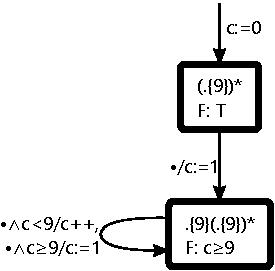
\includegraphics[width=3.6cm,keepaspectratio]{figures/dot9star_TB.pdf}
  \vspace*{-6mm}
\end{minipage}
  \caption{\label{fig:dot9star}$\CA(\regex{(\DOT\leftbrace9\rightbrace)*})$}%, with notation as in \cref{fig:ak:nondet}.}
\end{wrapfigure}
%
%%%%%%%%%%%%%%%%%%%%%%%%%%%%%%%%%%%%%%%%%
% UGLY HACK!
%%%%%%%%%%%%%%%%%%%%%%%%%%%%%%%%%%%%%%%%%
\paragraph{\it Example \arabic{section}.\arabic{theorem}.\,}
\stepcounter{theorem}
%%%%%%%%%%%%%%%%%%%%%%%%%%%%%%%%%%%%%%%%%
\!Consider the regex
\texttt{(\DOT\leftbrace9\rightbrace)*},
whose CA is in
\cref{fig:dot9star}. 
Here,  {\DOT} is the only input
predicate and denotes the set of all characters.
%
We explain the use of some of the counter operations in the CA of
\cref{fig:dot9star} 
by showing how they arise through the
partial-derivative-based construction of {\CA}s as discussed above. 
%
The initial
state is the regex itself. The (only) partial derivative of the state
\texttt{(\DOT\leftbrace9\rightbrace)*} is
\texttt{\DOT\leftbrace9\rightbrace(\DOT\leftbrace9\rightbrace)*} where the body
of the counting loop is exited but also incremented once, so $\ExitIncrOp$ is
applied to $c$ under the guard $\CanExit{c}$ (which is shown as $c\geq
9/ c{:=}1$ in the figure). 
 The state
\texttt{\DOT\leftbrace9\rightbrace(\DOT\leftbrace9\rightbrace)*} has \mbox{two cases
of partial derivatives both leading back to
\texttt{\DOT\leftbrace9\rightbrace(\DOT\leftbrace9\rightbrace)*}. }



The first
case is when $c < 9$ ($\CanIncr{c}$ holds), in which case $c$ is
incremented (shown as \ $c< 9/ c\mathtt{++}$ in the figure). The
second case is when the counting loop is conditionally nullable and is exited
under the condition  $\CanExit{c}$ (i.e. $c\geq 9$), the value of $c$ is
reset to 0, and then $c$ is incremented as a result of taking the partial
derivative of \texttt{(\DOT\leftbrace9\rightbrace)*}.  Thus, $\ExitIncrOp$
arises as a sequential composition of exiting the loop, followed by resetting
the counter to $0$, and then incrementing it. Therefore, $\CanExit{c}$ must
hold, while the increment condition holds trivially after a reset to $0$.  The
initial state is unconditionally final in 
%Figure~\ref{fig:9k}(a), 
\cref{fig:dot9star}, 
while the
other state is final only when $\CanExit{c}$ holds as marked by ``$F:$''.
\qed
\medskip

We now state the correctness theorem of conditional derivatives.
%
For that, we define $\CanExit{R}$ as the predicate shown above for a
normalized regex $R$, assuming that $X$ stands for a counting loop.
\[
\CanExit{R}\eqdef
\left\{
\begin{array}{ll}
  \top_{\CC} & \textrm{if $R=\emp$,}\\
  \CanExit{Z} & \textrm{else if $R=YZ$ and $Y$ is nullable,}\\
    \CanExit{X}\wedge\CanExit{Z} &\textrm{else if $R=XZ$,}\\
  \bot_{\CC} & \textrm{otherwise.}
\end{array}
\right.
\]
%
Note that $Y$ above may also be a counting loop.
%
However, since it is nullable, $\MIN{Y}$ must be $0$, and then $\CanExit{Y}$ is
always true.
%
(If $\MIN{Y}>0$, then $Y$ cannot be nullable as $R$ is normalized.)

We further need the following additional notions too.
%
A counter $X$ \emph{is visible in} $R$ if either $R=YZ$ and $X=Y$, or else if
$X$ does not occur in $Y$ and $X$ is visible in $Z$.
%
A counter memory $\mem$ is \emph{valid for} $R$ if $\mem(X)=0$ for all invisible
counters $X$ that occur in $R$.
%
Correctness of the construction of conditional derivatives is stated in
Theorem~\ref{theorem:CD}---see
\ifTR
Appendix~\ref{app:thmCD}
\else
\cite{OOPSLA20TR}
\fi
for a detailed proof. 


\begin{theorem}
  \label{theorem:CD}
Let $R$ be a normalized regex and let $\Sigma = \Minterms{\Theta}$
where $\Theta$ is some finite superset of $\REpreds{R}$. 
  If $\mem$ is valid for $R$, then
  $\LANG{\mem}{R} = \bigcup_{\alpha\in\Sigma}\den{\alpha}\cdot
  \LANG{\mem}{\CD{\alpha}{R}}\cup\{\eps\mid \mem\models\CanExit{R}\}$.
\end{theorem}

%==============================================================================
\subsection{Constructing CAs from Conditional Derivatives}\label{sec:ca-construction}
%==============================================================================

We convert a normalized regex $R$ to the counting automaton $\CA(R)$ whose set
of states is the smallest set containing $R$ as the initial state and all those
regexes that arise in conditional derivatives constructed from $R$ by repeated
derivation wrt $\Sigma$.
%
Given a state represented by a regex $S$, for each $\alpha\in\Sigma$ and each
partial conditional derivative $\pair{f}{T} \in \CD{\alpha}{S}$, there is a
transition $\move{S}{\alpha,f}{T}$ in $\CA(R)$.
%
The \emph{final condition} $F(S)$ of a state $S$ of $\CA(R)$ is $\CanExit{S}$.
Observe that $F(S)=\bot_\CC$ when $S$ is not nullable and has no visible
counters, which corresponds to the classical case.

As shown in
\ifTR
Appendix~\ref{appThmDeriv}
\else
\cite{OOPSLA20TR}
\fi
the following result can be proved using
Theorem~\ref{theorem:CD}.

\begin{theorem}
\label{thm:deriv}
Let $R$ be a normalized regex and $A=\NFAof{\CA(R)}$.
Then, for all $\pair{\mem}{S}\in Q_A$,
$\Lq[A]{\pair{\mem}{S}} = \LANG{\mem}{S}$.
\end{theorem}

The construction of $\CA(R)$ terminates, and the number of states of $\CA(R)$ is
linear in $\LEAFCNT{R}$.

\begin{theorem}
  \label{theorem:SIZE}
  Let $R$ be a normalized regex. Then $|Q_{\CA(R)}|\leq\LEAFCNT{R}+1$.
\end{theorem}

A proof of Theorem~\ref{theorem:SIZE} is in
\ifTR
Appendix~\ref{app:theorem:SIZE}.
\else
\cite{OOPSLA20TR}.
\fi
We get the following final correctness result as a corollary of
Theorem~\ref{thm:deriv}, Theorem~\ref{thm:LANG}, and Theorem~\ref{theorem:SIZE}.

\begin{corollary}
  \label{cor:deriv}
Let $R$ be a normalized regex. Then $\langof{R}  = \langof{\CA(R)}$.
\end{corollary}

\begin{proof}
  First, $Q_{\CA(R)}$ is finite, and thus well-defined by using Theorem~\ref{theorem:SIZE}.
  Use Theorem~\ref{thm:deriv} with 
  $\pair{\mem}{S}$ as the initial state $\pair{\memInit}{R}$ of $A$.
  It follows that $\langof{A} = \LANG{\memInit}{R}$.
  Then use Theorem~\ref{thm:LANG} for $\LANG{\memInit}{R}=\langof{R}$
and $\langof{\CA(R)}=\langof{A}$ holds by definition.
\end{proof}

A further important aspect of $\CA(R)$ is that,
although the number of input minterms may potentially be exponential
in the number of predicates in $R$, in the case of predicates being
represented as a finite union of intervals (as is done typically for
character classes), the size of a single predicate representation can
be estimated to be proportional to the number of interval borders in
the union.  In this case, the total size of all the minterms remains
linear in the total size of all the predicates because the total
number of interval borders will remain the same in minterms as in the
original set of predicates.  In other words, mintermization based on
character classes does not blow up the number of transition in
$\CA(R)$. We have also validated this fact experimentally.

%%%%%%%%%%%%%%%%%%%%%%%%%%%%%%%%%%%%%%%%%%%%%%%%%%%%%%%%%%%%%%%%%%%%%%%%%%%%%%%%
\section{From Counting Automata to Counting-Set Automata} \label{sec:algo-idea}
%%%%%%%%%%%%%%%%%%%%%%%%%%%%%%%%%%%%%%%%%%%%%%%%%%%%%%%%%%%%%%%%%%%%%%%%%%%%%%%%

{\CA}s obtained through conditional derivatives as shown in the previous section
are nondeterministic.
%
As one of the main contributions of this work, we now propose an approach for
determinizing them into a form that can be used efficiently for regex matching. 
%
The approach from which we start and to which we contrast our new method is the
naive determinization of {\CA}s to DFAs:
%
The given CA is first converted to its underlying NFA, by making the counter
memories an explicit part of control states.
%
The NFA is in turn determinized by the textbook subset construction. 

Already the first step, the construction of the NFA, oftentimes explodes since
it sacrifices the succinctness of symbolic counters (it is linear to the counter
bounds).
%
This initial blow-up is then much amplified in the subset construction, which is
exponential to the size of the NFA and hence also to the counter bounds (as,
e.g., in the case of the regex \regex{\DOT*a\DOT\{$k$\}} with its CA
in~\cref{fig:ak:nondet}).

Our answer to this problem is a direct determinization of the CA into a novel type
of automata, which we call \emph{counting-set automata ({\CSA}s)}.
%
Control states of counting-set automata produced by our determinization are
essentially the states of the corresponding DFA but with the counter memories
removed.
%
In order to be able to simulate a run of the DFA, they  are equipped with
special registers that can hold \emph{sets} of integers, and they use them to
compute the right counter memories at runtime.
%
This completely avoids the state space explosion of the naive construction
caused by wiring counter memories into control states.
%
Moreover, the simulation is fast because all the manipulations with a
counting set can be done in constant time. 

%==============================================================================
\subsection{Counting-Set Automata}
%==============================================================================
\label{sec:CsA}

We now formalize the idea of counting-set automata outlined above.  We
use the notion of a~combined Boolean algebra $\IICCS$, which allows us to
manipulate pairs of predicates from the input algebra $\II$ and the
counting-set algebra $\CCS$. For the purposes of this paper, we assume
that predicates in $\PRED_{\IICCS}$ have the form $\alpha\wedge\beta$
where $\alpha\in\PRED_{\II}$ and $\beta\in\PRED_{\CCS}$. The conjuction
$(\alpha\wedge\beta)\wedge_{\IICCS}(\alpha'\wedge\beta')$ has the usual meaning
of $(\alpha\wedge_{\II}\alpha')\wedge(\beta\wedge_{\CCS}\beta')$ and
$\alpha\wedge\beta$ \mbox{is satisfiable if both $\alpha$ and $\beta$ are
satisfiable in their respective algebras.}

%------------------------------------------------------------------------------
\paragraph{Counting sets.}
%------------------------------------------------------------------------------

We consider a set-based interpretation of counters where the value of a counter
$c$ is a \emph{finite set} rather than a single value. 
%
A counter under such an interpretation is referred to as a \emph{counting set}.
%
A \emph{(counting-)set memory} for $C$ is a function $\smem : C \rightarrow
\PowerSetNE{\nat}$ such that, for all $c\in C$, $\MaxOf{\smem(c)} \leq
\MAX{c}$.\footnote{We write $\PowerSetNE{X}$ for the powerset of $X$ restricted
to finite nonempty sets.}
%
Observe that the set of all set memories for $C$ is \emph{finite}.
%
Counting-set predicates over $C$ form an effective Boolean algebra $\CCS_C$ called
the \emph{counting-set algebra over $C$}, 
also denoted just $\CCS$ when $C$ is clear from the context, 
whose domain $\DOM_{\CCS}$ is the set
of all set memories for $C$.
%
The set of predicates $\PRED_{\CCS}$ is the Boolean closure of the basic
predicates $\CanIncrS{c}$ and $\CanExitS{c}$, hence syntactically the same as in
the counter algebra $\CC$, but with a different semantics under $\CCS$:
%
$$\smem\models \CanExitS{c} \Iff \MaxOf{\smem(c)} \geq \MIN{c}
\quad\textrm{and}\quad \smem\models\CanIncrS{c}\Iff \MinOf{\smem(c)} < \MAX{c}$$
where $\MinOf\cdot$ and $\MaxOf{\cdot}$ are the set minimum and maximum,
respectively. 
%
Intuitively, the conditions test existence of a set element satisfying the same counter condition.

%------------------------------------------------------------------------------
\paragraph{Counting-set automata.}
%------------------------------------------------------------------------------
A \emph{counting-set automaton} (\CSA) is a tuple $A =
(\II,C,Q,q_0,\FinCond{},\Delta)$ where:
%
$\II$~is an effective Boolean algebra called the \emph{input algebra}.
%
$C$ is a finite set of \emph{counters} associated with the counting-set algebra
$\CCS$.
%
$Q$ is a finite set of \emph{states} with $q_0\in Q$ being the \emph{initial
state}.
%
$\FinCond{}: Q\rightarrow\PRED_{\CCS}$ is the \emph{final-state condition}.
%
$\Delta \subseteq Q\times\PRED_{\IICCS}\times(C \rightarrow \PowerSet{\OPS})\times Q$ is a finite set of \emph{transitions}.
% 
The second component is its \emph{guard}.
The third component is the
\emph{counting-set operator} in which $\OPS = \{\IncrCSOp, \NoCSOp, \ExitCSOp,
\ExitIncrCSOp\}$ is the set of \emph{counting-set operations}.
%
They are essentially counter operations lifted to sets 
(note the use of the larger initial letters to distinguish them from the counter operations).
We also use the different names 
 $\ExitCSOp$ and
$\ExitIncrCSOp$ for the lifting of
$\ExitOp$ and $\ExitIncrOp$ 
to stress their different usage
(not only for exiting a loop but also for initialisation when entering the
loop as will become clear in \cref{eq:caoptocsa}). 
\cbstart
Sets of counting-set operations assigned to every counter by the counting-set operator are called \emph{combined (counting-set) operations}.
\cbend

The {\CSA} $A$ is \emph{deterministic} iff the following holds for every two transitions 
$\move p {\psi_1, f_1} {q_1}$ and  $\move p {\psi_2, f_2} {q_2}$ in $\Delta$: 
if $\psi_1 \wedge \psi_2$ 
is satisfiable, then $f_1 = f_2$ and $q_1 = q_2$.

%------------------------------------------------------------------------------
\paragraph{Semantics of {\CSA}s.}
%------------------------------------------------------------------------------

The semantics of an indexed counting-set operation $\Op[c] \in \OPS$ is the set
transformer $\update{\Op[c]}$ defined as follows:   
%
$$
\begin{array}{r@{\ =\ }lr@{\ =\ }l}
\update{\IncrCSOp[c]} & \blambda S.\{n+1\mid n\in S \land n < \MAX{c}\} & \update{\ExitCSOp[c]} & \blambda S.\{0\}\\
\update{\NoCSOp[c]} &\blambda S.S & \update{\ExitIncrCSOp[c]} & \blambda S.\{1\}
\end{array}
$$
%
Then, the counting-set operator $f:C\rightarrow\PowerSet{\OPS}$ is assigned the
counting-set-memory transformer $\Update{f}:\DOM_{\CCS}\rightarrow\DOM_{\CCS}$
defined as follows: 
%
 $$ \Update{f}(\smem) \eqdef \blambda c.\left\{ \begin{array}{ll} \bigcup_{\Op\in f(c)}
 \update{\Op[c]}(\smem(c)) & \text{if}\ f(c)\neq \emptyset \\ \{0\} &
 \text{if}\ f(c)=  \emptyset \end{array} \right.  $$
%
That is, (1) if $f(c)\neq \emptyset$, then the value $\smem(c)$ of each counting
set $c$ is transformed into the union of the counting sets that result from
applying the operations from $f(c)$ on $\smem(c)$, and
%
(2) if $f(c) = \emptyset$, then $c$ is implicitly reset to $\{0\}$ (an implicit $\ExitCSOp$). 
Our determinization procedure creates such transitions when the value of $c$ is irrelevant 
(when $c$ is a dead variable). 

Note that, unlike counter operators of a CA, a counting-set operator $f$ does
not induce any guard.
%
The guard is rather a separate component of the transition.
%
This is because CsA transitions produced in the CA-to-CsA determinization need
guards that are partially independent of the operations of $f$.
%
In particular, we will we need to distinguish cases such as
$\neg\CanExit{c}\wedge\CanIncr{c}$, $\CanExit{c}\wedge\neg\CanIncr{c}$, or
$\CanExit{c}\wedge\CanIncr{c}$.
%
The guard hence cannot be induced by $f$ alone. 

Note also that, unlike in CAs, the updates are defined for \emph{indexed}
operations.
%
The reason is that the semantics of the $\IncrCSOp$ operation is restricted to
never produce values greater than $\MAX{c}$.

Finally, the \emph{language of the CsA} $A$ is defined through its 
%
underlying  \emph{configuration FA}, $\NFAof{A}$, as $\langof{A} :=
\langof{\NFAof{A}}$.
%
The states of $\NFAof{A}$ are \emph{configurations} of $A$, namely, tuples of
the form $(q,\smem) \in Q \times \DOM_{\CCS}$ consisting of a state $q$ and a
counting-set memory~$\smem$.
%
There are finitely many such configurations.
%
The initial state of $\NFAof{A}$ is the \emph{initial configuration}
$(q_0,\{c\mapsto\{0\}\}_{c\in C})$~of~$A$.
%
A~transition $\tau=\move p {\alpha\land\beta, f} q\in \Delta$ is \emph{enabled} in a
configuration $(p,\smem)$ iff $\alpha$ is satisfiable and
$\smem\in\den[\CCS]{\beta}$, meaning that $\smem$ satisfies the counter guard $\beta$.
If $\tau$ is enabled in $(p,\smem)$, then $\NFAof{A}$ contains the transition
$\move{(p,\smem)} {\alpha} {(q,\Update{f}(\smem))}$. 
%\cbend
Finally, a state $(q,\smem)$ of $\NFAof{A}$ is \emph{final} iff
$\smem\models\FinCond{q}$.

\begin{ex} An example of a CsA is in \cref{fig:ak:det}. It uses intuitive
  notations that were also introduced in \cref{sec:overview} as
  abbreviations for the operations of the counting-set data structure.
Counting-set operators are
depicted as assignments to $c$, $\ExitCSOp$ is represented as $\{0\}$ on the
right of the assignment, $\ExitIncrCSOp$ is represented by $\{1\}$, $\IncrCSOp$
by $c+1$, and $\NoCSOp$ by~$c$. Multiple transitions between the same states and
with the same updates are merged into one with a simplified guard. An example
whose notation closely follows the formal development is in
  \cref{fig:detsample}.
\end{ex}

%------------------------------------------------------------------------------
\paragraph{Runtime efficiency of counting sets.}
%------------------------------------------------------------------------------

\cbstart
A major reason for choosing CsAs as the target kind of machine for
determinization of CAs is that pattern matching with CsAs is fast.
%
% As explained in \cref{sec:overview},   
%
Using the data structure explained in \cref{sec:overview}, all the basic
counting-set tests and updates, namely,  $\CanIncr c$, $\CanExit c$, $\NoCSOp$,
$\IncrCSOp$, $\ExitCSOp$, and $\ExitIncrCSOp$, can be implemented to run in
constant time regardless of the size of the counting set and the value $\MAX{c}$
(assuming constant-time complexity of integer arithmetic operations).
%
Moreover, almost all combined counting-set operations can be implemented to run
in constant time too. 
%
In particular, when at most one counting-set operation of a given combined
operation returns a set other than $\{0\}$ or $\{1\}$, their union can be
computed in constant time.
%
% The only difficulty arises when the combined operation has two member
% counting-set operations that may return non-singleton sets. 
%
% Their union is then liner to the size of these sets (which is at most $\MAX
% c$).
%
If this is not the case, the union is linear to the size of the sets computed by
the particular counting-set operations (which is at most $\MAX c$).
%
The only operations that may return sets other than $\{0\}$ or $\{1\}$ are
$\NoCSOp$ and $\IncrCSOp$. 
%
We denote a transition whose counting-set operator $f$ assigns to some counter
$c$ the result of a combined operation $f(c)$ that contains both $\NoCSOp$ and
$\IncrCSOp$ as \emph{slow}.
%
A CsA that has slow transitions is called \emph{slow}, and a CsA that does not
have them is called \emph{fast}.
%
Slow CsAs are fortunately rare in practice (cf. \cref{sec:experiments}). 
 
When a fast CsA is used in pattern matching, tests and updates of one counting
set then take $\bigo(1)$ time, which in turn gives $\bigo(|C|)$ for all counting
sets and their unions.
%
\emph{This is our major achievement: the independence of the running time from
the counter bounds.}
\cbend

%==============================================================================
\subsection{Encoding DFA Powerstates as CsA Configurations}\label{sec:nonzero}
%==============================================================================

In order to build intuition needed for understanding our determinization
algorithm, we will first concretize how the configurations of a CsA can encode
states of a DFA corresponding to the NFA $\NFAof{A}$ underlying a given CA
$A=(\II,C,Q,q_0,F,\Delta)$.
%
First, recall that, since $A$ is converted into $\NFAof{A}$ by making the
counter memories explicit parts of control states, the states of $\NFAof{A}$ are
pairs $(p,\mem)$ consisting of a~state $p$ of~$A$ and a counter memory $\mem$. 
%
Second, assume that $\NFAof{A}$ is determinized using the textbook subset
construction.%
%
\footnote{The DFA produced by the textbook subset construction from a
\emph{simple} FA $\mathcal{A} = (\II,Q,q_0,F,\Delta)$ will have  $\PowerSet{Q}$
as the set of states, transitions $\move{S}{\alpha}{\{r\in Q\mid
\move{s}{\alpha}{r}\in\Delta,s\in S\}}$, the initial state $\{q_0\}$, and as the
final states all those intersecting $F$.
%
We note that to determinize a CA which is not simple, one could start from the
more sophisticated version of the subset construction for symbolic automata of
\cite{SFAdeterm}, which avoids explicit generation of all minterms.}
%
We denote the result as $\DFAof{A}$ from now on.
%
Then, the states of~$\DFAof A$ are sets of states of~$\NFAof{A}$, i.e., sets of
pairs $(p,\mem)$, which we will call \emph{powerstates}.
%
The control states of the CsA $\CS{A}$ built by our CA-to-CsA determinization
will be subsets of the set $Q$ of states of the CA $A$.
%
The configurations of $\CS{A}$ will thus be pairs $(R,\smem)$ where $R\subseteq
Q$ is a CsA control state, i.e., a set of states of $A$, and $\smem: C
\rightarrow \PowerSetNE{\nat}$ is a counting-set memory. 
%
Let us now consider how $\smem$ can be interpreted in this context.

%------------------------------------------------------------------------------
\paragraph{Naive encoding.}
%------------------------------------------------------------------------------

A naive interpretation of a CsA configuration $(R,\smem)$ is
a DFA state containing all pairs $(r,\mem)$ such that
$r\in R$ and, for all $c\in C$, $\mem(c)$ can be any value from $\smem(c)$.
%
The set of the counter memories $\mem$ is then isomorphic to 
the Cartesian product $\prod_{c\in C}\smem(c)$ of the sets  $\smem(c)$ assigned to the counters, 
and the entire powerstate is the Cartesian product $R\times \mem$ of the set of states and the set of counter memories.
%
The naive interpretation, however, is too impractical as it cannot express any
dependence of a counter memory on the CA state (every state can be paired with
each considered memory) nor any mutual dependence of values of different
counters within a counter memory (every possible value of a counter $c$ can be
paired with every possible value of any other counter $d$).
%
Most DFAs compiled from real-life regexes do not fit into this
representation.
%
For instance, the DFA configuration $\{(q,c=0),(s,c=0),(s,c=1)\}$ of the CA from
\cref{fig:ak} in \cref{sec:overview} could not be represented by a CsA
configuration because $q$ and $s$ appear with different sets of counter values.

%------------------------------------------------------------------------------
\paragraph{Encoding with counter scopes.}
%------------------------------------------------------------------------------

Our key observation how to resolve the above problem (at least for many
real-life scenarios) is to take advantage of that not every counter is ``used''
at every CA state. 
%
In fact, the value of a counter is usually implicitly 0 at most states except a
few. 
%
If these states are known, the implicit zeros do not have to be remembered
explicitly in the counting sets, and the encoding becomes much more flexible. 
%
To formalize this, we introduce the notion of the \emph{scope of a counter} that
over-approximates the set of states where a counter $c$ can have a non-zero
value and that is easy to compute.\footnote{Computing the precise set of states
where a counter $c$ can have a non-zero value would require a reachability
analysis in the general case (since some of the transitions may never be
executable---think of simultaneously counting with counters $c$ and $d$ such
that $\CanIncr c < \CanExit d$, then the exit transition for $d$ will never be
taken). For the CAs made by our derivative construction, the scope, however,
corresponds to this set \mbox{precisely---no transitions that are never
executable are generated.}
}
%
The scope is defined inductively as the smallest set of states $\scope(c)$ such
that\begin{enumerate}

  \item $q \in \scope(c)$ if there is a transition to $q$ with either $\IncrOp[c]$
  or $\ExitIncrOp[c]$, or

  \item there is a transition to $q$ from a state in $\scope(c)$ with the
  $\NoOp[c]$ operation.

\end{enumerate} In other words, the scope of $c$ spreads from an increment of
$c$ along the transition relation until a transition with $\ExitOp[c]$.

The DFA \emph{powerstate encoded by a CsA configuration} $(R,\smem)$ can then be
formally defined as the set $\pstateof{(R,\smem)}$ of configurations $(r,\mem)$
of the CA $A$ such that $r\in R$ and, for all $c\in C$, $\mem(c)\in \smem(c)$ if
$c\in\scope(r)$, else $\mem(c) = 0$.
%
We call the powerstates of $\DFAof{A}$ that can be encoded by CsA configurations
\emph{Cartesian}, and call the entire DFA Cartesian if all its
powerstates are Cartesian.

\begin{ex}
The powerstates of the $\DFAof{A}$ of the \CA $A$ from \cref{fig:ak:nondet} are
indeed Cartesian (as discussed in \cref{sec:overview}) because $q_0$ is not in
the scope of $c$.
The encoding of powerstates by CsA configurations is also illustrated in \cref{sec:overview} and later also in \cref{ex:det_trans_constr}.
\end{ex}


The Cartesian encoding still cannot express all kinds of DFA powerstates.
%
In particular, it cannot express more subtle dependencies of counter values on the state, and dependencies of counter values of different
counters on each other, which mainly concerns CAs with nested counting loops
compiled from regexes with nested counting sub-expressions. 
%
\cref{ex:noncartesian} discusses a regex that leads to a non-Cartesian CA. 
%
However, we later present a strong empirical evidence that a significant
majority of real-life regexes lead to Cartesian CA. 

%==============================================================================
\subsection{Generalized Subset Construction}\label{sec:subscons}
%==============================================================================

We will now describe the core of our CA-to-CsA determinization.
%
It is built on top of the textbook subset construction for NFAs.
%
We use the CA from \cref{fig:detsample:CA} as a running example through the
section.
%
We make a simplifying assumption that the input CAs are simple (different
character classes on their transitions do not overlap). This is satisfied by CAs
generated by the derivative construction from \cref{sec:regexes} since their transitions are labeled by minterms of the original regex. 
%
The assumption could be dropped and the construction could be relatively easily generalized in the style of symbolic automata determinization of \cite{SFAdeterm}.


Let $A=(\II,C,Q,q_0,F,\Delta)$ be a simple 
CA with the scope function
$\scope:Q\rightarrow\PowerSet{C}$. 
%
The algorithm produces the deterministic CsA
$\CS{A}=(\II,C,\CS{Q},S_0,\CS{F},\CS{\Delta})$ whose components are constructed
as described below.
%
Namely, control states of $\CS{A}$, called powerstates, are subsets of $Q$,
i.e., $Q' \subseteq \PowerSet Q$.
%
The initial powerstate is $S_0 = \{q_0\}$.
%
A powerstate $S\in \CS{Q}$ is final iff the final condition holds for some of
its elements, i.e., $\CS{F}(S)\eqdef\bigvee_{q\in S} F(q)$.
%
The sets $\CS{\Delta}$ and $\CS{Q}$ are constructed by a fixpoint computation
that explores the state space reachable from $S_0$.
%
During the construction, transitions starting from previously reached
powerstates are constructed and included together with their target states into
$\CS{\Delta}$ and $\CS{Q}$, respectively, until no new powerstates can be
reached.  

Transitions starting from a given control state $R$ of the CsA $\CS{A}$ are
constructed
%
to update the runtime values of counting sets such that they simulate
transitions of the DFA corresponding to the CA $A$.  
%
Assume a CsA configuration $(R,\smem)$ and a DFA transition
$\move{\pstateof{(R,\smem)}}{\alpha}{P}$ from the DFA powerstate encoded by
$(R,\smem)$ over an input minterm $\alpha$.
%
The simulating CsA transition must transform $(R,\smem)$ into $(R',\smem')$ with
$\pstateof{(R',\smem')} = P$.
%
The simulated DFA transition was constructed from $\alpha$-transitions of the
NFA $\NFAof{A}$ that are actually instantiations of the CA $\alpha$-transitions
enabled in configurations $(r,\mem)\in \pstateof{(R,\smem)}$. 
%
The simulating CsA transition will be constructed from these CA transitions. 
%
They can be identified by (1)~their source state, which must be in $R$, (2)~an
alphabet minterm $\alpha\in\Sigma$ where $\Sigma$ is the set of minterms over
all input predicates in the CA $A$, 
and (3)~their compatibility with a particular set
of enabled/disabled counter guards.
%
This set of guards belongs to the set of minterms $\Gamma_{R,\alpha}$ of the set
of counter guards on the $\alpha$-transitions originating in $R$:
$$\Gamma_{R,\alpha} \defeq \Minterms{\{\guard{\Op[c]}\mid
\move{r}{\alpha,f}{s}\in \Delta, r\in R \land c \in \scope(r), \Op[c]\in f\}}.$$
%
Hence, the CsA will have a transition leaving $R$ for each $\alpha\in \Sigma$
and
$\beta\in\Gamma_{R,\alpha}$, and the transition will be built from the set of CA
$\alpha$-transitions originating in $R$ and \emph{consistent} with $\beta$: 
%
\begin{equation*} \label{eq:consistent} 
\consistent \eqdef \{
\move{r}{\alpha,f}{s}\in\Delta\mid r{\in} R, \SAT(\Guard{f}\land \beta) \}.
\end{equation*}
%
Its target is the set $T$ of all target states of the transitions in
$\consistent$, and its guard is $\alpha \land \beta$.\footnote{Recall that
the predicates in $\PRED_\CC$ and $\PRED_\CCS$ are syntactically the same.}


The remaining component is the counting-set operator $\CS{f}$.
%
It must summarize the updates of the counter values on transitions of
$\consistent$ as updates of the respective counting sets. 
%
The values of counters that are out of scope, hence implicitly zero, will not be
tracked in counting sets.
%
Tracking the value of a counter hence starts when $\CS{A}$ simulates a
transition of $A$ entering the scope of the counter, and ends when no state from
the scope is present in the target CsA state. 

\begin{wrapfigure}[8]{r}{63mm}
\begin{minipage}{65mm}
  \vspace*{-5.5mm}
  \begin{equation*}
  \textit{op}(\,\move {p\!}{\alpha,f}{\!q}\,,c) \defeq \hfill
  \end{equation*}
  \vspace*{-2mm}
  \hspace*{-6mm}
  \begin{minipage}{67mm}
      \begin{equation}
  \label{eq:caoptocsa}
      \defeq
      \left\{ 
      \begin{array}{ll}
        \NoCSOp 		& \text{if $f(c) = \NoOp \wedge p\in\scope(c)$}\\
        \IncrCSOp 		& \text{if $f(c) = \IncrOp \wedge p\in\scope(c)$}\\
        \ExitCSOp		& \text{if $f(c) = \NoOp \wedge p\not\in \scope (c)$}\\  
        \ExitIncrCSOp	& \text{if $f(c) = \IncrOp \wedge p\not\in\scope(c)$}\\
        \ExitCSOp 		& \text{if $f(c) = \ExitOp$}\\
        \ExitIncrCSOp	& \text{if $f(c) = \ExitIncrOp$}\\
    \end{array}
    \right.
    \end{equation}
  \end{minipage}
\end{minipage}
\end{wrapfigure}

Let $\consistent(c)$ be the set of transitions in $\consistent$ with the target
state in the scope of $c$.
%
The counting-set operator $\CS{f}$ is built in the form
$\CS{f}(c)\eqdef\{\textit{op}(\tau,c)\mid \tau\in \consistent(c)\}$.
%
Here, $\textit{op}(\tau,c)$ denotes the counting-set operation that, given a CA
transition $\tau = \move p {\alpha,f} q$, transforms the set of possible values
of the counter $c$ at the state $p$ to the set of values obtained at $q$ after
taking the transition.
%
It is defined in \cref{eq:caoptocsa} on the right.
%
The set operation induced by the CA transition corresponds to the counter
operation on the transition. 
%
In the third and fourth case, when the CA transition comes from out of the
scope, it is certain that the counter can only have the value $0$, which is the
same value as produced by $\ExitOp$ (or $\ExitIncrOp$ when the counter is
immediately incremented).
%
The resulting CsA transition is therefore $\move S {\alpha\land\beta,\CS{f}} T$.
%
Note that $\CS{f}(c)$ ends up empty when the target powerstate is fully out of
the scope of $c$, which semantically corresponds to the implicit reset to $\{0\}$.

Observe that $\CS{A}$ is deterministic
since, for any two distinct transitions
$\move{S}{\alpha_1,f_1}{S_1}$ and
$\move{S}{\alpha_2,f_2}{S_2}$, the condition
$\alpha_1\wedge\alpha_2$ is unsatisfiable
by virtue of minterms. 

\begin{figure}
  %\ \\[-10mm]
  \vspace{-3mm}
  \hspace{-10mm}
  \begin{subfigure}[b]{0.24\linewidth}
  \begin{center}
    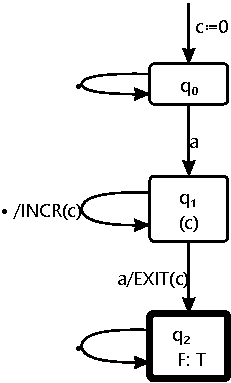
\includegraphics[height=4.6cm,keepaspectratio]{figures/detsample_TB.pdf}
  \end{center}
%  \caption{The CA for \texttt{\DOT*a\DOT{\leftbrace}4,8{\rightbrace}a}}
  \label{fig:detsample:CA}
  \end{subfigure}
  \hspace{2mm}
  \begin{subfigure}[b]{0.64\linewidth}
  \begin{center}
    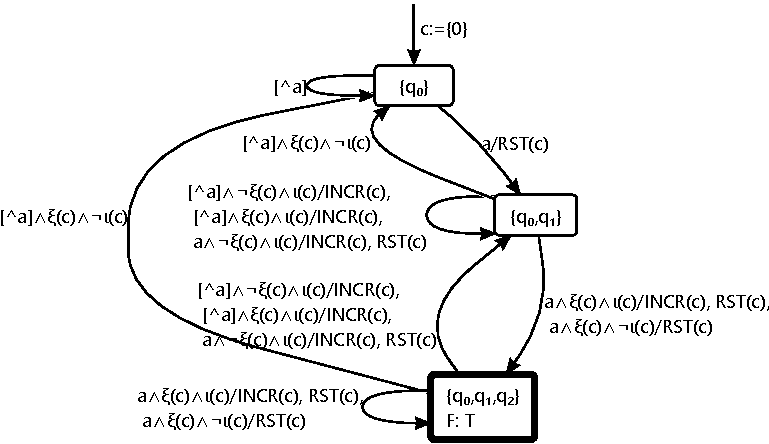
\includegraphics[height=5.6cm,keepaspectratio]{figures/detsampleCSA_TB.pdf}
    %\vspace*{-8mm}
  \end{center}
  \caption{Determinization of the CA into a {\CSA}}
  \label{fig:detsample:CsA}
  \end{subfigure}
  \caption{From a regex via a CA to a deterministic CsA. 
    We are using a notation closely following the formal development. 
    We only use $\Op(c)$ instead of $\Op[c]$ and abbreviate  
    $\CanExitS c$ by $\xi(c)$ and $\CanIncrS c$ by $\iota(c)$.
  }
  \label{fig:detsample}
  \vspace{-2mm}
\end{figure}
%

\begin{theorem}
  For the CA $A$ and the CsA $\CS A$ above, we have $\langof {\CS \aut} \supseteq \langof \aut$ and $|\CS
  Q| \leq 2^{|Q|}$.
\end{theorem}
\begin{proof}[Proof (idea)] 
The language inclusion is proved by showing that the configuration automaton $\FA(\CS A)$ of $\CS A$ simulates $\DFAof A$,
more concretely, that each configuration $(R,\smem)$ of $\CS A$, a state of $\FA(\CS A)$,
simulates the powerstate $(R,\smem)$ of $\DFAof A$.
%
The bound on the size of the state space follows from that states of the CsA are
sets of states of the CA.\end{proof}

\begin{ex}\label{ex:det_trans_constr} Consider the {\CA} in
\cref{fig:detsample:CA} that has states $q_0$, $q_1$, and $q_2$.
%
The state $q_0$ is initial, the final condition of $q_2$ is $\top$, and it is
$\bot$ for $q_0$ and $q_1$.
%
The set of counters is $C= \{c\}$ with $\scope(c) = \{q_1\}$ (i.e., $c$ is not
used and hence implicitly 0 in $q_0$ and $q_2$).
%
Finally, $\Sigma = \{\regex{a},\notacl\}$.
%
In \cref{fig:detsample:CA}, we compactly represent transitions over all minterms
from~$\Sigma$ using $\DOT$.
%
The determinization starts exploring the CsA from its initial state $S_0 =
\{q_0\}$. 

Let us focus on the transitions for the input minterm $\alpha = \acl$.
%
Two transitions leaving~$q_0$, namely $\delta_1 =
\move{q_0}{\acl,\NoOp[c]}{q_0}$ and $\delta_2 = \move{q_0}{\acl,\NoOp[c]}{q_1}$,
both with no guard on~$c$,
hence $\Gamma_{S_0,\alpha} = \{\top\}$. 
%
The guard~$\top$ is thus the only choice for the counter minterm $\beta$.
%
The set $\consistent$ of transitions consistent with $\alpha$ and $\beta$ then
contains both $\acl$-transitions $\delta_1$ and $\delta_2$ originating from $q_0$.
%
Since $\delta_2$ is entering the scope of $c$, it generates the counting-set
operation $\ExitCSOp[c]$ according to the third case of \cref{eq:caoptocsa}.
%
Since $\delta_1$ stays out of the scope, it does not generate any counting-set
operations.
%
We obtain the counting-set operator \mbox{$\CS{f} = \{\ExitCSOp[c]\}$ and generate the
CsA transition $\tau_1 =
\move{\{q_0\}}{\acl\land\beta,\{\ExitCSOp[c]\}}{\{q_0,q_1\}}$.}


Next, let us focus on the $\acl$-transitions from $S_1 = \{q_0,q_1\}$.
Here, $\Gamma_{S_1,\acl}$ has the following three satisfiable elements: $\CanExit{c}\land
\CanIncr{c}$,  $\neg\CanExit{c}\land \CanIncr{c}$, and  $\CanExit{c}\land
\neg\CanIncr{c}$ (the guard $\neg\CanExit{c}\land \neg\CanIncr{c}$ is excluded as it is
never satisfied for non-empty sets of positive integers).  
%
Let us generate a transition for the second case, $\beta = \neg\CanExit{c}\land
\CanIncr{c}$.
%
We obtain $\Delta_{S_1,\acl,\beta} =
\{\move{q_0}{\acl,\NoOp[c]}{q_0}$, $\move{q_0}{\acl,\NoOp[c]}{q_1}$, $\move{q_1}{\acl,\IncrOp[c]}{q_1}\}$. 
%
As before, the first transition does not contribute to $\CS{f}$ as it stays
out of the scope, and the second transition adds $\ExitCSOp[c]$.
%
The third transition adds $\IncrCSOp[c]$ (the second case of
\cref{eq:caoptocsa}).
%
The resulting CsA transition is thus $\tau_2 =
\move{S_1}{\acl\land\neg\CanExit{c}\land \CanIncr{c},\{\IncrCSOp[c],\ExitCSOp[c]\}}{S_1}$.
%
The rest of the construction is analogous.

Last, let us also illustrate the simulation of $\DFAof{A}$ by the constructed
CsA transitions.  
%
On the word $aa$, the DFA would execute the run
$\move{\move{\{(q_0,c=0)\}}{\acl}{\{(q_0,c=0),(q_1,c=0)\}}}{\acl}{\{(q_0,c=0),(q_1,c=0),(q_1,c=1)\}}$. 
%
The simulating run of our CsA would start in the initial configuration
$\{\{q_0\},c\in\{0\}\}$.  The transition $\tau_1$ would produce the
configuration $\{\{q_0,q_1\},c\in\{0\}\}$ (since $\ExitCSOp(\{0\}) = \{0\}$)
from where $\tau_2$ would produce $\{\{q_0,q_1\},c\in\{0,1\}\}$ (since
$\IncrCSOp(\{0\}) = \{1\}$ and $\ExitCSOp(\{0\}) = \{0\}$).
%
The sequence of configurations precisely encodes the sequence of the DFA
powerstates, that is, the sequnce
%
%Indeed, we obtain the sequence of DFA powerstates $\pstateof{(\{q_0\},c\in\{0\})}  = \{(q_0,c=0)\}$;
%Indeed, the sequence of DFA powerstates is $\pstateof{(\{q_0\},c\in\{0\})}  = \{(q_0,c=0)\}$;
$\pstateof{(\{q_0\},c\in\{0\})}  = \{(q_0,c=0)\}$;
$\pstateof{(\{q_0,q_1\},c\in\{0\})}  = \{(q_0,c=0),(q_1,c=0)\}$; and
$\pstateof{(\{q_0,q_1\},c\in\{0,1\})}  = \{(q_0,c=0),(q_1,c=0),(q_1,c=1)\}$
(recall that $q_0$ is not in the scope of $c$ hence $c$ has implicitly the
value 0 there).  
\end{ex}







 \begin{figure}[t]
%\vspace{-3mm}
\begin{center}
\begin{algorithm}[H]
\caption{DFA-based space search}
\label{algo:basic}
\KwIn{A DFA $\aut =(\II,Q,q_0,F,\Delta)$.}
\KwOut{an ouptut string $string$.} 
    $unvisited \leftarrow \{q_0\}$\;
    $visited \leftarrow \emptyset$\;
    $str \leftarrow \epsilon$\;
    $successors:=\{ (q_0\mapsto q_0)\}$\;
    \While{$unvisited \neq \emptyset$}{
    $q \leftarrow ChooseBest (unvisited)$\;
    $str\leftarrow str \cdot Prefix(q, successors)$\;
    
    \While{$not (timeout)$}{
    $T\leftarrow\{(q, \alpha, r)\in \Delta | r \not \in F\}$\;
    \lIf{$T == \emptyset$}{break}
    \Else{
 	   	$(q', \alpha', r') \leftarrow SelectBest(T)$\;
 	   	remove $(q', \alpha', r')$ from $T$\;
   	 	$unvisited\leftarrow unvisited \cup \{r | (q, \alpha, r) \in T\}$\;
    		$visited \leftarrow visited \cup \{r'\}$\;
   	 	$successors\leftarrow successors\cup \{(q\mapsto r')\}$\;
   		$q\leftarrow r'$\;
    		$str \leftarrow str \cdot ChooseSymbol(\alpha)$\;}
    		
    	$str \leftarrow str \cdot newline$\;} }
    
      \label{ln:ret}
\end{algorithm}		
\end{center}
\vspace*{-7mm}
\end{figure}


%%%%%%%%%%%%%%%%%%%%%%%%%%%%%%%%%%%%%%%%%%%%%%%%%%%%%%%%%%%%%%%%%%%%%%%%%%%%%%%%
\section{Generating Eval Text}\label{sec:genText}
%%%%%%%%%%%%%%%%%%%%%%%%%%%%%%%%%%%%%%%%%%%%%%%%%%%%%%%%%%%%%%%%%%%%%%%%%%%%%%%%
In this section, we explain the algorithm for generating an eval text. The algorithm searches for optimal runs $\pi_i$ in a search space of the underlying automaton $\aut$. The optimal run is the shortest run $\pi$ such that:

\begin{itemize}
 \item starts in the initial state $q_0$;
\item explores as many unvisited states as possible;
\item finishes in a state such that:
   \begin{itemize}
     \item is rejected by $\aut$, and
	\item all its successors are either final states, or visited states.
      \end{itemize}
 \end{itemize}

To gain the intuition how the text is generated, let's have a deterministic automaton $\aut$. 
%
The output will be lines of text such that each line corresponds to the labels of the run $\pi_i$.
%
We start in the initial state of $\aut$ $q_0$ since most of the matchers usually use optimization which allow them to skip a no-matching part of the input text.
%

We iterate over the transition leading from the initial state $q_0$ and choose the best successors according to the given criteria. 
%
We skip states that are not final. 
%
The reason behind this is that most of the backtracking tools try to find the match and if they do not succeed 
%
they conduct a backtracking search to find whether there exists any other path that matches the given input string.
%

%
The next requirement for the successor it that it is not already visited since our goal is 
%
to explore the whole state space of the automaton $A$ as possible.
%
Computing a DFA-state successor over a symbol is expensive, linear to the size of the NFA.
%
Therefore, the modern matchers use caching of already visited parts of the DFA. 
%
If we will keep exploring new states we can slow them down.

%
In each iteration, using a transition we generate a new state.
%
The minterm on the transition is used for generating the output character. 
%
We use a function $ChooseSymbol$ which choose a random member at random from the set.
%

We keep exploring the state space till we found a state such all its successors are either final states or already visited states.
%
In this case, we add a new line to the output string and start generating a new line of code.
%

The starting state of the new iteration is a state from the unvisited (already discovered) states. 
%
The unvisited state are on the edge of the part of the state space that has been not visited yet. 
%
So to explore the state space it is useful to use them to continue in discovering new states.
%
Moreover, we keep the successors of all the states so that we can easily find a prefix
%
which leads from the initial state $q_0$ to the state $q$ 
%
and hence we speed up the process of generating the output text.

The process finishes once we explore the whole state space, or when the timeout expires.
  



%%%%%%%%%%%%%%%%%%%%%%%%%%%%%%%%%%%%%%%%%%%%%%%%%%%%%%%%%%%%%%%%%%%%%%%%%%%%%%%%
\section{Using Counting-Set Automata for Generating the Eval Text}\label{sec:genText}
%%%%%%%%%%%%%%%%%%%%%%%%%%%%%%%%%%%%%%%%%%%%%%%%%%%%%%%%%%%%%%%%%%%%%%%%%%%%%%%%
In the previous section, we introduce a general algorithm for generating an evil text which has potential to cause ReDoS attack for most of the matchers. 
%
However, to create more efficient method we use counting-set automata.
%
The key feature of the automata is enconding the 


%%==============================================================================
%%\subsection{Uniformity: A Sufficient Semantic Correctness Criterion}\label{sec:correctness}
%%%==============================================================================
%%
%Given a {\CA} $A$, we produce a {\CSA} $\CS{A}$ that may overapproximate $A$ in
%terms of the language. 
%%
%We explain how this may happen and present conditions under which the language
%stays unchanged.
%%
%In particular, the overapproximation is caused by non-Cartesian powerstates of
%$\DFAof{A}$. 
%%
%(Recall that, in a Cartesian powerstate, states in the scope of a counter must
%appear with the same set of values of that counter.)
%%
%A configuration of the CsA cannot encode a non-Cartesian powerstate precisely,
%it can only overapproximate it. 
%%
%A larger powerstate may then accept a larger language.
%
%\begin{exnoqed}
%\label{ex:noncartesian}
%% Take the regex $R = \regex{(a|aa)\{5\}}$ and the $\CA(R)$
%\!Take $R = \regex{(a|aa)\{5\}}$ and the $\CA(R)$ shown
%in \cref{fig:aoraafive}.
%% this LaTeX hackery is disgusting, fragile, and frowned upon, but might get the
%% job done
%{\makeatletter
%\let\par\@@par
%\par\parshape0
%\everypar{}
%\begin{wrapfigure}[10]{r}{39mm}
%        \vspace*{-7mm}
%        {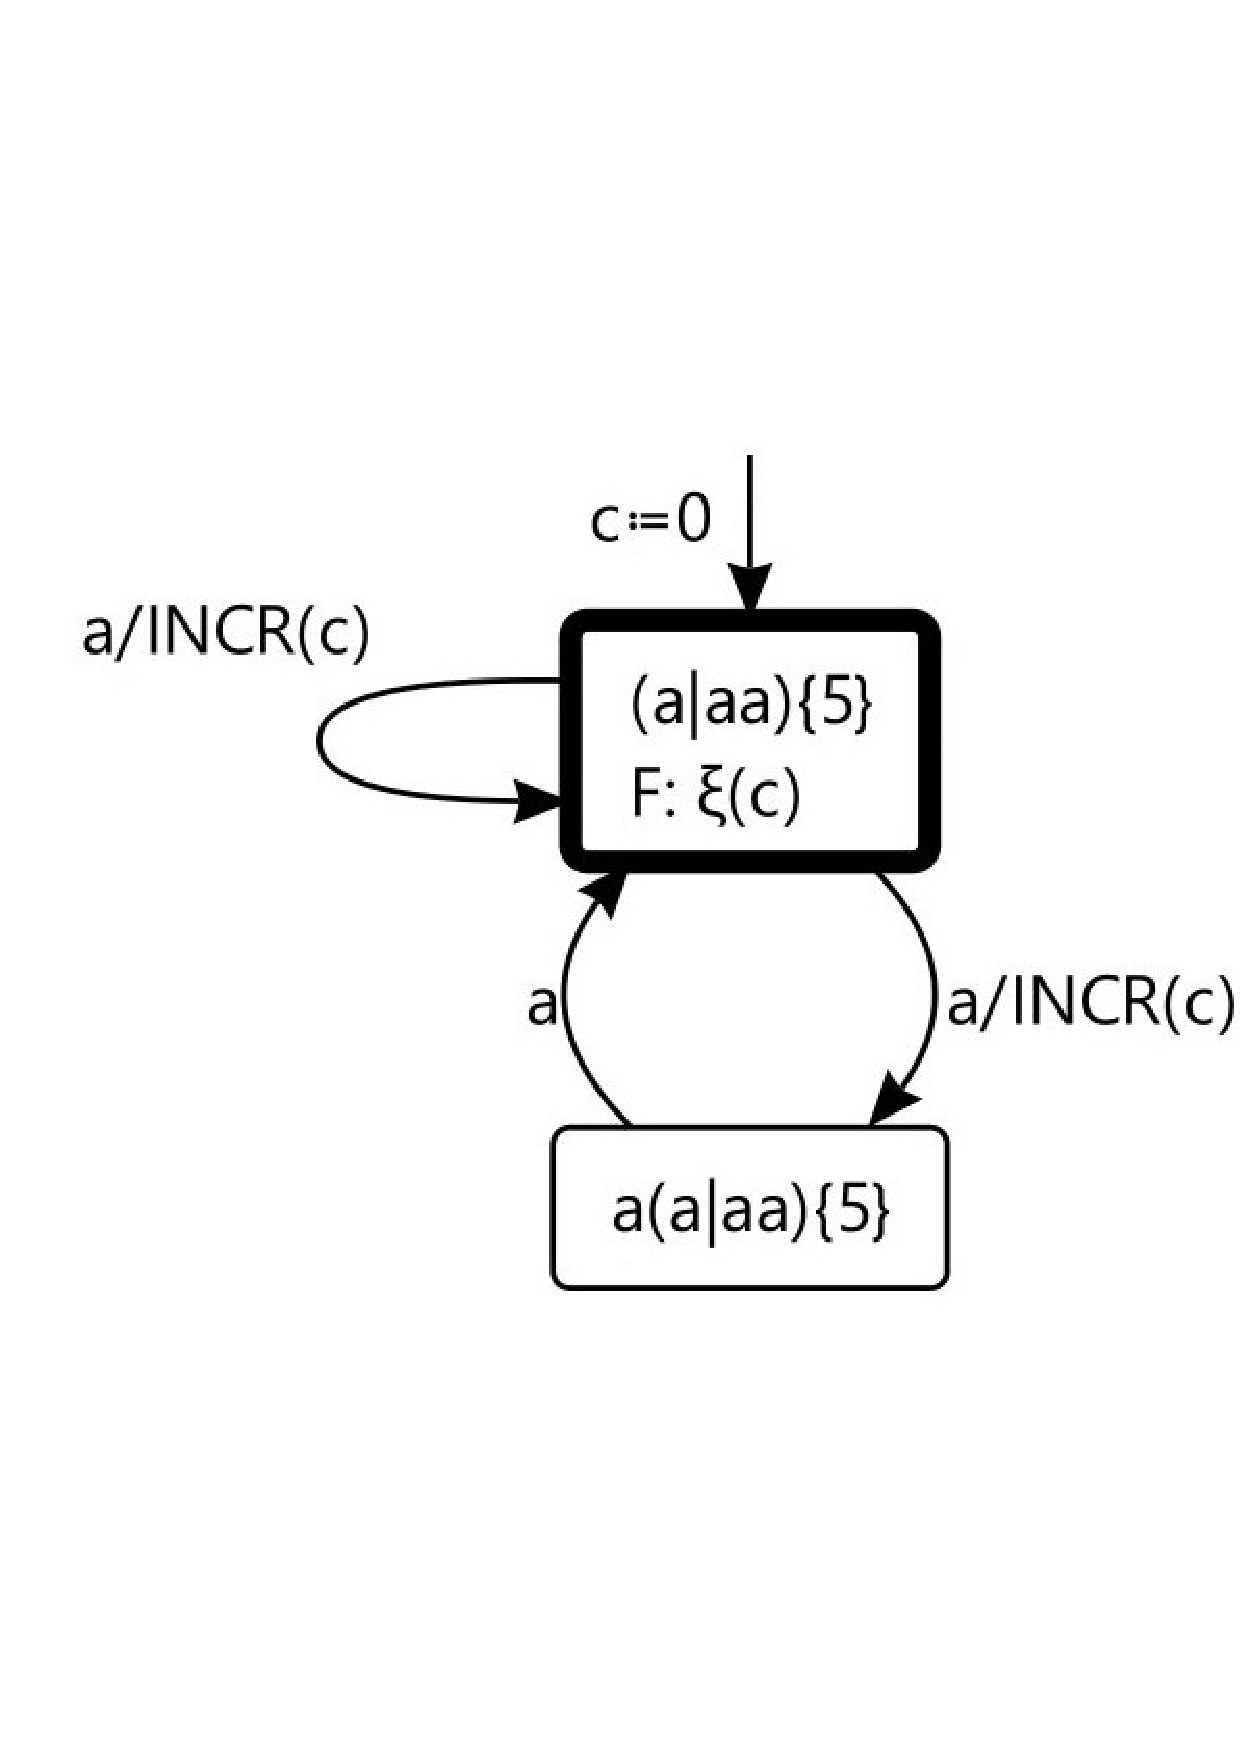
\includegraphics[width=3.7cm,trim=30 220 0 220,clip]{figures/aoraafive.pdf}}
%        \vspace*{-3mm}
%        \caption{$\mathit{CA}(\regex{(a|aa)\{5\}})$.\label{fig:aoraafive}}
%\end{wrapfigure}
%\noindent   
%After reading the word $aa$, $\DFAof{\CA(R)}$
%reaches the powerstate $\{(q_0,c=1),(q_0,c=2),(q_1,c=2)\}$,
%which is not Cartesian because both states are in the scope of the counter $c$
%but are paired with different counter values. Our CsA would reach the
%configuration $(\{q_0,q_1\},c\in\{0,1,2\})$, which encodes the larger powerstate
%$\{(q_0,c=0),(q_0,c=1),(q_0,c=2),(q_1,c=0),(q_1,c=1),(q_1,c=2)\}$ 
%where both states appear with both counter values.
%\qed
%\par}%
%\end{exnoqed}
%
%\cbstart
%%------------------------------------------------------------------------------
%\paragraph{Uniformity}
%%------------------------------------------------------------------------------
%
%We now introduce the so-called \emph{uniformity} of a CA as a property under
%which determinization preserves the language.
%%
%Uniformity prevents creation of non-Cartesian powerstates. 
%%
%It includes two conditions.
%
%The first condition prevents the kind of scenario from \cref{ex:noncartesian}.
%%
%For each DFA transition $\tau'$, it requires that every CA state $q$ that is in
%the scope of some counter $c$ within the DFA state to which $\tau'$ leads
%receives the same set of values of $c$. 
%%
%This requires testing whether the sets of transitions covered by $\tau'$ and
%incoming to every such CA state $q$ induce the same CsA operations~for~$c$. 
%
%The second condition prohibits two counters from being active at once, a
%scenario which arises from regexes with nested counting. 
%%
%Indeed, the relation between values of two simultaneously active counters may
%easily become more intricate than what can be expressed by a Cartesian product
%of two sets (consider, e.g., the regex $a?(a\{1\}a)\{2\}$ and the word $aaa$).
%%
%The condition requires testing that no state appears in the scope of two
%counters. 
%
%
%Formally, given a CsA transition $\tau' =
%\move{S}{\prodp{\alpha}{\beta},\CS{f}}{T}$, a~counter $c$, and a~CA state $q \in \scope(c)$,
%we define the set $\CS{f}_q(c)$ of \emph{incoming CsA operations} for $c$
%induced by the incoming transitions of $q$ from which $\tau'$ is built
%($\alpha$-transitions consistent with $\beta$ originating in $S$) as follows: 
%$$
%\CS{f}_q(c) \eqdef\{\textit{op}(\tau,c)\mid
%\tau\in 
%%\consistent(c) 
%\Delta_{S,\alpha, \beta(c)}
%\land \text{the target of $\tau$ is $q$}\} \ .
%$$
%We call the transition $\tau'$ \emph{uniform} iff, for each counter $c\in C$,
%any two states $q,r\in \scope(c)\cap T$ have the same sets of incoming CsA operations, i.e., $\CS{f}_q(c) = \CS{f}_r(c)$. 
%%
%The~\CA $\aut$ is then \emph{uniform} if all transitions of $\CS \aut$ are
%uniform and if no state of $A$ appears in the scope of two counters.
%
%\begin{theorem}
%  \label{thm:inv}
%  If a~\CA~$\aut$ is uniform, then 
%   $\langof{A}=\langof{\CS{A}}$.
%\end{theorem}
%\begin{proof}[Proof (idea)]
%  By showing bisimilarity between states $q$ of $\NFAof{\CS{A}}$, i.e.,
%  configurations of the CsA~$\CS{A}$ and powerstates $\pstateof q$ of $\DFAof{A}$. 
%\end{proof}
%
%Uniformity can be checked on the fly, while constructing $\CS{\aut}$. 
%%
%It is also automatically implied when the \CA is constructed from certain
%classes of regexes, as discussed below.
%\cbend
%
%%==============================================================================
%\subsection{Syntactic Correctness Criteria}\label{sec:syntcorrectness}
%%==============================================================================
%%\vspace{-0.5mm}
%
%Uniformity is only a~semantic property.
%%
%Below, we show examples of actual regexes that do and do not lead to uniform CAs
%and discuss some simple syntactic classes of regexes that imply uniformity.
%%
%A~detailed study of syntactic classes of regexes that guarantee uniformity is,
%however, beyond the scope of this paper and a~part of our future work. 
%
%The regexes that induce non-uniform CAs are often those where, intuitively,
%there is a position in some input text that may either be matched against the first
%character of a counted sub-expression or against some inner character of the
%same sub-expression.
%In such a~situation, there may be two runs of the induced CA: one that
%increments the associated counter (the increment happens) at that position and
%moves to some state~$q$, and the other that leaves the counter as it is, while
%in its scope, and moves into a different state~$r$. 
%The counter value then depends on the state: it is different in~$q$ and in~$r$.
%The corresponding DFA state is then non-Cartesian and the CA is non-uniform.
%
%%\vspace{-1mm}
%\begin{example}
%We present several commented examples of regexes with non-uniform CAs
%where our determinization overapproximates the language of the obtained CsA.
%\begin{itemize}
%\item 
%\regex{(a|ab|ba)\{5\}} --- the string $aba$ could be matched as~``\regex{a}''
%    followed by~``\regex{ba}'', having incremented the counter twice, or as
%    ``\regex{ab}'' that is followed by the prefix~``\regex{a}''
%    of~``\regex{ab}'', having incremented the counter once only.
%\item 
%\regex{a\{1,3\}a\{3\}} --- this case can be explained similarly as the previous
%one. Alternatively, note that, assuming that our translation to a CA produces
%two counters, say $c_1$ and $c_2$, then after reading $n$ letters $a$, the CA needs to remember that $c_1 + c_2 = n$. Such non-trivial relations between counter values are not Cartesian.
%\item
%\regex{\DOT*(aa)\{6\}} --- assuming a sequence of $a$'s on the input, the
%    counter may be either incremented on odd characters and left unchanged on
%    even ones, or the other way around.
%    As the counter values depend on the position within the ``\regex{aa}'' (and
%    hence on the CA state), the CA cannot be uniform. 
%Note that the prefix $\regex{\DOT*}$ is quite usual as it corresponds to searching
%for the regex $\regex{(aa)\{6\}}$ anywhere in the input string. 
%\item 
%\regex{\DOT*(a\{2\})\{2\}} --- after reading $aa$, if the value of the outer
%    counter is $1$, then the value of the inner counter must be $0$. This is a
%    non-trivial relation between the values of the two counters, which is not Cartesian.
%Nested counting is often problematic, however, many of such examples may still be solved quite efficiently by unfolding one of the counters.
%\qed
%\end{itemize}
%\end{example}
%
%%\vspace{-2mm}
%\paragraph{Syntactic classes of regexes that guarantee uniformity.}
%A simple class of regexes that guarantees uniformity is a generalization of the class of \emph{monadic} regexes of \cite{aplas19} (where
%counting is allowed over character classes only).
%%
%%Namely, the property required is that counting loops are of the form
%Namely, it includes regexes with counting loops of the form
%%\vspace{-0.5mm}
%$$
%\text{$(\alpha_1\ldots\alpha_n)\{\ell,k\}$ s.t. $\semof{\alpha_1}$ is disjoint from
%every $\semof{\alpha_i},1<i\leq n$.} 
%%\vspace{-0.5mm}
%$$
%%
%Intuitively, the disjointness with $\alpha_1$ ensures that the generated CA will
%only be able to process $\alpha_1$ through an increment transition at the
%beginning of a new iteration of the loop, with no possibility of having a
%conflicting $\NoOp$ transition that could read the same symbol inside the body
%of the loop (which is exactly what happens with the second symbol $a$ in
%\cref{ex:noncartesian}). The CsA compiled form this class are also guaranteed to be fast.
%
%%Nonetheless, the class of regexes where our determinisation preserves the language seems to be much
%%larger.
%%%
%%For instance, it includes the regexes \regex{((aa)|(bb))*aa((aa)|(bb))\{$k$\}} and
%%\regex{\DOT*((Natasha)|(Yurij)|(banza\{8\}j!))\{5\}}, despite that the
%%latter even uses nested counting.
%
%\newcommand{\plotfigure}[0]{
%\begin{figure}[t]
%\begin{subfigure}[b]{0.47\linewidth}
%\hspace*{-2mm}
%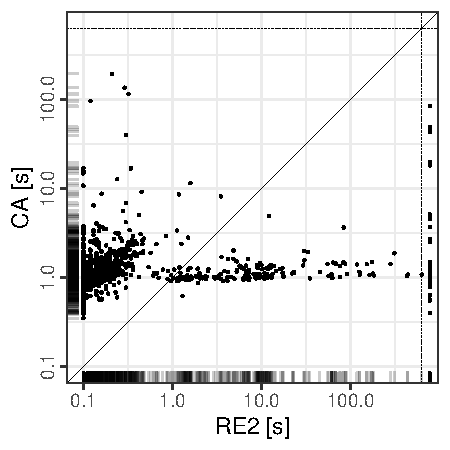
\includegraphics[width=6.7cm,keepaspectratio]{figures/re2g-vs-cad.pdf}\\
%\vspace*{-6mm}
%\caption{The comparison of running times of \catool and \retwo on our benchmark
%set (\catool wins: 287/1,789)}
%\label{fig:ca-vs-re2}
%\end{subfigure}
%\hfill
%\begin{subfigure}[b]{0.47\linewidth}
%\hspace*{-6mm}
%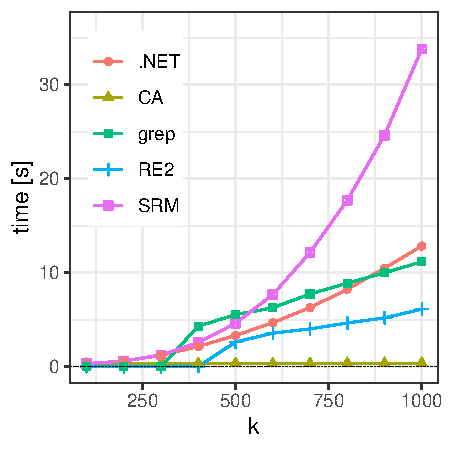
\includegraphics[width=6.7cm,keepaspectratio]{figures/big_plot-1000.pdf}\\
%\vspace*{-6mm}
%\caption{Running times of the tools on the regex ``\regex{(\_a )\{$k$\}\_a}''
%where~$k$ is a~parameter}
%\label{fig:increase}
%\end{subfigure}\\
%
%\newlength{\triplepiclen}
%\setlength{\triplepiclen}{4.5cm}
%\begin{subfigure}[b]{\linewidth}
%\begin{center}
%  \begin{minipage}{\triplepiclen}
%  \begin{center}
%    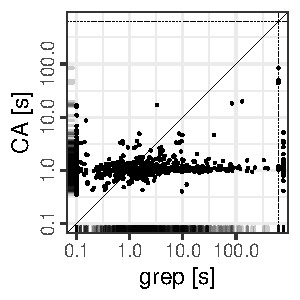
\includegraphics[width=1\triplepiclen,keepaspectratio]{figures/grep-vs-cad.pdf}\\
%    \hspace*{5mm}
%    (\catool wins: 862/1,425)
%  \end{center}
%  \end{minipage}
%  \begin{minipage}{\triplepiclen}
%  \begin{center}
%  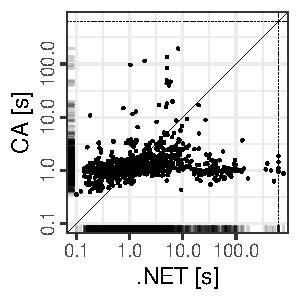
\includegraphics[width=1\triplepiclen,keepaspectratio]{figures/dotnet-vs-cad.pdf}\\
%    \hspace*{5mm}
%    (\catool wins: 708/1,789)
%  \end{center}
%  \end{minipage}
%  \begin{minipage}{\triplepiclen}
%  \begin{center}
%  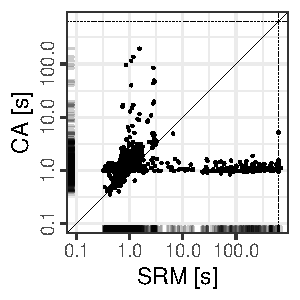
\includegraphics[width=1\triplepiclen,keepaspectratio]{figures/srm-vs-cad.pdf}\\
%    \hspace*{5mm}
%    (\catool wins: 345/1,789)
%  \end{center}
%  \end{minipage}
%\end{center}
%\caption{The comparison of running times of \catool with \grep, \dotnet, and \srm on our benchmark set}
%\label{fig:ca-vs-tools}
%\end{subfigure}
%
%\vspace*{-1mm}
%\caption{Graphs with results of our experiments.
%  Note that, in~(\subref{fig:ca-vs-re2}) and~(\subref{fig:ca-vs-tools}), the axes
%  are logarithmic, the dashed lines denote the timeout (600\,s), and
%  the data points between the dashed lines and the edge of a plot represent
%  benchmarks where the tool did not run successfully.
%  We also
%  provide the number of times \catool won.
%}
%\label{fig:graphs}
%\vspace{-3mm}
%\end{figure}
%}
%

%\vspace{-1mm}
%%%%%%%%%%%%%%%%%%%%%%%%%%%%%%%%%%%%%%%%%%%%%%%%%%%%%%%%%%%%%%%%%%%%%%%%%%%%%%%%
\section{Experimental Evaluation}\label{sec:experiments}
%%%%%%%%%%%%%%%%%%%%%%%%%%%%%%%%%%%%%%%%%%%%%%%%%%%%%%%%%%%%%%%%%%%%%%%%%%%%%%%
\vspace{-0.5mm}

We have implemented our approach in a C\#
prototype called \catool
available at~\blinded{\cite{chipmunk}}
%(see
%\ifTR
%\cref{sec:Implementation}
%\else
%\cite{OOPSLA20TR}
%\fi
%for details how to efficiently implement
%{\CSA}s)
and evaluated its capability of generating text causing 
 against other
state-of-the-art regex matchers on patterns that use the counting operator.
We focused on comparison against
Google's \retwo library~\cite{re2}%
\footnote{%
  We used the version 2019-01-01 of \retwo via the command line interface \texttt{re2g} from
  \url{https://github.com/akamai/re2g}.
}, an automata-based matcher designed to be fast, predictable, and resilient against ReDoS attacks.
We also include other three efficient matchers into the comparison, namely
the standard GNU \grep program~\cite{grep} (version~3.3),
the \dotnet standard library regex matcher from
\texttt{System.Text.RegularExpressions}~\cite{dotnet}, and
Symbolic Regex Matcher (\srm)~\cite{VSXW19}.

%Let us shortly summarize how the tools work.
%The main algorithms of
%\retwo and \grep implement optimized versions of the Thompson's on-the-fly
%determinization where the constructed DFA states are cached.
%The construction has a~bound on the size of the DFA---if the bound is reached,
%the so-far constructed DFA states are flushed to avoid consuming too much
%memory.
%In some situations when caching is found ineffectual, \retwo turns the caching
%off,
%and the performance can drop even lower 
% (see the description in~\cite{regexes-in-the-wild} for details).
%We note that \retwo rejects an input regex if it contains a~counting
%operator with a~bound bigger than 1,000.
%%
%\srm is based on \emph{symbolic derivatives} constructed on the fly, 
%also in the spirit of the Thompson's algorithm, and, likewise, bases its efficiency
%on caching
%(in fact, \srm is quite close to an implementation of the Thompson's
%algorithm over CAs with caching).
%The~\dotnet matcher uses a~backtracking algorithm over NFAs, while
%%
%our \catool eagerly constructs a~deterministic CsA for the input regex.
%%
%The former four are mature tools, and especially \retwo and \grep contain many high- and low-level
%optimizations, such as using the Boyer-Moore algorithm~\cite{BoyerM77} to skip
%over many characters that are known to not be a~part of a~match.
%%
%\retwo and \grep are compiled programs while \catool, \srm, and
%\dotnet run within the .NET Framework (therefore, they have some inherent
%overhead due to the \emph{just-in-time} compilation at start-up and its
%inability to use advanced code optimizations, as well as 
%garbage collection). 
%%
%Note that even though the tools based on the on-the-fly subset construction (\retwo, \grep, and \srm) are linear to the lenght of the text, they still take space exponential to the counter bounds in the worst case, by creating sets of the size linear to the counter bounds, exponential to their decadic encoding used in the regex. 
%
%We run our benchmarks on a~machine with the Intel(R) Xeon(R) CPU E3-1240 v3 @
%3.40\,GHz running Debian GNU/Linux (we use the Mono
%platform~\cite{mono} to run .NET~tools).
%To avoid issues with generating exact matches,
%which might differ for different tools,
%the tools were run in the setting where they counted the number of lines
%matching\footnote{%
%We consider the standard semantics of ``matching'' used by \texttt{grep}, i.e.,
%a~line matches a~regex~$R$ if it contains a~string that is in~$\langof R$, unless it
%contains start-of-line (\texttt{\^}) or end-of-line (\texttt{\$}) anchors, in which
%case the matched string needs to occur at the start and/or at the end of the
%line respectively.
%}
%\mbox{the given regex (e.g.\ the \texttt{-c} flag of \grep).}


%
%\plotfigure
%
%%*******************************************************************************
%\vspace{-0.0mm}
%\subsection{ReDoS Resiliency}\label{sec:exp_redos}
%\vspace{-0.0mm}
%%*******************************************************************************
%Our main experiment focuses on the resilience of the matching engines
%against ReDoS attacks.
%The regexes used for this experiment were selected (1) from the database of over
%500,000 real-world regexes coming
%%
%from an Internet-wide analysis of regexes collected from over 190,000 software
%projects~\cite{DavisMCSL19}; 
%(2) from databases of regexes used by \emph{network intrusion detection systems} 
%(NIDSes), in particular, Snort~\cite{snort},
%Bro~\cite{bro},
%Sagan~\cite{sagan}, and the academic
%papers~\cite{yang2010,tacas18-appred};
%(4) the RegExLib database of regexes~\cite{regexlib}; and
%(5) industrial regexes from~\cite{aplas19}, used for security purposes.
%\mbox{From these, we created our set of benchmarks by the following steps:}
%%
%\begin{enumerate}[(1)]
%  \item  We selected regexes that contained counting loops whose
%    sum of upper bounds was larger than~20.
%    This let us focus on regexes where the use of counting makes
%    sense (there are surprisingly many regexes occurring in practice where the
%    use of a~counting loop is unnecessary, e.g., regexes containing
%    sub-expressions similar to \regex{a\{0,1\}} or even just \regex{a\{1\}}).
%    Moreover, we also removed all except 26 regexes with counters bigger than
%    1,000, which cannot be handled by \retwo.
%    We left the 26 regexes as representatives of ``large'' counters.
%    This left us with 5,000 regexes.
%\cbstart
%  \item  Then, we filtered out regexes~$R$ such that either $\CA(R)$ was not uniform 
%   (i.e., the \CSA produced by our algorithm was not precise, cf. \cref{sec:correctness}), 
%   or such that the $\CSA$ was not fast 
%   (i.e. not all counting-set operators were constant-time, cf. \cref{sec:CsA}).
%    After this step,
%    a vast majority,
%    4,429 
%    of the regexes, remained. 
%\cbend
%  \item  For the regexes that remained, we used a~lightweight ReDoS generator designed to
%    exploit counting (cf.~\cref{sec:redos_gen}) to generate $\sim$10\,MiB long
%    input texts.
%    In particular, we managed to generate ``adversarial'' input texts for
%    1,789 
%    regexes (for the rest of the regexes, either the underlying state space was
%    too small, so the generator could not construct the text, or the generation hit the
%    timeout of 600\,s).
%    Our benchmark data set is available at~\cite{oopsla20-dataset}.
%\end{enumerate}
%%
%We ran all tools on the generated benchmarks (counting the number of lines of
%the input text matching the regex) and give scatter plots comparing the running
%times of the tools in \cref{fig:ca-vs-re2} and \cref{fig:ca-vs-tools} (the
%timeout was 600\,s).
%On the bottom and the left-hand side of every plot, there are rug plots
%illustrating the distribution of the data points.
%Note that the axes are logarithmic, so the difference between data points grows
%as these points are away from zero (in particular, differences of values
%smaller than 1\,s are negligible).
%The semantics of regexes supported by \grep differs from the one
%supported by other tools, so we only considered the
%cases when the number of matches was the same when comparing with \grep).
%In the plots, the data points between the dashed lines and edges of the plots
%represent errors, e.g. due to the regex being rejected (for counters $>$1,000 for
%\retwo) or being interpreted using a different semantics (in the case of \grep).
%
%\begin{table}[t]
%\footnotesize
%% \vspace*{-7mm}
%\caption{Statistics for the graphs in \cref{fig:graphs} (times are given in seconds).
%For \catool, we provide several times:
%``total'' is the total time,
%``CA'' is the time for translating a regex into a (nondeterministic) CA,
%``CsA'' is the time of determinization of the CA into a CsA, and
%``match'' is the time spent when matching the input text.
%}
%\vspace*{-2.5mm}
%\begin{center}
%%latex.default(desc, file = "figs/stats.tex", booktabs = TRUE,     table.env = FALSE, center = "none")%
\begin{tabular}{lrrrrrrrr}
\toprule
                   & \multicolumn{1}{c}{\retwo} & \multicolumn{1}{c}{\grep} & \multicolumn{1}{c}{\dotnet} & \multicolumn{1}{c}{\srm} & \multicolumn{4}{c}{\catool}  \tabularnewline
                   &                            &                           &                             &                          & total                                        & CA & CsA & match \tabularnewline
\midrule
mean      & $   36.11$ & $   34.38$ & $    9.12$ & $   26.78$ & $   1.73$ & $0.05$ & $0.23$ & $0.69$ \tabularnewline
median    & $    0.10$ & $    0.70$ & $    0.76$ & $    0.73$ & $   1.03$ & $0.03$ & $0.04$ & $0.68$ \tabularnewline
std.\ dev & $  157.05$ & $  147.17$ & $   52.10$ & $  106.16$ & $   7.27$ & $0.29$ & $2.73$ & $0.29$ \tabularnewline
timeouts  & 1          & 11         & 8          & 16         & 0         &        &        & \tabularnewline
\bottomrule
\end{tabular}

%\end{center}
%\label{tab:stats}
%\vspace{-2.0mm}
%\end{table}
%
%In \cref{fig:ca-vs-re2}, we compare \catool with \retwo.
%We wish to point out the following interesting observations.
%Although \retwo wins more often  on the whole benchmark set 
%(our prototype does not include the many
%advanced optimizations present in \retwo),
%there is
%a~number of benchmarks (287)\ where its performance significantly deteriorates,
%and \catool is faster.
%In particular, there are 89 benchmarks where the time of \retwo is bigger than
%10\,s, i.e., its speed drops below~1\,MiB/s (we consider this speed of
%processing denotes a successful ReDoS attack, even though the limit may be
%significantly larger in practice\footnote{%
%  The required processing speed depends on the application.
%  NIDSes performing deep packet inspection may require a line-processing speed of
%  units or tens of GiB/s~\cite{tacas18-appred}, while application servers
%  validating user inputs may suffice with units or tens of MiB/s.
%}).
%For \catool, the number of benchmarks that took over 10\,s was only~22; 
%in fact, all except
%3~benchmarks finished within 100\,s---the blow-up in these 3~benchmarks is not caused by the
%counters but rather by many ``\regex{|}'' and ``\regex{?}'' operators, so over
%70\,\% of the total time is spent by constructing the \CSA.
%If~used, e.g.,\ in an NIDS, the \CSA would be created only once and then used
%for matching giga-/terabytes of data, so the initial overhead could be neglected.
%
%%!!!!!!!!!!!!!!!!!!!!!!!!!!!!!!!!
%%\enlargethispage{2mm}
%%!!!!!!!!!!!!!!!!!!!!!!!!!!!!!!!!
%
%
%Comparing with the other tools (\cref{fig:ca-vs-tools}) and also clearly visible 
%in the corresponding rug plots and the statistics in
%\cref{tab:stats},
%we can observe that the performance of \catool is much more robust than
%the performance of the other tools;
%the mean time and standard deviation of \catool is significantly lower than the
%rest of the tools.
%In particular, from the benchmarks where \catool was faster than \retwo, the
%time of \catool on all except two benchmarks was almost the same (including
%them, the standard deviation was 0.37).
%We provide four times for \catool:
%``total'': the total user time of matching (measured using the GNU \texttt{time} utility),
%``CA'': the time for translating the input regex into a~CA,
%``CsA'': the time it took to determinize the CA into a~CsA, and
%``match'': the time of matching the input text with the CsA.
%Note that, in the tables, there is a~noticeable discrepancy between the sum
%$\text{``CA''} + \text{``CsA''} + \text{``match''}$ and ``total'', which is
%due to the .NET Framework overhead, such as just-in-time compilation and (in
%particular) the garbage collector.
%
%In \cref{tab:best_results}, we give a~selection of interesting benchmarks.
%These contain benchmarks that are difficult for usually more than one tool.
%We emphasize the benchmarks coming from the NIDSes Snort and Bro.
%Notice that, for most of them, matching using \retwo (and also other tools) gets
%extremely slow.
%Slow matching over these regexes can have disastrous consequences for network
%security, potentially completely eliminating a~given NIDS.
%
%\newcommand{\LF}{Sw}
%
%\newcommand{\interestingtable}[0]{
%\begin{table}[t]
%\footnotesize
%\caption{Selection of interesting benchmarks. ``\timeout'' denotes a~timeout
%(600\,s) and ``---'' denotes an error.
%Due to space constraints, in the ``Regex'' column, ``\ldots'' denotes omitted
%parts of the regexes (we tried to preserve the parts containing occurrences of
%  the repetition operator) and
%``\recont'' denotes breaking a regex into two lines. 
%In the column source, \LF\ denotes the regexes collected in \cite{DavisMCSL19} from software projects. 
%}
%% \vspace*{-3mm}
%\label{tab:best_results}
%\vspace*{-2.5mm}
%\begin{center}
%{
\setlength{\tabcolsep}{4pt}
%\newcommand{\closer}{\hspace{2.5mm}}
%\begin{tabular}{llr@{\closer}r@{\closer}r@{\closer}r@{\closer}r@{\closer}r@{\closer}r@{\closer}r}
\begin{tabular}{llrrrrrrrr}
\toprule
\multicolumn{1}{c}{Source\hspace*{-3mm}} & \multicolumn{1}{c}{Regex}                                                                             & \multicolumn{1}{c}{\retwo} & \multicolumn{1}{c}{\grep} & \multicolumn{1}{c}{\dotnet} & \multicolumn{1}{c}{\srm} & \multicolumn{4}{c}{\catool} \tabularnewline
                                         &                                                                                                       &                            &                           &                             &                          & total                                       & CA              & CsA     & match \tabularnewline
\midrule
\mrtwo{Snort}                            & \verb#.*[aA][uU][tT][hH]#\ldots\verb#[iI][cC] #\recont                                                                & \mrtwo{$11.27$}                    & \mrtwo{$7.8 $}                    & \mrtwo{$361.1$}                     & \mrtwo{$555.56$}                 & \mrtwo{$1.04$}                                      & \mrtwo{$0.03$}          & \mrtwo{$0.05$}  & \mrtwo{$0.31$} \tabularnewline
                                         & \recont\verb#[^\x0A]{512}#\\
Snort                                    & \verb@\x20[^\x21\x22]{500}@                                                                           & $439.98$                   & $  0.11$                  & $  2.20$                    & \timeout                 & $1.08$                                      & $0.03$          & $0.04$  & $0.83$ \tabularnewline
\mrtwo{Snort}                            & \verb#^RCPT TO\x20\s*[\w\s@\.]{200,}#\recont                                                          & \mrtwo{$340.7$}                    & \mrtwo{---}                       & \mrtwo{\timeout\!\!}                    & \mrtwo{\timeout\!\!}                 & \mrtwo{$1.68$}                                      & \mrtwo{$0.03$}          & \mrtwo{$0.07$}  & \mrtwo{$0.89$} \tabularnewline
                                         & \recont\verb#\x20[\w\s@\.]{200,}#\ldots \\
Snort                                    & \verb#php.*\x20[^\n]{256}#                                                                            & $176.75$                   & $  0.10$                  & $  1.22$                    & \timeout                 & $1.08$                                      & $0.04$          & $0.07$  & $0.74$ \tabularnewline
\mrtwo{Snort}                            & \verb#^(NT|CallBack|SID|TimeOut)\s*#\recont                                                           & $164.11$                   & $  0.12$                  & $ 14.59$                    & $229.41$                 & $1.07$                                      & $0.03$          & $0.07$  & $0.72$ \tabularnewline
                                         & \recont\verb#\x20\s*[^\n]{512}#\\
Snort                                    & \verb#.*[nN][eE][wW]#\ldots\verb# [^\x20]{100}#                                                       & $0.13 $                    & $1.26$                    & $39.92$                     & $0.74  $                 & $0.81$                                      & $0.03$          & $0.04$  & $0.65$ \tabularnewline
\mrtwo{Bro}                              & \verb#^[nN][aA][mM][eE]=s*[^\r\n\x3b#\recont                                                          & \mrtwo{$128.57$}                   & \mrtwo{$ 12.24$}                  & \mrtwo{$  0.51$}                    & \mrtwo{$ 76.48$}                 & \mrtwo{$1.15$}                                      & \mrtwo{$0.03$}          & \mrtwo{$0.04$}  & \mrtwo{$0.94$} \tabularnewline
                                         & \recont\verb#\x20\x09\x0b\x2c]{300}# \\
\LF                        & \verb#_.{39}#                                                                                         & $22.96$                    & $225.34$                  & $1.94$                      & $357.68$                 & $1.12$                                      & $0.03$          & $0.04$  & $0.79$ \tabularnewline
\LF                        & \verb#(.{1,980}[,])\s+(\S)#                                                                           & $260.59$                   & \timeout                  & $308.66$                    & $  0.63$                 & $1.07$                                      & $0.03$          & $0.05$  & $0.59$ \tabularnewline
\LF                        & \verb#(_a ){64999}_a#                                                                                 & ---                        & ---                       & \timeout                    & \timeout                 & $0.96$                                      & $0.03$          & $0.04$  & $0.51$ \tabularnewline
\LF                        & \verb#\[{50000}a\]{50000}#                                                                            & ---                        & ---                       & $4.36 $                     & \timeout                 & $5.13$                                      & $0.02$          & $0.02$  & $0.41$ \tabularnewline
\mrtwo{\LF }               & \verb#^QS([NDR])(.{4})(.{6})(\d{8})#\ldots\recont\hspace*{-3mm}                                       & \mrtwo{$0.12$}                     & \mrtwo{$0.10$}                    & \mrtwo{$1.03$}                      & \mrtwo{$0.85$}                   & \mrtwo{$96.20$}                                     & \mrtwo{$0.04$}          & \mrtwo{$81.64$} & \mrtwo{$0.65$} \tabularnewline
                                         & \recont\verb#(.{4})(.{6})(.{8})(.{8})(.)$# \\
\bottomrule
\end{tabular}
}

%\end{center}
%\vspace*{-2.0mm}
%\end{table}
%}
%
%The {\CSA}s produced by \catool were also much smaller than the corresponding DFAs.
%%
%The CsAs have on average 29 states (median: 7) and 306
%transitions (median: 11).
%%
%On the other hand, classical NFAs constructed from the regexes have on average 112 states (median: 52),
%%
%and when determinized, the resulting DFAs have on average 2,802 states
%(median: 67) and 10,384 transitions (median: 107).
%%
%Using {\CSA}s significantly lowers the chance that determinization
%explodes.
%
%%-------------------------------------------------------------------------------
%%\vspace{-1.0mm}
%\subsubsection{The Effect of Nondeterministic Counting}\label{sec:label}
%\vspace{-0.0mm}
%%-------------------------------------------------------------------------------
%We say that a~regex contains \emph{nondeterministic counting} if, when
%translated into a~CA~$A$ using the algorithm in \cref{sec:regexes}, there is
%a~word~$w$ such that~$A$ can over~$w$ reach two configurations with different
%values of some counter.
%
%Regexes with nondeterministic counting are the main focus of our benchmark.
%Namely, they constitute 67\,\% of the 1,789 regexes used.
%From the 1,284 regexes that were at least \emph{slightly} problematic for some of
%the other tools except \catool (it took some tool $\geq$ 1\,s),
%73\,\% of them were with nondeterministic counting.
%From the 454 regexes that were \emph{significantly} problematic for some of the other
%tools (it took some tool $\geq$ 10\,s), 85\,\% of them had
%nondeterministic counting.
%From the 109 regexes that were \emph{problematic} for \emph{all} other tools ($\geq$
%1\,s), 100\,\% were with nondeterministic counting.
%As shown in the results above, our approach can deal with
%nondeterministic counting quite well.
%
%
%%-------------------------------------------------------------------------------
%%\vspace{-1.0mm}
%\subsubsection{Adversarial Regexes}
%\vspace{-0.0mm}
%%-------------------------------------------------------------------------------
%Another ReDoS scenario is when the attacker can control the regex to be used for
%matching.
%%
%Creating a~counting regex causing efficiency problems for a~given text
%is easier than generating adversarial texts.
%For instance, the regex
%\texttt{[a-zA-Z().,'\ ]*[a-zA-Z\ ] [a-zA-Z()\.,'\ ]\{250\}} was obtained as
%a~modification of the running example ``\regex{\DOT*a\DOT\{$k$\}}'' (where \regex{a} appears
%$k$ positions from the end).
%When run on a $\sim$4\,MiB English text with sufficiently long lines,
%\retwo took 86\,s, \grep took 26\,s, while \catool took only~1.1\,s.
%Similar examples could be obtained from regexes from \cref{sec:exp_redos} for which some specific difficult text can be generated, namely by widening their character classes.. 
%Our approach solves a large class of the dangerous cases,
%allowing one to significantly alleviate restrictions put on the user for 
%security/efficiency reasons.
%
%%*******************************************************************************
%\vspace{-1.0mm}
%\subsection{Robustness wrt\ Counter Values}\label{sec:label}
%\vspace{-0.5mm}
%%*******************************************************************************
%%!!!!!!!!!!!!!!!!!!!!!!!!!!!!!!!!
%\enlargethispage{2mm}
%%!!!!!!!!!!!!!!!!!!!!!!!!!!!!!!!!
%
%
%\interestingtable
%This experiment measures the ability of the tools to cope with
%increasing counter bounds.
%For this, we selected the regex ``\regex{(\_a )\{$k$\}\_a}'' where~$k$ is a~parameter
%(the original regex \regex{(\_a )\{64999\}\_a} comes from~\cite{DavisMCSL19})
%and measured the time the tools took on a~$\sim$500\,KiB text created by our
%generator for increasing values of~$k$.
%\mbox{We give the results in \cref{fig:increase} (the timeout was 40\,s).}
%
%With the increasing value of~$k$, the time needed by \catool stays constant,
%around 0.35\,s,
%while the time needed by other tools grows.
%In particular, \dotnet and \srm have cubic trends wrt the value of
%$k$, while \retwo and \grep grow linearly.
%Notice that, for \retwo and \grep, their matching time is low (around 0.01\,s)
%until they reach a~threshold from which they start behaving linearly.
%This corresponds to the situation when the size of the cache for storing states
%of the NFA-to-DFA construction is not enough to accommodate the DFA states
%exercised by the input adversarial text.
%This yields repeated flushing of the cache, making it ineffectual.
%
%%*******************************************************************************
%%\vspace{-1.0mm}
%\subsection{Adversarial Text Generation}\label{sec:redos_gen}
%%\vspace{-0.5mm}
%%*******************************************************************************
%%\enlargethispage{1.5mm}
%
%\retwo and \grep store powerstates of the NFA-to-DFA construction in a cache.
%In typical cases, the amount of cache misses is low and almost the entire text
%is processed using the cache, which is extremely fast.
%If the cache, however, exceeds a given size, it is flushed.
%If the input text is such that the DFA run sees many different states, then
%cache misses are frequent, so large powerstates need to be constructed often, and
%the performance of the matching drops.
%
%Therefore, we focus on generating texts that force exploration of many new large
%powerstates. 
%In essence, we explore the configuration space of the \CSA with the goal of
%finding as many large configurations as possible, with the focus on generating
%large counting sets.
%We partially drive the search towards loops in the \CSA structure that have a
%potential to create large counting sets: the loops use counters with large bounds, do
%not contain exits, and contain $\ExitCSOp{}$ or $\ExitIncrCSOp{}$ operations.
%For space reasons, we omit the technical details here; perfecting
%this method for stress testing automata-based matchers is, however, one of our future
%goals.
%
%
%%*******************************************************************************
%%\vspace{-0.7mm}
%\subsection{A Note on the Maturity of the Tools}\label{sec:label}
%%\vspace{-1.0mm}
%%*******************************************************************************
%%%%%%%%%%%%%%%%%%%%%%%%%%%%%%%%%%%%%%%%
%%\enlargethispage{2mm}
%%%%%%%%%%%%%%%%%%%%%%%%%%%%%%%%%%%%%%%%
%
%The aim of our experiments is comparing algorithms rather than tools, and it should
%be noted that \catool is much less optimized than the rest.
%This holds especially for \retwo and \grep, which have both been actively
%developed for over 10 years and the amount of engineering effort invested into
%making them fast is substantial.
%%
%The optimizations are both high-level, such as using the Boyer-Moore algorithm
%for skipping sections of the input text, and low-level, such as using C/C++,
%on-the-fly determinization, or optimizing memory accesses~\cite{regexes-in-the-wild,
%why-gnu-grep-is-fast}. 
%%
%On the other hand,
%although there have been some optimizations done in 
%\catool (such as finding a~start of a~match), their nature is still quite
%simple.
%The three tools are, however, all based on the same principle of using
%deterministic automata, and many of the optimizations
%and heuristics in \retwo and \grep (at least all of those mentioned above) could
%be directly re-applied in our setting.
%\srm builds on the .NET framework and reuses the \dotnet regex parser
%while replacing the built-in backtracking back-end matcher with a
%matching engine based on Brzozowski-style symbolic derivatives to create
%the DFA on the fly.
%In fact, \catool builds on the open-source codebase of \srm and extends it with counters.
%
%
%%%%%%%%%%%%%%%%%%%%%%%%%%%%%%%%%%%%%%%%%%%%%%%%%%%%%%%%%%%%%%%%%%%%%%%%%%%%%%%%%
%%\vspace{-0.4mm}
%\section{Related Work}\label{sec:related}
%%\vspace{-1.0mm}
%%%%%%%%%%%%%%%%%%%%%%%%%%%%%%%%%%%%%%%%%%%%%%%%%%%%%%%%%%%%%%%%%%%%%%%%%%%%%%%%%
%
%%------------------------------------------------------------------------------
%\paragraph{Regexes and their derivatives.}
%%------------------------------------------------------------------------------
%
%Brzozowski derivatives~\cite{Brzozowski64_derivatives} provide a practical
%approach to incrementally creating a DFA from a regex and can be used for
%efficient matching~\cite{Owens09,Fis10} and match generation~\cite{VSXW19}.
%%
%Efficient determinization based on Brzozowski derivatives was first investigated
%in~\cite{BeSe86}.
%%
%In the classical setting, Antimirov
%derivatives~\cite{Antimirov96_partderivatives} are used to construct NFAs from
%regexes, and may in some cases result in exponentially more succinct automata
%than the corresponding DFAs constructed with Brzozowski derivatives.
%%
%The precise connection between conditional derivatives defined in
%Section~\ref{sec:regexes} and Antimirov derivatives is that, without counting
%loops,% $\RESET{R}\neq\emptyset$ \lt{$\RESET{R}$ or RST?} iff $R$ is nullable in the classical sense, and
%$\{D\mid \pair{\id}{D}\in\CD{a}{S}\}$ is exactly the Antimirov derivative of
%$R$ for $a$.
%%
%The Antimirov construction has also been generalized to extended regexes
%\cite{Champarnaud11_extended} allowing Boolean operators such as complement and
%intersection.
%%
%Basic theoretical properties between various automata formalisms and derivatives
%are discussed in \cite{Allauzen06_unified}.
%
%%\vspace{-0.5mm}
%%------------------------------------------------------------------------------
%\paragraph{Automata with counting.}
%%------------------------------------------------------------------------------
%This work is a continuation of our recent work~\cite{aplas19}.
%%
%In~\cite{aplas19}, we propose a~general determinization of CAs that can
%produce smaller automata than the naive explicit determinization but has the
%same worst-case complexity, which depends on the counters with the factor
%$(K+1)^{|C|}$ where $C$ is the set of counters and $K$ the maximum counter upper
%bound.
%%
%It also proposes a more efficient algorithm for the class of monadic regexes (single-state-scoped counters and counting on self-loops only), 
%but it can still generate $(K+1)^{|Q|}$ states 
%(for example, it would generate $K+1$ states for the regex from Fig.~\ref{fig:ak})---while the complexity of our determinization does not depend on $K$.
%%
%\cite{aplas19} also present neither a derivative construction for translating regexes into CAs nor 
%an application of CAs in pattern
%matching.
%
%The use of counters has also been investigated in~\cite{cikm15} for
%regexes with bounded repetition, building on the
%formalism of counter automata called CNFAs~\cite{GGM12}. 
%%
%A~CA in the current paper is essentially a~symbolic generalization of a CNFA
%with some small technical differences, such as counters being 0-based as opposed
%to 1-based in a~CNFA.
%The latter difference is mainly due to our use of
%a~generalized \emph{Antimirov} construction of CAs, 
%as opposed to a~generalized \emph{Glushkov} construction used
%in~\cite{GGM12}, which is algorithmically quite different.
%%
%The work in~\cite{cikm15} focuses mostly on deterministic regexes and on
%a~different problem, namely, the so-called incremental matching in the context
%of database queries (a~query is repeatedly evaluated on a gradually changing
%word).
%%
%For standard matching, it uses a variant of the Thompson's algorithm applied
%directly on a~CA instead of an NFA (hence the translation of the regex to an
%automaton does not depend on the counter bounds, but each text character
%is processed with the same cost as with the original Thompson's algorithm, at
%worst linear to the size of the NFA and the counter bounds).
%This algorithm is indeed fast on deterministic regexes from practice but can
%slow down significantly on nondeterministic ones (which we witnessed in several
%experiments with the prototype implementation of~\cite{cikm15} on several of our
%regexes).
%
%The work in \cite{KT03} is a theoretical study of matching regexes with
%counting. It proposes a matching algorithm based on dynamic programming that
%runs in time at worst quadratic to the length of the text (while determinization
%and NFA-simulation-based algorithms run in time linear to the text length). The
%experimental comparison of \cite{cikm15} with their variant of Thompson's
%algorithm suggests that the matching algorithm of \cite{KT03} is indeed not
%competitive in practice.
%
%Extended FAs (XFAs) augment classical automata with a scratch memory of
%bits~\cite{SEJ08,jha_extended} that can represent counters.
%%
%Regexes are compiled into deterministic XFAs by first using an extended version
%of the Thompson's algorithm, followed by an extended version of the
%classical powerset construction and minimization.
%%
%Although a small XFA may exist, the determinization algorithm incurs an
%intermediate exponential blowup of the search space for inputs such as
%\regex{\DOT*a\DOT\{$k$\}}.
%
%$R$-automata \cite{abdulla_rautomata} are also related to our CAs, but their
%counters need not have upper bounds and cannot be tested or compared.
%%
%Further, there are various notions of extended finite state machines whose
%expressive power goes beyond regular languages,
%e.g.,~\cite{cheng_efsm,shiple_efsm,jha_extended,finkel_fast}.
%%
%Such automata are, however, not suitable for the problem of pattern matching
%considered here.
%
%%!!!!!!!!!!!!!!!!!!!!!!!!!!!!!!!!
%%\enlargethispage{2mm}
%%!!!!!!!!!!!!!!!!!!!!!!!!!!!!!!!!
%
% 
%%\vspace{-1mm}
%%------------------------------------------------------------------------------
%\paragraph{Regexes with counting.}
%%------------------------------------------------------------------------------
% 
%Regexes with counters are also discussed
%in~\cite{Hovland09,KilTuh07,GMN07}.
%%
%The automata with counters used in~\cite{Hovland09}, called FACs, are close to
%our CAs, but we allow symbolic character predicates and more kinds of counter
%updates.
%%
%The conversion from regexes to FACs proposed in~\cite{Hovland09} uses a variant
%of Glushkov automata~\cite{Glu61} and the \texttt{first-last-follow}
%construction~\cite{BP96,BW98}.
%%
%For us, the Antimirov-derivative-based construction was easier to implement and
%provides benefits that are not available otherwise.
%%
%Namely, it allows subsumption checking between regexes,
%%
%and it generates fewer counters (one per distinct counter
%subexpression rather than one per counter position in the regex abstract syntax
%tree).
%%
%While all these algorithms generate $\epsilon$-free automata, they
%differ in complexity~\cite{Allauzen06_unified} and are thus not merely
%different disguises of the same technique.
%%
%In particular, the Antimirov automaton is in general smaller than the Glushkov
%automaton with up to $n+1$ states and up to $n^2$ transitions.
%%
%The Antimirov automaton is in fact a quotient of the Glushkov
%automaton 
%~\cite{CZ01,IlieYu03}.
%%
%Another generalization of Antimirov derivatives
%\cite{LOMBARDY2005141} introduces expressions $kR$ where $R$ is
%a~rational expression and $k$ a~multiplicity from a semiring such as
%$\mathbb{Q}$; this generalization is unrelated to counters.
% 
%An open question is whether the generalized Antimirov construction can be
%extended to work with Brzozowski derivatives~\cite{Brzozowski64_derivatives}; we
%believe that such an extension, if it exists, is not straightforward because it
%would give rise to a direct and incremental determinization algorithm.
% 
%There are also works on regexes with counting that translate
%deterministic regexes to CAs and work with different notions of
%determinism~\cite{GGM12,Chen15_counting}.
%%
%A central result in~\cite{Hovland09} is that \emph{counter-1-unambiguous}
%regexes can be compiled into deterministic FACs and that checking
%determinism of FACs can be done in polynomial time.
%%
%The related work in~\cite{Hovland-Membership2012} studies membership in regexes
%with counting.
%%
%None of these papers addresses the problem of determinizing nondeterministic
%CAs.
% 
%%\enlargethispage{2mm}
%%\vspace{-1mm}
%\vspace{-0.5mm}
%%------------------------------------------------------------------------------
%\paragraph{Pattern matching of regexes with counting.}
%%------------------------------------------------------------------------------
%
%The counting operator often appears in regexes in practice.
%%
%In particular, our analysis of the 537k real-world regexes obtained in the study
%performed by Davis et al.~\cite{DavisMCSL19} showed that over 33k regexes
%contained the counting operator.
%
%GNU \grep~\cite{grep} (written in C) and \retwo~\cite{re2} (written in C++) are
%extremely optimized regex matchers.
%%
%Both are based on translating the regex into an NFA and performing an on-the-fly
%determinization during the matching, avoiding a~costly \emph{a~priori}
%determinization,
%while keeping a~good performance by avoiding backtracking. (The translation into
%FAs is only allowed when the regex does not include back-references, which allow to express some context-free propeties).
%%provide the power to express some context-sensitive languages.)
%%
%Both engines process the counting operator by first rewriting a regex of the
%form \regex{<re>\{$n,m$\}} into \regex{<re>\ldots<re><re>\{0,$m-n$\}}.
%%
%The regex \regex{<re>\{0,$k$\}} is then transformed into
%\regex{(<re>(<re>(\ldots<re>?)?)?)?}
%%
%%More details about the DFA construction can be found
%%in~\cite{regexes-in-the-wild}.
%%
%(see ~\cite{regexes-in-the-wild} for more details).
%
%
%In the .NET ecosystem, we are aware of two regex matchers.
%%
%The first one is the standard .NET regex matcher provided in
%\texttt{System.Text.RegularExpressions}, which is based on a backtracking
%search.
%%
%The other one is Symbolic Regex Matcher (SRM) of~\cite{VSXW19} based on the
%so-called \emph{symbolic derivatives}, which provide a backtracking-free search
%(without an explicit conversion into a~DFA) and can deal more efficiently with
%the counting operator.
%
%%%%%%%%%%%%%%%%%%%%%%%%%%%%%%%%%%%%%%%%%%%%%%%%%%%%%%%%%%%%%%%%%%%%%%%%%%%%%%%%%
%\ifTR
%%%%%%%%%%%%%%%%%%%%%%%%%%%%%%%%%%%%%%%%%%%%%%%%%%%%%%%%%%%%%%%%%%%%%%%%%%%%%%%%%
\section{Implementation}\label{sec:Implementation}
%%%%%%%%%%%%%%%%%%%%%%%%%%%%%%%%%%%%%%%%%%%%%%%%%%%%%%%%%%%%%%%%%%%%%%%%%%%%%%%%

We discuss some important implementation details relating to the
implementations of $\II$, $\CC$, $\CCS$, and the product algebra
$\IICCS$, and their role in the {\CA} determinization algorithm.
All algorithms are implemented in C\# using the open source Microsoft.Automata
library~\cite{automata_library}.

%------------------------------------------------------------------------------
\paragraph{BDD algebra.}
%------------------------------------------------------------------------------

We use an effective Boolean algebra $\BDDA$ that we call a
\emph{BDD algebra} with universe $\nat$. The basic
predicates of $\BDDA$ have the form $\BIT{i}$ where $i\geq 0$ is a bit
position and $\den[\BDDA]{\BIT{i}}$ is the set of all
$n$ whose $i$'th bit in binary is 1.  $\PRED_\BDDA$ consists of BDDs
and its Boolean operations are corresponding BDD operations.  We write
$|$ for $\vee_{\BDDA}$, $\&$ for $\wedge_{\BDDA}$, and
$\overline{\psi}$ for $\neg_{\BDDA}\psi$.

%------------------------------------------------------------------------------
\paragraph{Algebras $\CC$ and $\CCS$.}
%------------------------------------------------------------------------------

We use $\BDDA$ to encode predicates over a given collection of counters
$c_i$ for $0\leq i \leq k$ as follows.
We represent the condition $\CanExit{i}$ with the $\BDDA$-predicate
$\BIT{2i}$ and the condition $\CanIncr{i}$ with the $\BDDA$-predicate
$\BIT{2i+1}$. Thus, assuming $c_i$ is in its valid range, in $\CC$,
\begin{itemize}
  \item $\BIT{2i}\& \BIT{2i+1}$ represents the case $\MIN{i} \leq c_i <  \MAX{i}$,
  \item $\BIT{2i}\& \overline{\BIT{2i+1}}$ represents the case $c_i =  \MAX{i}$,
  \item $\overline{\BIT{2i}}\& \BIT{2i+1}$ represents the case $c_i <  \MIN{i}$.
\end{itemize}
The predicate $\overline{\BIT{2i}}\& \overline{\BIT{2i+1}}$ represents
the impossible condition that $c_i < \MIN{i}$ and $\MAX{i} \leq c_i$.
Therefore, the predicate $\BIT{2i}|\BIT{2i+1}$ is used to elimiate the
impossible case and is always asserted in conjunction with any counter
predicate for $c_i$.
Analogously for $\CCS$ because we work with nonempty sets.

%------------------------------------------------------------------------------
\paragraph{Input algebra $\II$.}
%------------------------------------------------------------------------------

Given a collection of character classes, obtained from a regex $R$, we
first compute all the minterms over those character classes. Let the
minterms be $\Sigma = \{\alpha_i\}_{i<k}$. It turns out that not only is there
no explosion in the size of $\Sigma$ but in almost all
cases $k\leq 64$.  Due to the low value of $k$, each
minterm $\alpha_i$ in $\PRED_{\II}$ is represented internally by the
number $2^i$ and conjunction of predicates is bit-wise-and, complement
is bit-wise-complement of numbers, where the type of those numbers
is typically \texttt{UInt64}.


%------------------------------------------------------------------------------
\paragraph{Product algebra $\IICCS$.}
%------------------------------------------------------------------------------
We lift the algebra $\BDDA$ into a multi-terminal BDD algebra, whose
terminal algebra is a $\II$.  This lifting gives us the implementation
of the Cartesian product $\IICCS$ of $\II$ with $\CCS$, and allows us
to work seamlessly, and parametrically with input predicate conditions
in combination with counter conditions. This allows us to leverage
symbolic automata algorithms over the alphabet $\IICCS$. In
particular, the basic implementation of the determinization algorithm
of {\CA}s uses several underlying support algorithms of symbolic
automata modulo $\IICCS$.  In particular, during the main step of the
algorithm, mintermization is localized to powerstates, e.g., some
powerstate may have a local minterm such as
$\prodp{(\alpha_1\vee\alpha_7)}{\top_{\CCS}}$ if the different cases
do not matter locally. However, the
determinization algorithm for symbolic automata can not be used
``as is'' because it will not be able to ditinguish between
counter minterms and will overapproximate target powerstates.


%\fi
%%%%%%%%%%%%%%%%%%%%%%%%%%%%%%%%%%%%%%%%%%%%%%%%%%%%%%%%%%%%%%%%%%%%%%%%%%%%%%%%%
%
%%!!!!!!!!!!!!!!!!!!!!!!!!!!!!!!!!
%\enlargethispage{1mm}
%%!!!!!!!!!!!!!!!!!!!!!!!!!!!!!!!!
%
%%%%%%%%%%%%%%%%%%%%%%%%%%%%%%%%%%%%%%%%%%%%%%%%%%%%%%%%%%%%%%%%%%%%%%%%%%%%%%%%%
%\vspace{-0.5mm}
%\section{Conclusions and Future Work}
%%\vspace{-0.5mm}
%%%%%%%%%%%%%%%%%%%%%%%%%%%%%%%%%%%%%%%%%%%%%%%%%%%%%%%%%%%%%%%%%%%%%%%%%%%%%%%%%
%
%We have presented a framework for efficient pattern matching of regexes with counting,
%which includes a derivative construction to compile regexes to counting automata,
%their subsequent determinization into novel counting-set automata,
%and a~fast matching algorithm.
%%
%The resources needed to build the CsAs are independent of counter bounds.
%%
%It handles a majority of regexes with counting found in practice, with a much more stable performance than other matchers.  
%
%In the future, we intend to explore the limits of the idea of counting sets to
%enlarge and clearly delimit the class of regexes and counting automata that can
%be succinctly determinized while preserving fast matching.
%%
%We also plan to explore possible usage of CsAs as a replacement of classical automata in other
%applications where automata are used, for instance, as symbolic representations
%of state spaces. 
%For this, we intend to develop CsA counterparts of essential automata
%techniques, such as Boolean operations and minimization/size-reduction techniques.
%We also wish to elaborate on our method for generating texts for stress-testing matchers on regexes with counting.
%
%
%\ifTR
%%no acks in TR
%\else
%%\vspace{-1mm}
%\begin{acks}   % NO LEADING SPACE before \begin{acks}!!!
%%\vspace{-1mm}
%We thank the anonymous reviewers and also Juraj S\'{i}\v{c} for their valuable comments and suggestions.
%This work is supported by
%the \grantsponsor{msmt}{Czech Ministry of Education, Youth and
%Sports}{http://www.msmt.cz} project \grantnum{msmt}{LL1908} of the ERC.CZ
%programme, and
%the \grantsponsor{fit}{FIT BUT}{http://www.fit.vutbr.cz}
%internal project \grantnum{fit}{FIT-S-20-6427}.
%\end{acks}
%\fi
% NO TRAILING SPACE AFTER \end{acks}!!!

% \ol{LIMIT: 27 pages (excl bibliography)}

\newpage
\bibliography{literature}
%%%%%%%%%%%%%%%%%%%%%%%%%%%%%%%%%%%%%%%%%%%%%%%%%%%%%%%

\ifTR
%%%%%%%%%%%%%%%%%%%%%%%%%%%%%%%%%%%%%%%%%%%%%%%%%%%%%%%
\appendix\eject
%%%%%%%%%%%%%%%%%%%%%%%%%%%%%%%%%%%%%%%%%%%%%%%%%%%%%%%

%%%%%%%%%%%%%%%%%%%%%%%%%%%%%%%%%%%%%%%%%%%%%%%%%%%%%%%%%%%%%%%%%%%%%%%%%%%%%%%
\section{Correctness of Conditional Partial Derivatives}
%%%%%%%%%%%%%%%%%%%%%%%%%%%%%%%%%%%%%%%%%%%%%%%%%%%%%%%%%%%%%%%%%%%%%%%%%%%%%%%

%==============================================================================
\subsection{Validity of Memories and Visibility of Counters}
%==============================================================================

% We are using the parametric definition below with conditional derivatives.

We need the following additional notions in order to reason about correctness of
the construction of CAs from regexes via conditional partial derivatives.
%
Let $R$ be a normalized regex. 
%
A counter $X$ \emph{is visible in} $R$, denoted
$X\in\VISIBLE{R}$, if either $R=YZ$ and $X=Y$, or else if
$X$ does not occur in $Y$ and $X$ is visible in $Z$, i.e.,
$X\in\VISIBLE{Z}\setminus\COUNTERS{Y}$. In other words,
%
\[
\VISIBLE{R}
=
\left\{
\begin{array}{ll}
  \emptyset, &\textrm{if $R=\emp$;}\\
  \{S\{\ell,k\}\}\cup(\VISIBLE{Z}\setminus\COUNTERS{S}), &\textrm{else if $R=S\{\ell,k\}Z$;}\\
  \VISIBLE{Z}\setminus\COUNTERS{Y}, & \textrm{otherwise, where $R=YZ$.}
\end{array}
\right.
\]
Let
$\HIDDEN{R}\eqdef\COUNTERS{R}\setminus\VISIBLE{R}$.  A counter memory
$\mem$ is \emph{valid for} $R$ if $\mem(X)=0$ for all
$X\in\HIDDEN{R}$, otherwise $\mem$ is \emph{invalid} for $R$.
Intuitively, every hidden counter in $R$ must have the initial value
0 in any valid memory.  We only consider counter memories $\mem$ that
are valid for $R$ in the context of $\LANG{\mem}{R}$.
%\lh{I was lost before Margus gave me some intuition motivating the Scp. Maybe some of it could go before or after the formal def of Scp. 
%My understanding now is that Scp is trying to capture the set of counters that can be non-zero in memories at this point, memories that are produced by starting from the original regex with the all-zero memory. Scp is only (over?)approximating this set of potentially non-zero counters. For understanding the definition, it is also needed to understand that in $R = YZ$, $Y$ can be an inner loop within the outer loop $Z$, and the $YZ$ could have been obtained by unfolding $Z$ once when computing a derivative, so both counters $Y$ and $Z$ can be non-zero. The definition was not making sense to me before realizing this.}
%\mv{but I think this explanation is too early here, there is the chicken-egg problem}

\begin{ex}
  Let $X=\texttt{a\{3\}}$. Then $X$ is visible in $X\cdot X*$ but hidden
  in $X{*}\cdot X$. A counter memory $\mem$ such that $\mem(X)=2$ is valid for $X\cdot X*$
  but invalid for $X{*}\cdot X$.
\end{ex}

\begin{ex}
Let $X$ be the regex \texttt{(a(bc)\{7\}d)\{8\}}. Then $X$ and $Y =
\texttt{(bc)\{7\}}$ are both counters in $X$ but only $X$ is visible
in $X$.  Now consider the regex $Y\texttt{d}X$, or more precisely
$Y\cdot (\texttt{d}\cdot X)$ to emphasize the normalized form.  In
this case $\VISIBLE{Y\texttt{d}X}=\{X,Y\}$.  The visible counters of
$\texttt{c}Y\texttt{d}X$ are $\{X,Y\}$.  In fact, as shown below,
$\spair{\IncrOp[X]}{Y\texttt{d}X}$ is the (conditional)
$\texttt{a}$-derivative of $X$ and
$\spair{\IncrOp[Y]}{\texttt{c}Y\texttt{d}X}$ is the
$\texttt{b}$-derivative of $Y\texttt{d}X$.
These are in fact the only possible regexes that arise here through derivation starting with $X$.
The \texttt{c}-derivative of $\texttt{c}Y\texttt{d}X$ is
$\spair{\blambda x.x}{Y\texttt{d}X}$, and the \texttt{d}-derivative of
$Y\texttt{d}X$ is $\spair{\ExitOp[Y]}{X}$. All other derivatives are empty.
\end{ex}

We use the following lemma in the correctness theorem of partial derivatives.
If $E$ is a set of counters, then $\RESET{E}$ resets the values of all counters
in $E$ to 0. Observe that $\RESET{\{c\}}$ is in general different from
$\ExitOp[c]$ because $\ExitOp[c](\mem)=\bot$ when $\mem\not\models\CanExit{c}$.

In the proof of the lemma (and also multiple further proofs), we will need the
notion of the \emph{size} of a regex $R$, denoted by $\SIZEOF{R}$, which
corresponds to the number of nodes in the abstract syntax tree of $R$
(apart from the case when $R$ is $\eps$) and which we define as follows:

\[
\begin{array}{l}
\SIZEOF{\emp}=0\quad \SIZEOF{\pred{\alpha}}=1 \quad
\SIZEOF{R_1\cdot R_2} = \SIZEOF{R_1}+\SIZEOF{R_2}+1\quad \\
    \SIZEOF{R_1 | R_2} = \SIZEOF{R_1}+\SIZEOF{R_2}+1\quad
    \SIZEOF{R\{n,m\}}=\SIZEOF{R}+1\quad
    \SIZEOF{R{*}}=\SIZEOF{R}+1\quad
\end{array}
\]

\begin{lemma}
\label{lemma:RESET}
  If $X$ and $Y$ are normalized regexes and $\mem$ is valid for $XY$ then
  \em
\[
\LANG{\mem}{XY} = \LANG{\mem}{X}\cdot\LANG{\RESET{\VISIBLE{X}}(\mem)}{Y}.
\]
\end{lemma}
\begin{proof}
  By induction over the pair $(\SIZEOF{X},n)$ where $n=\MAX{c}-\mem(c)$ if $X$
  starts with a counter $c$ or else $n=0$. Let $(m',n')<(m,n)$ iff either $m' < m$
  or else $m'=m$ and $n'<n$.
 
  \paragraph{Base case $X=\emp$}
  Then $\RESET{\VISIBLE{\eps}}(\mem)=\mem$
  and $\LANG{\mem}{\emp}=\{\eps\}$.
  
  \paragraph{Induction case $X=S\{\ell,k\}Z$}
  Let $c = S\{\ell,k\}$, $\mem_0=\ExitOp[c](\mem)$ and $\mem_1=\IncrOp[c](\mem)$.

    \begin{itemize}

    \item Case $\mem(c)=\MAX{c}$.
        Then $\mem_1=\bot$ and $\mem_0$ is
  valid for $ZY$ because $\mem$ is valid for $XY$ and $\mem_0(c)=0$.
  (Observe that if $d\in\HIDDEN{ZY}$
  then either $\mem_0(d)=0$ if $d=c$ or else $\mem(d)=0$ because then
  $d\in\HIDDEN{XY}$.)
  It follows that
  \begin{eqnarray*}
    \LANG{\mem}{XY} &\stackrel{(\mem_1=\bot)}{=}& \LANG{\mem_0}{ZY} \\
    &\stackrel{\textrm{(IH)}}{=}&
    \LANG{\mem_0}{Z}\cdot\LANG{\RESET{\VISIBLE{Z}}(\mem_0)}{Y} \\
    &\stackrel{(\mem_1=\bot)}{=}&
    \LANG{\mem}{X}\cdot\LANG{\RESET{\VISIBLE{Z}}(\ExitOp[c](\mem))}{Y} \\
    &=&
    \LANG{\mem}{X}\cdot\LANG{\RESET{\VISIBLE{X}}(\mem)}{Y} 
  \end{eqnarray*}
  where the last equality holds because $\VISIBLE{X}=\{c\}\cup(\VISIBLE{Z}\setminus\COUNTERS{S})$ and
  $\mem(d)=0$ for all $d\in\COUNTERS{S}$ because $\mem$ is valid for $X$.
  Hence $\RESET{\VISIBLE{Z}}(\ExitOp[c](\mem)) = \RESET{\VISIBLE{X}}(\mem)$.
  
    \item Case $\mem(c)<\MIN{c}$:
  Then $\mem_0=\bot$.
%  Also $S$ is not nullable because $X$ is normalized and $\ell > 0$.
  Here
  $\mem_1$ is valid for $XY$ because $\mem$ is valid and $c\in\VISIBLE{XY}$.
  Also, the (IH) applies because $k-\mem_1(c) < k-\mem(c)$.
  \begin{eqnarray*}
    \LANG{\mem}{XY} &\stackrel{(\mem_0=\bot)}{=}&
    \LANG{\mem}{S}\cdot\LANG{\mem_1}{XY}\\
    &\stackrel{\textrm{(IH)}}{=}&
    \LANG{\mem}{S}\cdot\LANG{\mem_1}{X}\cdot\LANG{\RESET{\VISIBLE{X}}(\mem_1)}{Y} \\
    &\stackrel{(c\in\VISIBLE{X})}{=}&
    \LANG{\mem}{S}\cdot\LANG{\mem_1}{X}\cdot\LANG{\RESET{\VISIBLE{X}}(\mem)}{Y} \\
    &\stackrel{(\mem_0=\bot)}{=}&
    \LANG{\mem}{X}\cdot\LANG{\RESET{\VISIBLE{X}}(\mem)}{Y}
  \end{eqnarray*}

\item Case $\MIN{c} \leq \mem(c) < \MAX{c}$.
  Then $\mem_0\neq\bot$ and $\mem_1\neq\bot$.
  This case is a combination of the above two cases where the IH is applied twice
  under similar conditions.
  \begin{eqnarray*}
    \LANG{\mem}{XY} &=&
    \LANG{\mem}{S}\cdot\LANG{\mem_1}{XY}\cup\LANG{\mem_0}{ZY}\\
    &\stackrel{\textrm{($2\times$IH)}}{=}&
    \LANG{\mem}{S}\cdot\LANG{\mem_1}{X}\cdot\LANG{\RESET{\VISIBLE{X}}(\mem_1)}{Y}\cup
    \LANG{\mem_0}{Z}\cdot\LANG{\RESET{\VISIBLE{Z}}(\mem_0)}{Y} \\
     &=&
    \LANG{\mem}{S}\cdot\LANG{\mem_1}{X}\cdot\LANG{\RESET{\VISIBLE{X}}(\mem)}{Y}\cup 
    \LANG{\mem_0}{Z}\cdot\LANG{\RESET{\VISIBLE{X}}(\mem)}{Y} \\
    &=&
    \LPAR \LANG{\mem}{S}\cdot\LANG{\mem_1}{X}\cup 
    \LANG{\mem_0}{Z}\RPAR \cdot\LANG{\RESET{\VISIBLE{X}}(\mem)}{Y} \\
    &=&
    \LANG{\mem}{X}\cdot\LANG{\RESET{\VISIBLE{X}}(\mem)}{Y}
  \end{eqnarray*}

  
    \end{itemize}
    
    \paragraph{Induction case $X=\psi Z$}    Trivially $\VISIBLE{X}=\VISIBLE{Z}$.
    \begin{eqnarray*}
      \LANG{\mem}{XY} &=& \den{\psi}\cdot \LANG{\mem}{ZY} \\
      &\stackrel{\textrm{(IH)}}{=}&
      \den{\psi}\cdot \LANG{\mem}{Z}\cdot\LANG{\RESET{\VISIBLE{Z}}(\mem)}{Y} \\
    &=&
    \LANG{\mem}{X}\cdot\LANG{\RESET{\VISIBLE{X}}(\mem)}{Y}
    \end{eqnarray*}

    \paragraph{Induction case $X=(A|B)Z$} Let $X_1=AZ$ and $X_2=BZ$.
    Here $\VISIBLE{X}=\VISIBLE{Z}\setminus\COUNTERS{A|B}$.
    Thus, for all $c\in\COUNTERS{A|B}$, $\mem(c)=0$ because
    $\mem$ is valid for $X$. Therefore,
    if $c\in\VISIBLE{X_i}$ then either $c\in\VISIBLE{X}$ or else
    $c\in\COUNTERS{A|B}$ and $\mem(c)=0$. Hence
    $\RESET{\VISIBLE{X_i}}(\mem) = \RESET{\VISIBLE{X}}(\mem)$.
    \begin{eqnarray*}
      \LANG{\mem}{XY} &=& \LANG{\mem}{X_1Y} \cup  \LANG{\mem}{X_2Y} \\
      &\stackrel{\textrm{($2\times$IH)}}{=}&
      \LANG{\mem}{X_1}\cdot\LANG{\RESET{\VISIBLE{X_1}}(\mem)}{Y}\cup
      \LANG{\mem}{X_2}\cdot\LANG{\RESET{\VISIBLE{X_2}}(\mem)}{Y}\\
      &=&
      \LANG{\mem}{X_1}\cdot\LANG{\RESET{\VISIBLE{X}}(\mem)}{Y}\cup
      \LANG{\mem}{X_2}\cdot\LANG{\RESET{\VISIBLE{X}}(\mem)}{Y}\\
      &=&
      (\LANG{\mem}{X_1}\cup
      \LANG{\mem}{X_2})\cdot\LANG{\RESET{\VISIBLE{X}}(\mem)}{Y}\\
    &=&
    \LANG{\mem}{X}\cdot\LANG{\RESET{\VISIBLE{X}}(\mem)}{Y}
    \end{eqnarray*}

    \paragraph{Induction case $X=S{*}Z$}
    Clearly $\mem$ is valid for $Z$ because it is valid for $X$.
    Here $\VISIBLE{X}=\VISIBLE{Z}\setminus\COUNTERS{S}$.
    So if $c\in\VISIBLE{Z}$ then either $c\in\VISIBLE{X}$ or else 
    $\mem(c)=0$. Thus
    $\RESET{\VISIBLE{Z}}(\mem) = \RESET{\VISIBLE{X}}(\mem)$.
        \begin{eqnarray*}
      \LANG{\mem}{XY} &=& \LANG{\mem}{S}^* \cdot\LANG{\mem}{ZY} \\
      &\stackrel{\textrm{(IH)}}{=}&
      \LANG{\mem}{S}^* \cdot
      \LANG{\mem}{Z}\cdot\LANG{\RESET{\VISIBLE{Z}}(\mem)}{Y}
      \\
      &=&
      \LANG{\mem}{S}^* \cdot
      \LANG{\mem}{Z}\cdot\LANG{\RESET{\VISIBLE{X}}(\mem)}{Y}
      \\
      &=&
    \LANG{\mem}{X}\cdot\LANG{\RESET{\VISIBLE{X}}(\mem)}{Y}
    \end{eqnarray*}
The statement follows by the induction principle.
\end{proof}

%==============================================================================
\subsection{Proof of Theorem~\ref{thm:LANG}}\label{app:thmLANG}
%==============================================================================

First note that $\memInit$ is trivially valid for any regex $R$.
%
Let $S\{0,0\}\eqdef\emp$ and let $m\ominus n \eqdef \max(m-n,0)$.
%
The following property is used below.  

\begin{lemma}
  \label{lemma:COUNTING}
  Let $X=S\{\ell,k\}$ be a normalized counting loop and let $\mem$ be valid for $X$. Then
  $$
   \LANG{\mem}{X} = \bigcup_{i=\ell\ominus \mem(X)}^{k-\mem(X)}\LANG{\memInit}{S}^{(i)}.
  $$
\end{lemma}
\begin{proof}
    By induction over $k-n$ where
   $n=\mem(X)$. Let $\mem_1=\IncrOp[X](\mem)$. Let $L=\LANG{\memInit}{S}$.

  \paragraph{Base case $n=k$}
  Then $\mem_1=\bot$ and so
  $\LANG{\mem}{X}=\LANG{\ExitOp[X](\mem)}{\emp} = \{\eps\}$
  because $\ell \leq k$ and so $\mem\models\CanExit{X}$ and, by definition,
  $L^{(0)}=\{\eps\}$ for any $L$.

  \paragraph{Induction case $n<k$}
   Here $m_1\neq\bot$ and $\LANG{\mem}{S}=\LANG{\memInit}{S} = L$ because $\VISIBLE{X}=\{X\}$.
\begin{eqnarray*}
  \LANG{\mem}{X} &=&  \LANG{\mem}{S}\cdot\LANG{\mem_1}{X}\cup\LANG{\ExitOp[X](\mem)}{\emp} \\
  &=& L\cdot\LANG{\mem_1}{X}\cup\{\eps\mid \ell\leq n\} \\
  &\stackrel{\textrm{(IH)}}{=}&
  L\cdot
  \LPAR
  \bigcup_{i=\ell\ominus (n+1)}^{k-(n+1)}L^{(i)}
  \RPAR
  \cup\{\eps\mid \ell\leq n\}\\
  &=&
  \LPAR
  \bigcup_{i=(\ell\ominus (n+1))+1}^{k-n}L^{(i)}
  \RPAR
  \cup\{\eps\mid \ell\leq n\} \quad = \quad
  \bigcup_{i=\ell\ominus n}^{k-n}L^{(i)}
\end{eqnarray*}
The last two equalities use standard rules of set theory and theory of sequences.
\end{proof}

We can now prove Theorem~\ref{thm:LANG}.

\begin{proof}
  By induction over $\SIZEOF{R}$.
  The base case $R=\emp$ is trivial.
  The main induction case is
  $R=S\{\ell,k\}Z$. Then
  \begin{eqnarray*}
    \LANG{\memInit}{R}&\stackrel{(\textrm{Lemma~\ref{lemma:RESET}})}{=}&
    \LANG{\memInit}{S\{\ell,k\}} \cdot
    \LANG{\memInit}{Z} \\
    &\stackrel{(\textrm{Lemma~\ref{lemma:COUNTING}})}{=}&
    \LPAR \bigcup_{i=\ell}^{k}\LANG{\memInit}{S}^{(i)}\RPAR \cdot
    \LANG{\memInit}{Z}
    \\
    &\stackrel{(2\times \textrm{IH})}{=} &
    \LPAR \bigcup_{i=\ell}^{k}\langof{S}^{(i)}\RPAR \cdot
    \langof{Z} \\
    &=&
    \langof{S\{\ell,k\}}\cdot\langof{Z} \\
    &=&
    \langof{R}
  \end{eqnarray*}
  The remaining cases follow by induction.
\end{proof}

%==============================================================================
\subsection{Proof of Theorem~\ref{theorem:CD}\label{app:thmCD}}
%==============================================================================

\begin{proof}
  By induction over $\SIZEOF{R}$.
 
  \paragraph{Base case $R=\emp$.}
  Holds because $\CD{\alpha}{\emp}=\emptyset$ and $\mem\models\top$ for any $\mem$.

  \paragraph{Base case $R=\psi Z$}
  Here $R$ is not nullable.
We use the assumption that $\Sigma$ is a set of minterms
which implies that $\den{\psi} = \den{\bigvee\Gamma}$ for some $\Gamma\subseteq\Sigma$
and $\psi\land\alpha$ is unsatisfiable for all $\alpha\in\Sigma\setminus\Gamma$.
\begin{eqnarray*}
  \LANG{\mem}{\psi Z} &=& \den{\psi}\cdot\LANG{\mem}{Z} \\
  &=& \bigcup_{\alpha\in\Sigma}\den{\alpha}\cdot\BraceIfThenElse{\alpha\land\psi\;\textrm{is satisfiable}}{
    \LANG{\mem}{\spair{\id}{Z}}}{\emptyset}\\
  &=& \bigcup_{\alpha\in\Sigma}\den{\alpha} \cdot \LANG{\mem}{\CD{\alpha}{\psi Z}} \\
  &\stackrel{\CanExit{R}=\bot}{=}&
  \LPAR\bigcup_{\alpha\in\Sigma}\den{\alpha} \cdot \LANG{\mem}{\CD{\alpha}{\psi Z}}\RPAR
  \cup \{\eps\mid\mem\models\CanExit{R}\}\\
\end{eqnarray*}

\paragraph{Induction case $R= XZ$ where $X=S\{\ell,k\}$ is a counting loop}
Let $\mem_1 = \IncrOp[X](\mem)$ and let
  $\mem_0=\ExitOp[X](\mem)$.  Observe that $\mem_1=\bot$ iff
  $\mem(X)=k$ and $\mem_0=\bot$ iff $\mem(X)<\ell$.  Note also that if
  $\mem_1=\bot$ then $\mem_0\neq\bot$ because $\ell\leq k$.  So
  $\mem_0$ is valid for $Z$ because $\mem$ is valid for $XZ$.  Also,
  since $\mem$ is valid for $R$, if $S$ contains a counter $c$ then
  $c$ is not visible $R$ and thus $\mem(c)=0$.  Thus, $\mem$ is
  also valid for $S$.

  Assume first that $S$ is not nullable.
  It follows that,
  since $\mem(c)=0$ for all $c\in\COUNTERS{S}$ because $\mem$ is valid for $R$
  and, unless $\CanExit{S}=\bot$, there must be at least one
  counter c such that $\MIN{c}>0$ and $\CanExit{S}$ contains the conjunct
  $\CanExit{c}$ and so
  \begin{equation}
    \label{theorem:CD:eq1}
  \mem\not\models\CanExit{S}
  \end{equation}
It is also true that
  \begin{equation}
    \begin{array}{rcl}
    \label{theorem:CD:eq2}
    \mem_0\neq\bot \;\textrm{and}\;
    \mem_0\models \CanExit{Z} &\Iff& 
    \mem\models\CanExit{X} \;\textrm{and}\;
    \ExitOp[X](\mem) \models \CanExit{Z}  \\
    &\Iff&
    \mem\models\CanExit{XZ}
   \end{array}
  \end{equation}
  because $\VISIBLE{XZ}=\{X\}\cup(\VISIBLE{Z}\setminus\COUNTERS{S})$, so only the counters in
  $\{X\}\cup\COUNTERS{S}$ could interfere (if they occur in the scope of $Z$) but their value is $0$ in $\mem_0$
  by validity of $\mem$.
  Let $$ E=\{\eps\mid\mem\models\CanExit{XZ}\}.$$
  We get the following (observe that if $\mem_0=\bot$, then $
  \LANG{\mem_0}{Z}=\emptyset$):
\begin{eqnarray*}
  \LANG{\mem}{XZ} &=& \LANG{\mem}{S}\cdot\LANG{\mem_1}{XZ} \cup \LANG{\mem_0}{Z}
  \\
  &\stackrel{(2\times\textrm{IH})}{=}& \LPAR \bigcup_{\alpha}\den{\alpha}\cdot\LANG{\mem}{\CD{\alpha}{S}}
  \cup \{\eps\mid\mem\models\CanExit{S}\}
  \RPAR\cdot \LANG{\mem_1}{XZ}
  \cup \\
  && \bigcup_{\alpha}\den{\alpha}\cdot \LANG{\mem_0}{\CD{\alpha}{Z}}
  \cup \{\eps\mid\mem_0\neq\bot\; \textrm{and}\;\mem_0\models\CanExit{Z}\}\\
  &\stackrel{(\textrm{(\ref{theorem:CD:eq1}),(\ref{theorem:CD:eq2})})}{=}&
  \LPAR \bigcup_{\alpha}\den{\alpha}\cdot\LANG{\mem}{\CD{\alpha}{S}}
  \RPAR\cdot \LANG{\mem_1}{XZ}
  \cup \bigcup_{\alpha}\den{\alpha}\cdot \LANG{\mem_0}{\CD{\alpha}{Z}} \cup E 
  \\
  &=& \bigcup_{\alpha}\den{\alpha}\cdot\LPAR\LANG{\mem}{\CD{\alpha}{S}}\cdot\LANG{\mem_1}{XZ}\cup
  \LANG{\mem_0}{\CD{\alpha}{Z}} \RPAR \cup E \\
  &=& \bigcup_{\alpha}\den{\alpha}\cdot\LPAR
  \underbrace{\LANG{\mem}{\CD{\alpha}{S}}\cdot\LANG{\mem}{\pair{\IncrOp[X]}{XZ}}}_{
      \begin{array}{@{}c@{}}
         \textrm{$(\star)$} =\\
        \LANG{\mem}{\CD{\alpha}{S}\otimes\spair{\IncrOp[X]}{XZ}}
    \end{array}
  }
  \cup \LANG{\mem}{\spair{\ExitOp[X]}{\emp}\otimes\CD{\alpha}{Z}} \RPAR \cup E \\
    &=&
  \bigcup_{\alpha}\den{\alpha}\cdot\LANG{\mem}{\CD{\alpha}{S}\otimes\spair{\IncrOp[X]}{XZ} \cup
    \spair{\ExitOp[X]}{\emp}\otimes\CD{\alpha}{Z}} \cup E \\
  &=& \bigcup_{\alpha}\den{\alpha}\cdot \LANG{\mem}{\CD{\alpha}{XZ}} \cup E
\end{eqnarray*}
We show next that $(\star)$ holds. Let $\pair{f}{W}\in\CD{\alpha}{S}$.
It suffices to show that
\[
\LANG{\mem}{\pair{f}{W}}\cdot\LANG{\mem}{\pair{\IncrOp[X]}{XZ}} = \LANG{\IncrOp[X](f(\mem))}{WXZ}
\]
holds which is the same as:
\begin{equation}
  \label{theorem:CD:eq}
\LANG{\IncrOp[X](f(\mem))}{WXZ} =
\LANG{f(\mem)}{W}\cdot\LANG{\IncrOp[X](\mem)}{XZ}
\end{equation}
Since $\mem$ is valid for $WXZ$, $\IncrOp[X](f(\mem))$ is also valid
for $WXZ$ because the potential updates to $\mem$ only affect visible counters.  It follows that
\begin{eqnarray*}
\LANG{\IncrOp[X](f(\mem))}{WXZ} &\stackrel{\textrm{(Lemma~\ref{lemma:RESET})}}{=}&
\LANG{\IncrOp[X](f(\mem))}{W}\cdot
\LANG{\RESET{\VISIBLE{W}}(\IncrOp[X](f(\mem)))}{XZ} \\
&\stackrel{(X\notin\COUNTERS{W})}{=}&
\LANG{f(\mem)}{W}\cdot
\LANG{\RESET{\VISIBLE{W}}(\IncrOp[X](f(\mem)))}{XZ} 
\end{eqnarray*}
We have that $\VISIBLE{W}\subseteq\COUNTERS{W}\subseteq\COUNTERS{S}$ by construction of
derivatives and $f$ only affects values of counters in $\VISIBLE{W}$. Since
$\mem$ is valid for $R$ and $\COUNTERS{S}\subseteq\HIDDEN{R}$ it
follows that $\mem(c)=0$ for all $c\in \VISIBLE{W}$, and
$X\in\VISIBLE{R}\setminus\COUNTERS{S}$.  Therefore
$\RESET{\VISIBLE{W}}(\IncrOp[X](f(\mem))) =
\IncrOp[X](\mem)$, i.e.,
the reset cancels the effect of $f$, and so
\[
\LANG{\RESET{\VISIBLE{W}}(\IncrOp[X](f(\mem)))}{XZ} 
=
\LANG{\IncrOp[X](\mem)}{XZ}
\]
This completes the proof of (\ref{theorem:CD:eq}) and $(\star)$, and thus
the induction case under the condition that $S$ is not nullable.
Under the condition that $S$ is nullable, it follows that $\ell=0$
because $R$ is normalized.  But we can pretend that $S$ \emph{is not
  nullable} because $\ell=0$ makes $X$ nullable and the proof remains
unchanged.
%(Observe that we also know that $\LANG{\mem_1}{X} \subseteq
%\LANG{\mem}{X}$ when $\ell=0$ by using Lemma~\ref{lemma:COUNTING}
%which is a different way \tv{I see that the inclusion holds, but I don't see how
%this helps here: either make the alternative proof idea
%clearer or remove it.} of showing that nullablity of $S$ does not
%matter in $X$ when $\ell=0$.)

\paragraph{Induction case $R= S{*}Z$}
Observe that $\mem\models\CanExit{R}$ iff $\mem\models\CanExit{Z}$
because $S{*}$ is nullable and $\mem(c)=0$ for all $c\in\COUNTERS{S}$.
Assume without loss of generality that $S$ is not nullable.
In this case $\mem\not\models\CanExit{S}$. Let $E= \{\eps\mid \mem\models\CanExit{R}\}$.
\begin{eqnarray*}
  \LANG{\mem}{S{*}Z} &=& \LANG{\mem}{S}^*\cdot \LANG{\mem}{Z}\\
  &=& \LANG{\mem}{S}\cdot\LANG{\mem}{S{*}Z} \cup \LANG{\mem}{Z}\\
  &\stackrel{\textrm{($2\times$IH)}}{=}&
  \LPAR\bigcup_{\alpha}\den{\alpha}\cdot
  \LANG{\mem}{\CD{\alpha}{S}}\cup\{\eps\mid \mem\models\CanExit{S}\}
  \RPAR \cdot \LANG{\mem}{S{*}Z} \cup\\
  &&
  \bigcup_{\alpha}\den{\alpha}\cdot
  \LANG{\mem}{\CD{\alpha}{Z}}\cup\{\eps\mid \mem\models\CanExit{Z}\}
    \\
  &=&
  \bigcup_{\alpha}\den{\alpha}\cdot
  \LANG{\mem}{\CD{\alpha}{S}}
  \cdot \LANG{\mem}{S{*}Z} \cup
  \bigcup_{\alpha}\den{\alpha}\cdot
  \LANG{\mem}{\CD{\alpha}{Z}}\cup E \\
  &=&
  \bigcup_{\alpha}\den{\alpha}\cdot
  \LPAR
  \LANG{\mem}{\CD{\alpha}{S}}
   \cdot \LANG{\mem}{S{*}Z} \cup
  \LANG{\mem}{\CD{\alpha}{Z}}\RPAR\cup E
  \\
  &=&
    \bigcup_{\alpha}\den{\alpha}\cdot
    \LPAR
    \bigcup_{\pair{f}{W}\in\CD{\alpha}{S}}
  \LANG{f(\mem)}{W}
   \cdot \LANG{\mem}{S{*}Z} \cup
   \LANG{\mem}{\CD{\alpha}{Z}}\RPAR\cup E
     \\
  &\stackrel{(\star\star)}{=}&
    \bigcup_{\alpha}\den{\alpha}\cdot
    \LPAR
    \bigcup_{\pair{f}{W}\in\CD{\alpha}{S}}
  \LANG{f(\mem)}{WS{*}Z} \cup
  \LANG{\mem}{\CD{\alpha}{Z}}\RPAR\cup E \\
  &=&
    \bigcup_{\alpha}\den{\alpha}\cdot
    \LPAR
    \LANG{\mem}{\CD{\alpha}{S}\otimes\spair{\id}{S{*}Z}}\cup
    \LANG{\mem}{\CD{\alpha}{Z}}\RPAR\cup E \\
  &=&
    \bigcup_{\alpha}\den{\alpha}\cdot
    \LANG{\mem}{\CD{\alpha}{S}\otimes\spair{\id}{S{*}Z}\cup\CD{\alpha}{Z}}\cup E \\
  &=&
    \bigcup_{\alpha}\den{\alpha}\cdot
    \LANG{\mem}{\CD{\alpha}{S{*}Z}}\cup E \\
\end{eqnarray*}
Equality $(\star\star)$ holds by using Lemma~\ref{lemma:RESET}
because $\RESET{\VISIBLE{W}}(f(\mem))=\mem$
since $\mem(c)=0$ for $c\in\COUNTERS{S}$ and
$\VISIBLE{W}\subseteq \COUNTERS{W}\subseteq\COUNTERS{S}$ by definition of conditional
derivatives.

\paragraph{Induction case $R= (Y_1|Y_2)Z$}
In this case $\mem\models\CanExit{Y_iZ}$ iff
$Y_i$ is nullable and $\mem\models\CanExit{Z}$ because
$\mem(c)=0$ for $c\in\COUNTERS{Y_i}$.
\begin{eqnarray*}
  \LANG{\mem}{(Y_1|Y_2)Z} &=& \LANG{\mem}{Y_1Z}\cup \LANG{\mem}{Y_2Z}\\
  &\stackrel{\textrm{($2\times$IH)}}{=}& \bigcup_{i=1,2}\LPAR\bigcup_{\alpha}\den{\alpha}\cdot
  \LANG{\mem}{\CD{\alpha}{Y_iZ}} \cup\{\eps\mid\mem\models\CanExit{Y_iZ}\}\RPAR\\
  &=&
  \bigcup_{\alpha}\den{\alpha}\cdot
  \LANG{\mem}{\CD{\alpha}{Y_1Z}\cup\CD{\alpha}{Y_2Z}} \cup\{\eps\mid\mem\models\CanExit{Y_1Z}\vee\CanExit{Y_2Z}\}\RPAR\\
  &=&
  \bigcup_{\alpha}\den{\alpha}\cdot
  \LANG{\mem}{\CD{\alpha}{(Y_1|Y_2)Z}} \cup\{\eps\mid\mem\models\CanExit{R}\}\RPAR
\end{eqnarray*}
The last equality uses that
$\mem\models\CanExit{Y_1Z}\vee\CanExit{Y_2Z}$ iff
$\mem\models\CanExit{(Y_1|Y_2)Z}$.
The statement follows by the induction principle.
\end{proof}
 
%==============================================================================
\subsection{Proof of Theorem~\ref{thm:deriv}\label{appThmDeriv}}
%==============================================================================

In the proof of Theorem~\ref{thm:deriv} we refer to the following characterization of the
language of a~state~$q$: 
%
% The following fundamental equation holds by definition and is very useful
% in inductive proofs. It is used below. For all $q\in Q$:
%
\begin{equation}
\label{eq:Lq}
\Lq[\aut]{q} = \LPAR\bigcup_{({q},{\alpha},{p})\in\Delta_\aut}\den{\alpha}\cdot\Lq[\aut]{p}\RPAR \cup \{\eps\mid q\in F\}
% we can get rid of one pair of parenthesis:
% \Lq[\aut]{q} = \{\eps\mid q\in F\} \cup \bigcup_{({q},{\alpha},{p})\in\Delta_\aut}\den{\alpha}\cdot\Lq[\aut]{p}
\end{equation}
%\lh{do we need to number this equation?}
%
(i.e., $\eps \in \Lq[\aut]{q}$ iff $q \in F$).
We write $\Lq{q}$ for $\Lq[\aut]{q}$ when
$\aut$ is clear from the context.

\begin{proof}[Proof of Theorem~\ref{thm:deriv}]
  Let $R$ be fixed.
%  For any state $p \in Q_A$ let
%  $\mem_p$ and $S_p$ denote its components, i.e.,
%  $p=\pair{\mem_p}{S_p}$.
  We prove the following statement by induction over the length of $w$:
  \[
  \forall \pair{\mem}{S}\in Q_A: w\in \Lq[A]{\pair{\mem}{S}} \Iff w \in \LANG{\mem}{S}
  \]

  \paragraph{Base case $w=\eps$}
  Fix $q=\pair{\mem}{S}\in Q_A$. Then $\eps\in\Lq[A]{q}$ iff (by~(\ref{eq:Lq}))
  $q\in F_A$ iff (by definition of $F_{\CA(R)}$)
  $\mem\models \CanExit{S}$ iff (by Theorem~\ref{theorem:CD}) $\eps\in \LANG{\mem}{S}$.
  
  \paragraph{Induction case $w=av$}
  Fix $\pair{\mem}{S}\in Q_A$. Choose the unique $\alpha\in\Sigma$ such that $a\in\den{\alpha}$.
  \begin{eqnarray*}
    av \in  \LANG{\mem}{S} &\stackrel{\textrm{(Theorem~\ref{theorem:CD})}}{\Iff}&
    av \in \den{\alpha}\cdot\LANG{\mem}{\CD{\alpha}{S}} \\
    &\Iff& \exists \pair{f}{T}\in\CD{\alpha}{S}: v\in \LANG{f(\mem)}{T} \\
    &\stackrel{\textrm{(IH)}}{\Iff}& \exists \pair{f}{T}\in\CD{\alpha}{S}: v\in \Lq[A]{\pair{f(\mem)}{T}} \\
    &\Iff& \exists \move{\pair{\mem}{S}}{\alpha}{\pair{f(\mem)}{T}}\in\Delta_A:  v\in \Lq[A]{\pair{f(\mem)}{T}}\\
    &\stackrel{\textrm{(\ref{eq:Lq})}}{\Iff}& av \in\Lq[A]{\pair{\mem}{S}} 
  \end{eqnarray*}

  \iffalse

    av\in \Lq[A]{q} &\stackrel{\textrm{(\ref{eq:Lq})}}{\Iff}&
    v\in \bigcup_{\move{q}{\alpha}{p}}\Lq[A]{p} \\
    &\stackrel{\textrm{(IH)}}{\Iff}&
    v \in \bigcup_{\move{q}{\alpha}{p}}\LANG{\mem_p}{S_p} \\
    &\Iff&
    v \in \bigcup_{}\LANG{\mem_p}{S_p} \\

  \fi
The statement follows by the induction principle.
\end{proof}


%==============================================================================
\subsection{Proof of Theorem~\ref{theorem:SIZE}\label{app:theorem:SIZE}}
%==============================================================================

Let $\CDp{R}$ denote the set of all regexes arising through partial
  derivatives applied recursively starting from a normalized regex $R$.
  Formally, let
  \[
  \CD{}{R}\eqdef \{W\mid \exists\alpha,f:\alpha\in\Minterms{R},\pair{f}{W}\in\CD{\alpha}{R}\},
  \]
  then
  $\CDp{R}$ is the least fixed point of the following equations,
  where $L$ is a set of normalized regexes,
  \[
\CDp{R} = \CD{}{R} \cup \CDp{\CD{}{R}}, \quad \CDp{L} = \bigcup_{R\in L}\CDp{R}.
\]
We first prove the following lemma where given a set of normalized regexes $L$ and
a normalized regex $Z$ we let $LZ$ denote the set $\{WZ\mid W\in L\}$ of normalized regexes.
Observe that $\CDp{R}$ is the set of regexes reached after one or more derivations, 
which may but need not
include $R$ itself, e.g., $\CDp{\texttt{b(ab)\{9\}}} = \{\texttt{(ab)\{9\}}, \texttt{b(ab)\{9\}}\}$ includes the start regex while
$\CDp{\texttt{ab}} = \{\texttt{b},\emp\}$ does not.
We write $S{\diamond}$ for a counting loop $S\{\ell,k\}$ or loop $S{*}$.
\begin{lemma}
  \label{lemma:CDp}
  Let $X$ and $Z$ be any normalized regexes.
  Then $\CDp{XZ}=\CDp{X}Z\cup\CDp{Z}$ and if $X$ is a (counting) loop
  $S{\diamond}$ then $\CDp{X}=\CDp{S}X$.
\end{lemma}
\begin{proof}
  \iffalse
  We first prove that if $X=S{\diamond}$ then $\CDp{X}=\CDp{S}X$.
  In order to do so, we let $\CDp[1]{X}\eqdef \CD{}{X}$ and
  $\CDp[n+1]{X} \eqdef \CD{}{X} \cup \CDp[n]{\CD{}{X}}$ where, for a set $L$ of normalized regexes,
  $\CDp[n]{L} \eqdef \bigcup_{X\in L}\CDp[n]{X}$. We prove by induction over $n$ that for all $S$
  \[
  \CDp[n]{S{\diamond}} = \CDp[n]{S}S{\diamond}
  \]
  The base case $n=1$ follows directly from the definition of $\CD{\alpha}{S{\diamond}}$ (for any $\alpha$).
  For the induction case, $n+1$, we get, by using the definition of $\CD{\alpha}{S{\diamond}}$ (for any $\alpha$),
  \[
  \CDp[n+1]{S{\diamond}} = \CD{}{S{\diamond}} \cup \CDp[n]{\CD{}{S{\diamond}}} =
  \CD{}{S}S{\diamond} \cup \CDp[n]{\CD{}{S}S{\diamond}} \stackrel{\textrm{IH}}{=}
   \CD{}{S}S{\diamond} \cup \CDp[n]{S}{\CD{}{S{\diamond}}}
  \]
  It follows that
  \[
  \CDp{X} = \bigcup_{n\geq 1}\CDp[n]{X} = \bigcup_{n\geq 1}\CDp[n]{S}X = (\bigcup_{n\geq 1}\CDp[n]{S})X = \CDp{S}X
  \]
  \fi
  We prove 
  by induction over $\SIZEOF{X}$ that $\CDp{XZ}=\CDp{X}Z\cup\CDp{Z}$.
  The base case $X=\emp$ follows immediately because
  $\CD{}{\emp}=\emptyset$.
  
  Induction case $X=\psi Y$:
  \begin{eqnarray*}
    \CDp{XZ} &=& \{Y Z\} \cup \CDp{YZ} \\
    &\stackrel{IH}{=}&
    \{Y Z\} \cup \CDp{Y}Z \cup\CDp{Z} \\
    &=& (\{Y\} \cup \CDp{Y})Z \cup \CDp{Z} \\
    &=& \CDp{X}Z\cup\CDp{Z}
  \end{eqnarray*}

  Induction case $X=(X_1|X_2)Y$:
  \begin{eqnarray*}
    \CDp{XZ} &=& \CDp{X_1YZ}\cup\CDp{X_2YZ}\\
    &\stackrel{2\times IH}{=}&
    \CDp{X_1Y}Z \cup \CDp{X_2Y}Z \cup\CDp{Z} \\
    &\stackrel{2\times IH}{=}&
    (\CDp{X_1}Y\cup \CDp{Y})Z \cup (\CDp{X_2}Y\cup \CDp{Y})Z \cup\CDp{Z} \\
    &=&
    (\CDp{X_1}Y \cup \CDp{X_2}Y \cup \CDp{Y})Z \cup\CDp{Z} \\
    &=&
    (\CDp{X_1|X_2}Y \cup \CDp{Y})Z \cup\CDp{Z} \\
     &\stackrel{(\star)}{=}&
    \CDp{X}Z \cup\CDp{Z} 
  \end{eqnarray*}
  In $(\star)$, if $Y=\emp$, the equality holds by definition of
  derivatives of a choice node.  
  If $Y\neq \emp$, then $X_1|X_2$ is
  smaller than $X$, and one can apply the IH on $(X_1|X_2)Y$ with $X_1|X_2$ as $X$ and 
  $Y$ as an instance of the universal variable $Z$ in the lemma.

  Induction case of $X=S{\diamond}Y$
 where $S{\diamond}$ is either a counting loop or a ${*}$-loop.
    The proof step uses the property that, for any normalized $W$,
    \begin{equation}
    \label{lemma:CDp:eq}
    \CDp{S{\diamond}W} = \CDp{S}S{\diamond}W \cup \CDp{W}
    \end{equation}
    holds.
    %Observe that the special case of $W=\emp$ implies that $\CDp{S{\diamond}} = \CDp{S}S{\diamond}$
    % because $ \CDp{\emp}=\emptyset$.
        Equation (\ref{lemma:CDp:eq}) is proved as follows:
    \begin{eqnarray*}
      \CDp{S{\diamond}W} &=& \CDp{SS{\diamond}W} \cup \CDp{W}\\
      &\stackrel{\textrm{(IH)}}{=}& \CDp{S}S{\diamond}W\cup\CDp{S{\diamond}W} \cup \CDp{W}\\
      &\stackrel{\textrm{(lfp)}}{=}& \CDp{S}S{\diamond}W \cup \CDp{W}
    \end{eqnarray*}
    where (lfp) holds because
    $\CDp{S{\diamond}W} \subseteq \CDp{S}S{\diamond}W \cup \CDp{W}$ that can be shown separately.
    It follows that
    \begin{eqnarray*}
      \CDp{XZ} &=& \CDp{S{\diamond}(YZ)}\\
      &\stackrel{(\ref{lemma:CDp:eq})}{=}&
      \CDp{S}S{\diamond}YZ \cup \CDp{YZ} \\
       &\stackrel{IH}{=}&
      \CDp{S}S{\diamond}YZ \cup \CDp{Y}Z \cup \CDp{Z} \\
       &=&
      (\CDp{S}S{\diamond}Y \cup \CDp{Y})Z \cup \CDp{Z} \\
      &\stackrel{(\ref{lemma:CDp:eq})}{=}&
      \CDp{S{\diamond}Y}Z \cup \CDp{Z} \\
      &=&
      \CDp{X}Z\cup\CDp{Z}
    \end{eqnarray*}
    The statement follows by the induction principle.
    Observe that (\ref{lemma:CDp:eq}) implies the second part of the lemma by letting $W=\emp$.
\end{proof}

We now present the proof of the theorem. Recall that $|S|$ denotes the
cardinality of a set $S$, and $\SIZEOF{R}$ is the size of a regex $R$ that
denotes the number of abstract syntax tree nodes of $R$ (up to the case of $R =
\eps$ where the size is zero), and $\LEAFCNT{R}$ denotes the number of
predicates nodes in $R$.

\begin{proof}[Proof of Theorem~\ref{theorem:SIZE}]  
  We first prove, by induction over $\SIZEOF{R}$, that (\ref{eq:theorem:SIZE}) holds.
  \begin {equation}
    \label{eq:theorem:SIZE}
  |\CDp{R}|\leq \LEAFCNT{R}
  \end{equation}
  
 \paragraph{Base case $R=\emp$} Then $\CDp{R} = \emptyset$ and
  $\LEAFCNT{R}=0$, and so (\ref{eq:theorem:SIZE}) holds trivially.

 \paragraph{Induction case $R=\psi Z$} This gives us $\CDp{R}=\{Z\}\cup\CDp{Z}$.
  Thus
%\tv{Not sure how the below was obtained. In particular:\\ $\LEAFCNT{\CDp{R}} =
%\LEAFCNT{\{Z\}\cup\CDp{Z}} \leq \LEAFCNT{Z} + \LEAFCNT{\CDp{Z}}
%\stackrel{IH}{\leq} \LEAFCNT{Z} + \LEAFCNT{Z}$. I do not see how to relate
%this to $\LEAFCNT{R} = \LEAFCNT{\psi Z} = 1 + \LEAFCNT{Z}$. The same seems to
%be the case for $\SIZEOF{.}$.}
  \[
  |\CDp{R}| \leq |\CDp{Z}| + 1 \stackrel{IH}{\leq} \LEAFCNT{Z} + 1 =
  \LEAFCNT{R}.
  \]

%\tv{In the rest, change the appropriate occurrences of $\SIZEOF{.}$ to
%$\LEAFCNT{.}$.}

  \paragraph{Induction case $R=(X|Y)Z$} This gives us $\CDp{R}=\CDp{XZ}\cup\CDp{YZ}$.
  Then, by Lemma~\ref{lemma:CDp},
  \[
  \CDp{XZ}\cup\CDp{YZ} = \CDp{X}Z\cup\CDp{Y}Z\cup\CDp{Z}
  \]
  which implies that (observe that, trivially, $|LZ| = |L|$ for any set $L$ and regex $Z$)
  \[
  |\CDp{R}| \leq |\CDp{X}|+|\CDp{Y}|+|\CDp{Z}|
  \stackrel{\textrm{IH}}{\leq}
  \LEAFCNT{X}+\LEAFCNT{Y}+\LEAFCNT{Z} = \LEAFCNT{R}.
  \]
  \paragraph{Induction case $R=S{\diamond}Z$} Here $\CDp{R} = \CDp{S}S{\diamond}Z \cup\CDp{Z}$ by
  using (\ref{lemma:CDp:eq}) in Lemma~\ref{lemma:CDp}. Thus,
  \[
  |\CDp{R}| \leq |\CDp{S}| + |\CDp{Z}| \stackrel{\textrm{IH}}{\leq}
  \LEAFCNT{S}+\LEAFCNT{Z} =  \LEAFCNT{R}.
  \]
  Equation (\ref{eq:theorem:SIZE}) follows by the induction principle.
  Theorem~\ref{theorem:SIZE} follows from (\ref{eq:theorem:SIZE}) because $Q_{\CA(R)} = \CDp{R} \cup\{R\}$ and thus
  $|Q_{\CA(R)}| \leq |\CDp{R}| + 1 \leq \LEAFCNT{R}+1$.
\end{proof}

%%%%%%%%%%%%%%%%%%%%%%%%%%%%%%%%%%%%%%%%%%%%%%%%%%%%%%%%%%%%%%%%%%%%%%%%%%%%%%%


\fi


%%%%%%%%%%%%%%%%%%%%%%%%%%%%%%%%%%%%%%%%%%%%%%%%%%%%%%%
\end{document}
%%%%%%%%%%%%%%%%%%%%%%%%%%%%%%%%%%%%%%%%%%%%%%%%%%%%%%%
